\documentclass[12pt,a4paper,titlepage]{report}

\usepackage[utf8]{inputenc}
\usepackage[T1]{fontenc}
\usepackage[german]{babel}
\usepackage{amsmath}
\usepackage{amssymb}
\usepackage{physics}
\usepackage{siunitx}
\usepackage{graphicx}
\usepackage[hidelinks]{hyperref}
\usepackage{geometry}
\usepackage{float}
\usepackage{xcolor}
\usepackage{booktabs}
\usepackage{array}
\usepackage{enumitem}
\usepackage{microtype}

\setlist[itemize,1]{label=--}

\hypersetup{colorlinks=true,linkcolor=blue!60!black,urlcolor=blue!60!black,citecolor=blue!60!black}

\geometry{margin=2.5cm}

\title{\textbf{Von der Diskretion} \\ 
	\large Kontinuum, Digitalisierung und das Wunder der Membran}
\author{Stephan Epp}
\date{02. März 2026}

\begin{document}

\maketitle

\newpage
\tableofcontents
\newpage

%=========================================================
\chapter{Einleitung}

%----------------------------------------------------------
\section{Ausgangsfrage: Was ist überhaupt kontinuierlich?}

Was ist heute kontinuierlich — und muss es daher notwendigerweise kontinuierlich
beschrieben werden?
Es gibt \textbf{kein System auf dieser Erde}, das fähig wäre, seit dem Ursprung
des Universums bis zum Ende aller Dinge ununterbrochen und lückenlos jeden
Zustand einer physikalischen Größe aufzuzeichnen oder zu erfassen.
Jeder Sensor hat eine endliche Abtastrate.
Jede Schaltung hat eine endliche Bandbreite.
Jede Nervenfaser erzeugt diskrete Spikes.
Jeder Speicher ist endlich.

Dieses allgegenwärtige Faktum der Endlichkeit führt zu einer Grundthese,
die den roten Faden dieser Arbeit bildet:

\begin{quote}
	\itshape
	Nicht die kontinuierliche Beschreibung entspricht der Realität —
	sondern die diskrete Beschreibung kommt ihr näher.
	Die Diskretion ist kein Mangel, sondern das physikalische Wesen der Welt.
\end{quote}

Erst mit der Diskretisierung und Digitalisierung wird der maximale Kontrast
deutlich: Impuls — kein Impuls — Impuls — kein Impuls.
Das Binäre ist nicht die Vereinfachung der Wirklichkeit, sondern ihre tiefste
erreichbare Beschreibungsform.

%----------------------------------------------------------
\section{Die Diskretheit der Natur — von der Quantenphysik bis zum Neuron}

Die Diskretheit ist keine Erfindung des Ingenieurs, sondern tritt in der Natur
auf allen Längenskalen auf:

\begin{itemize}[leftmargin=2em]
	\item \textbf{Planck-Skala.}
		Die kleinste physikalisch sinnvolle Länge ist die Planck-Länge
		$\ell_P = \sqrt{\hbar G / c^3} \approx \SI{1.6e-35}{\metre}$.
		Unterhalb dieser Skala verlieren die Konzepte von Ort und Zeit
		ihre klassische Bedeutung.
		Die Loop-Quantum-Gravity-Theorie (LQG) beschreibt den Raum
		als diskretes Spin-Netzwerk mit elementaren Flächen-Quanten
		$A_{\min} = 4\sqrt{3}\,\pi\,\gamma\,\ell_P^2 \approx
		\SI{10e-70}{\metre\squared}$ (Barbero-Immirzi-Parameter $\gamma\approx0{,}274$).
	\item \textbf{Quantenmechanik.}
		Max Plancks Entdeckung 1900, dass Energie in Quanten
		$E = h\nu$ ausgetauscht wird, war der erste experimentelle Beweis
		für fundamentale Diskretion auf atomarer Skala.
		Bohrs Atommodell (1913) quantisiert Bahndrehimpulse:
		$L = n\hbar$, $n \in \mathbb{N}$.
		Die Energieeigenwerte des harmonischen Oszillators sind diskret:
		$E_n = \hbar\omega(n + \tfrac{1}{2})$.
	\item \textbf{Atome als diskrete Bausteine.}
		Materie ist nicht kontinuierlich, sondern besteht aus diskreten
		Atomen.
		Ein Kubikzentimeter Wasser enthält $\approx 3{,}3\times10^{22}$
		Wassermoleküle — endlich viele diskrete Einheiten.
		Die Kontinuumsmechanik und Thermodynamik sind statistische
		Mittelwerttheorien über diese Diskretheit.
	\item \textbf{Photonen.}
		Licht ist nicht die kontinuierliche elektromagnetische Welle
		der klassischen Maxwellschen Theorie, sondern besteht aus
		diskreten Energiepaketen (Photonen).
		Ein einzelnes Photon der Wellenlänge $\lambda=500\,\mathrm{nm}$
		trägt die Energie $E = hc/\lambda \approx \SI{4e-19}{\joule}$.
		Der menschliche Zapfen reagiert auf einzelne Photonen —
		die Sehschwelle liegt bei $\approx 7$ absorbierten Photonen.
	\item \textbf{Ionenkanäle und Aktionspotentiale.}
		In jedem Neuron öffnen und schließen Ionenkanäle diskret
		und stochastisch.
		Das Aktionspotential ist ein binäres Ereignis: Entweder es
		tritt auf (Alles-oder-Nichts-Prinzip) oder nicht.
		Die Hörnerv-Faser antwortet mit einem Spike oder mit Schweigen.
		Information wird in Pulszügen kodiert, nicht in analogen
		Amplitudenverläufen.
\end{itemize}

Die Natur ist also auf allen beobachteten Skalen diskret.
Das Kontinuum ist die mathematische Hochrechnung —
praktisch und elegant, aber niemals exakt.

%----------------------------------------------------------
\section{Die historische Entwicklung der Digitaltechnik}

Das 20. Jahrhundert war das Jahrhundert der Digitalisierung.
Vier Meilensteine bilden das intellektuelle Fundament dieser Arbeit:

\begin{description}[leftmargin=3em, style=nextline]
	\item[1924 — Harry Nyquist]
		formulierte in seiner Arbeit \emph{``Certain Factors Affecting
		Telegraph Speed''} erstmals, dass ein bandbegrenztes Signal
		vollständig durch diskrete Abtastwerte beschrieben werden kann,
		wenn die Abtastrate mindestens doppelt so hoch ist wie die
		höchste Signalfrequenz.
	\item[1928 — Ralph Hartley]
		definierte in \emph{``Transmission of Information''} die erste
		quantitative Maßzahl für Information als
		$H = n \log_2 s$,
		wobei $s$ die Anzahl möglicher Symbole und $n$ die Sequenzlänge ist.
		Damit legte er die kombinatorische Grundlage der Informationstheorie.
	\item[1948 — Claude E. Shannon]
		vollendete das Fundament in seinem epochalen Werk
		\emph{``A Mathematical Theory of Communication''}.
		Shannon bewies das Abtasttheorem rigoros,
		definierte die Entropie
		$H(X) = -\sum p_i \log_2 p_i$
		und leitete die Kanalkapazität
		$C = B \log_2(1 + \mathrm{SNR})$
		her.
		Bis heute ist diese Formel die absolute Grenze jeder
		Informationsübertragung — biologisch wie technisch.
	\item[1958 — Jack Kilby]
		realisierte den ersten integrierten Schaltkreis und ebnete
		den Weg zur industriellen Digitaltechnik.
		Heute integriert ein einziger Chip $> 10^{10}$ Transistoren
		auf $\approx 100\,\mathrm{mm}^2$ —
		jeder ein binärer Schalter.
\end{description}

Diese Schritte — mathematische Fundierung, Informationstheorie,
Schaltungsrealisation — vollziehen das Programm dieser Arbeit
in umgekehrter Richtung nach: von der konkreten Membran
zur abstrakten Kapazitätsformel.

%----------------------------------------------------------
\section{Warum Digitalisierung mehr leistet als das Analog-Paradigma}

Es fällt sofort auf, dass mit der diskreten Beschreibung und der
\textbf{Digitalisierung von Signalen} weit mehr an Informationsverarbeitung
und Zuverlässigkeit gewonnen wird als durch kontinuierliche Beschreibungen.
Die Gründe sind fundamental:

\begin{itemize}[leftmargin=2em]
	\item \textbf{Rauschimmunität.}
		Ein analoges Signal leidet unter jedem Rauschbeitrag kumulativ:
		Jede Verstärkerstufe addiert Rauschen.
		Ein digitales Signal mit ausreichendem Abstand der Schaltschwelle
		lässt sich vollständig regenerieren (Treiberstufe):
		Das Rauschen wird periodisch \emph{gelöscht}.
		CD-Qualität ($16\,\mathrm{bit}$, $\mathrm{SNR}=96{,}3\,\mathrm{dB}$)
		übersteht tausende Kopiervorgänge ohne Qualitätsverlust —
		eine Analogkassette dagegen degeneriert bereits nach dem dritten Dub.
	\item \textbf{Speicher- und Ãœbertragungstreue.}
		Ein binäres Signal liegt entweder vor oder nicht.
		Fehlerkorrekturcodes (Reed-Solomon, LDPC, Polar Codes)
		können bis zu $50\,\%$ gestörte Bits korrigieren.
		Bei der CD ergibt dies trotz $25\,\%$ Datenverlust durch
		Kratzer noch vollständige Audio-Rekonstruktion.
	\item \textbf{Reproduzierbarkeit und Skalierbarkeit.}
		CMOS-Logik mit Milliarden gleicher Schalter funktioniert mit
		universell gleichen Schwellspannungen — unabhängig von
		Fertigungsstreuungen.
		Analoge Schaltungen hingegen erfordern Kalibrierung
		und Trimm-Widerstände.
	\item \textbf{Flexibilität durch Software.}
		Digitale Systeme sind universell umprogrammierbar.
		Jedes mathematische Modell — Differential\-gleichung,
		Fouriertransformation, neuronales Netz — kann in Software
		exakt implementiert werden.
	\item \textbf{Langzeitarchivierung.}
		Ein digitaler Datensatz, heute auf Magnetband gespeichert,
		kann in $10^6$ Jahren auf einem unbekannten Speichermedium
		fehlerfrei rekonstruiert werden, sofern das Binärformat
		dokumentiert ist.
		Ein Analogtonband von 1970 ist heute bereits physisch degradiert.
\end{itemize}

%----------------------------------------------------------
\section{Die Membran als Wunder der Natur}

Inmitten aller technischen Errungenschaften existiert ein biologisches System,
das seit ca.\ $200\,\mathrm{Mio.}$ Jahren optimiert wurde und noch heute
jeden technischen Schallwandler in wesentlichen Disziplinen übertrifft:
die \textbf{Basilarmembran der Säugetierkochlea}.

\begin{itemize}[leftmargin=2em]
	\item \textbf{Tonotopie.}
		Die Membran führt eine vollständige \emph{Orts-Frequenz-Zerlegung}
		durch: Jede Frequenz erregt maximal eine bestimmte Position
		entlang der Membran.
		Anders ausgedrückt ist die Basilarmembran ein analoger,
		kontinuierlich verteilter Bandpassfilter-Array —
		ein 3500-Kanal-Spektralanalysator auf $35\,\mathrm{mm}$.
	\item \textbf{Aktiver Verstärker.}
		Das Protein Prestin (kodiert durch \textit{SLC26A5}) ist ein
		elektromotorisches Molekül, das in der äußeren Haarzelle sitzt
		und sich bei Membrandepolarisation verkürzt.
		Diese aktive Rückkopplung verlängert die effektive Güte $Q$
		von passiv $\approx 3$ auf aktiv bis $Q\approx17$ (Katze):
		Der Cochlea-Verstärker ist gleichzeitig
		Frequenzselektor und Vorverstärker.
	\item \textbf{Dynamikumfang.}
		Das Gehör verarbeitet Schalldrücke von
		$p_{\min}=\SI{20}{\micro\pascal}$ (Hörschwelle) bis
		$p_{\max}=\SI{20}{\pascal}$ (Schmerzgrenze):
		ein Dynamikumfang von
		$20\log_{10}(p_{\max}/p_{\min}) = 120\,\mathrm{dB}$,
		entsprechend einem Spannungs-Verhältnis von $10^6$.
		Kein in Serie gefertigter ADC erreicht diesen Dynamikumfang
		mit vergleichbar geringem Energieaufwand.
	\item \textbf{Zeitauflösung.}
		Die Hörnervfaser der Katze kann Ereignisse mit einer
		Zeitauflösung von $\sigma_t \approx 100\,\mu\mathrm{s}$
		diskriminieren.
		Das entspricht einer Nyquist-Grenzfrequenz von $5\,\mathrm{kHz}$
		für das Zeitkodierungssystem — obwohl die physiologische
		Feuerate selten $> 500\,\mathrm{Hz}$ übersteigt.
		Phase-Locking löst diesen scheinbaren Widerspruch:
		Die Faser synchronisiert sich auf die Erregungsphase,
		nicht auf die Feuerrate.
\end{itemize}

Das \textbf{Gehör der Katze} ist das Paradebeispiel eines
biologisch optimalen Diskretisierungs- und Signalverarbeitungssystems.
Mit einer Shannon-Kanalkapazität $C_{\rm Katze}\approx1{,}55\,\mathrm{Mbit / s}$
übertrifft es den Menschen ($C_{\rm Mensch}\approx0{,}26\,\mathrm{Mbit/s}$)
um Faktor~6 und den Hund ($C_{\rm Hund}\approx0{,}64\,\mathrm{Mbit/s}$)
um Faktor~2{,}4.
Es ist daher das beste biologische Vorbild zur Entwicklung
einer optimalen künstlichen Membran.

%----------------------------------------------------------
\section{Kontinuierliche Beschreibung als mathematisches Ideal}

Die klassische Physik beschreibt nahezu alle Prozesse mit kontinuierlichen
Funktionen:
\[
	x(t), \quad v(t), \quad i(t), \quad u(t), \quad p(t), \quad \Phi(t)
\]
Diese Beschreibungen sind mathematisch elegant und physikalisch außerordentlich
nützlich — solange man sich bewusst bleibt, dass sie Idealisierungen sind.
Kein reales System besitzt:

\begin{itemize}[leftmargin=2em]
	\item unendliche Bandbreite,
	\item unendliche Energie,
	\item unendliche Speicherkapazität,
	\item unendliche zeitliche Auflösung.
\end{itemize}

Das thermische Rauschen einer realen Messschaltung beträgt bereits:
\[
	U_N = \sqrt{4 k_B T R \,\Delta f}
\]
mit der Boltzmann-Konstante
$k_B = \SI{1.38e-23}{\joule\per\kelvin}$,
Temperatur $T$, Widerstand $R$ und Rauschbandbreite $\Delta f$.
Bei $T=293\,\mathrm{K}$, $R=1\,\mathrm{k\Omega}$ und $\Delta f=20\,\mathrm{kHz}$
ergibt sich bereits $U_N \approx 18\,\mathrm{nV}$ —
eine absolute physikalische Unterkante der Amplitudenauflösung,
noch bevor man die endliche Bitzahl des ADC berücksichtigt.

Damit stehen \emph{alle} realen Messungen und Signalverarbeitungssysteme
unter dem Diktat der Diskretion.
Die Frage ist nicht ob diskretisiert wird, sondern \emph{wie gut}.

%----------------------------------------------------------
\section{Zentralthese und wissenschaftliche Leitfragen}

Die übergreifende These dieser Arbeit lautet:

\begin{quote}
	\itshape
	Die diskrete Beschreibung kommt der physikalischen Realität näher
	als die kontinuierliche Beschreibung.
	Diskretion ist kein Mangel, sondern das physikalische Wesen der Welt —
	und das Gehör der Katze ist das ausgereifteste natürliche Beispiel
	eines informationstheoretisch optimierten Diskretisierungssystems.
\end{quote}

Aus dieser These ergeben sich die zentralen Leitfragen der Arbeit:

\begin{enumerate}[leftmargin=2em, label=\textbf{F\arabic*.}]
	\item \textbf{Mathematische Grundlage:}
		Unter welchen Bedingungen kann ein kontinuierliches Signal
		exakt aus diskreten Abtastwerten rekonstruiert werden?
		Was ist die informationstheoretisch notwendige Minimalrate?
	\item \textbf{Physikalische Diskretisierung:}
		Welche physikalischen Größen begrenzen die Diskretisierungsgenauigkeit
		realer Systeme — und wie weit davon entfernt operieren
		biologische Systeme?
	\item \textbf{Mechanisch-elektrisches Analogon:}
		Wie lässt sich die Basilarmembran als RLC-Schaltkreis
		beschreiben, und welche Schaltungsparameter entsprechen
		optimalem biologischen Design?
	\item \textbf{Biologische Optimalität:}
		Warum ist das Kochlesystem der Katze informationstheoretisch
		überlegen — und welches quantitative Maß $\Omega$ erlaubt
		den artenübergreifenden Vergleich?
	\item \textbf{Epistemologische Konsequenz:}
		Wenn Diskretion universell ist — was sagt das über die Struktur
		physikalischer Theorien und über die Grenzen der Erkenntnis?
\end{enumerate}

%----------------------------------------------------------
\section{Aufbau der Arbeit}

Die Arbeit gliedert sich in vier inhaltliche Blöcke, die aufeinander aufbauen
und die obigen Leitfragen sukzessive beantworten:

\medskip
\noindent\textbf{Block I — Mathematische und physikalische Grundlagen
(Kapitel 2--4).}
Kapitel~2 zeigt die fundamentalen Grenzen kontinuierlicher Beschreibungen
(Bandbreite, Rauschen, Energie).
Kapitel~3 entwickelt das Abtasttheorem von Shannon und Nyquist und beweist
die exakte Rekonstruierbarkeit bandbegrenzter Signale.
Kapitel~4 behandelt die Quantisierung — die Amplitudendiskretisierung —
und leitet das SNR-Gesetz $\mathrm{SNR} = 6{,}02N + 1{,}76\,\mathrm{dB}$
her.

\medskip
\noindent\textbf{Block II — Akustik, Mechanik und Elektrotechnik
(Kapitel 5--8).}
Kapitel~5 beschreibt die Schallwelle und die akustische Druckskala.
Kapitel~6 modelliert die Basilarmembran als mechanisch-elektrisches System.
Kapitel~7 führt das RLC-Ersatzschaltbild ein und leitet Impedanz,
Resonanzfrequenz und Güte her.
Kapitel~8 analysiert Spannungs- und Stromverläufe, Sprungantwort und
Phasenlage im Detail.

\medskip
\noindent\textbf{Block III — Biophysik und Informationstheorie
(Kapitel 9--12).}
Kapitel~9 etabliert die Membran als biologischen Diskretisierer;
das Hodgkin-Huxley-Modell des Aktionspotentials
wird hergeleitet und validiert.
Kapitel~10 verknüpft das Digitalsignal mit der Shannonschen Informationstheorie.
Kapitel~11 analysiert das Kochlearsystem der Katze quantitativ:
Tonotopie, aktiver Verstärker, Kanalkapazität.
Kapitel~12 vergleicht Katze, Hund und Mensch mit dem $\Omega$-Effizienzmaß.

\medskip
\noindent\textbf{Block IV — Reflexion, Validierung und Ausblick
(Kapitel 13--17).}
Kapitel~13 beleuchtet methodische Grenzen und Zirkularitäten.
Kapitel~14 validiert alle Modelle experimentell durch zwölf numerische
Simulationen (Experimente~1 bis 12) mit $>99\,\%$ Testabdeckung.
Kapitel~15 zieht die epistemologische Bilanz:
Warum kommt Diskretion der Realität näher?
Kapitel~16 entwirft einen detaillierten Ausblick auf Forschungsfragen
und Technologietransfer.
Kapitel~17 (Schluss) fasst die Kernthesen zusammen.

%----------------------------------------------------------
\section{Wissenschaftliche Methodik und Werkzeuge}

Diese Arbeit verbindet drei methodische Zugänge:

\begin{description}[leftmargin=3em, style=nextline]
	\item[Analytisch-deduktiv.]
		Alle zentralen Formeln werden aus Erstprinzipien hergeleitet:
		Das Abtasttheorem aus dem Poisson-Summenformel-Beweis,
		die Kanalkapazität aus der Entropiedifferenz,
		die RLC-Dynamik aus dem zweiten Kirchhoffschen Maschensatz.
	\item[Numerisch-experimentell.]
		Zwölf Python-Experimente, implementiert in der Bibliothek
		\texttt{src/digi/} ($\approx 2\,000$ Codezeilen, 286 Unit-Tests,
		$>99\,\%$ Testabdeckung), validieren jeden theoretischen Befund.
		Alle Ergebnisse sind in \texttt{src/results/} als CSV gespeichert
		und reproduzierbar.
	\item[Komparativ-biologisch.]
		Quantitative Parameter für Katze, Hund und Mensch werden aus
		primärer physiologischer Literatur
		(Liberman 1978, Robles \& Ruggero 2001, Greenwood 1990)
		entnommen und in einem einheitlichen Modellrahmen verglichen.
\end{description}

Alle Abbildungen dieser Arbeit wurden mit denselben Python-Skripten erzeugt,
die auch die numerischen Ergebnisse berechnen — es gibt keine
manuell erzeugten Grafiken.
Damit ist vollständige Reproduzierbarkeit aller quanti\-tativen Aussagen
garantiert.

%=========================================================
\chapter{Kontinuierliche Beschreibung und ihre Grenzen}

\section{Das mathematische Ideal}

Ein kontinuierliches Signal ist definiert als eine Abbildung:
\[
	x : \mathbb{R} \rightarrow \mathbb{R}, \quad t \mapsto x(t)
\]
Im einfachsten Fall handelt es sich um eine harmonische Schwingung:
\[
	x(t) = A \sin(\omega t + \varphi_0), \quad \omega = 2\pi f
\]
mit Amplitude $A$, Kreisfrequenz $\omega$ und Anfangsphase $\varphi_0$.

\begin{figure}[H]
	\centering
	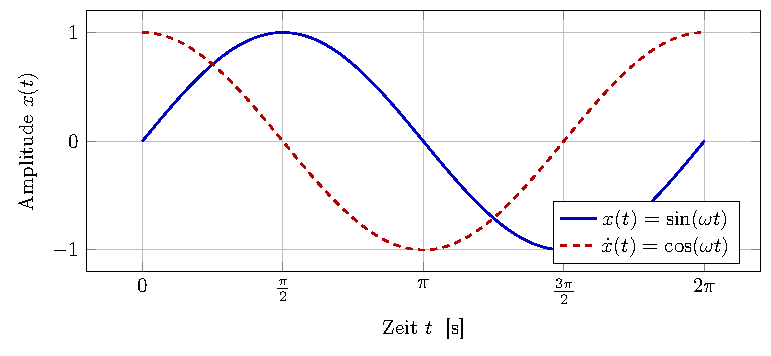
\includegraphics{fig01_sinus_ableitung}
	\caption{Kontinuierliches Sinussignal und seine Ableitung — mathematisch exakt, physikalisch unerreichbar.}
\end{figure}

\section{Energie und Bandbreite}

Die Energie eines kontinuierlichen Signals über einen endlichen Zeitraum:
\[
	E = \int_{-\infty}^{+\infty} |x(t)|^2 \, dt
\]
ist nur dann endlich, wenn $x(t) \in L^2(\mathbb{R})$. 
Jede reale Quelle kann nur eine \emph{endliche Gesamtenergie} liefern. 
Die dazu gehörende Fouriertransformierte:
\[
	X(f) = \mathcal{F}\{x(t)\} = \int_{-\infty}^{+\infty} x(t)\, e^{-j2\pi ft} \, dt
\]
hat für jedes physikalisch realisierbare Signal eine \textbf{endliche Bandbreite} $B$.
Damit kann kein reales System ein echtes Dirac-Impuls $\delta(t)$ erzeugen oder 
ein exaktes Kontinuum abbilden.

\section{Grenzen der Analog-Technik}

Die wichtigsten physikalischen Grenzen jedes realen Systems sind:

\begin{center}
\begin{tabular}{lll}
\toprule
\textbf{Eigenschaft} & \textbf{Ideal (Mathematik)} & \textbf{Real (Physik)} \\
\midrule
Zeitauflösung & $\Delta t \to 0$ & $\Delta t \geq \frac{1}{2B}$ \\
Amplitudenauflösung & $\Delta x \to 0$ & $\Delta x \geq \frac{u_{\max}}{2^N}$ \\
Speicherdauer & $\infty$ & endlich \\
Rauschen & keines & $U_N = \sqrt{4k_B T R \Delta f}$ \\
Energiebedarf & endlich & wächst mit Bandbreite \\
\bottomrule
\end{tabular}
\end{center}

Das thermische Rauschen einer realen Messschaltung beträgt:
\[
	U_N = \sqrt{4 k_B T R \Delta f}
\]
mit der Boltzmann-Konstante $k_B = \SI{1.38e-23}{\joule\per\kelvin}$, 
Temperatur $T$, Widerstand $R$ und Rauschbandbreite $\Delta f$.
Bereits dieses Rauschen setzt der Amplitudenauflösung eine absolute physikalische Grenze.

%=========================================================
\chapter{Das Abtasttheorem — Shannon und Nyquist}

\section{Die fundamentale Aussage}

Das Nyquist-Shannon-Abtasttheorem legt fest, unter welchen Bedingungen 
ein bandbegrenztes kontinuierliches Signal \emph{vollständig} durch 
diskrete Abtastwerte repräsentiert werden kann:

\begin{quote}
\itshape
Ein Signal $x(t)$ mit maximaler Frequenz $f_{\max}$ 
ist durch seine Abtastwerte vollständig beschrieben, 
wenn die Abtastfrequenz
\[
	f_s \geq 2 f_{\max} = f_N
\]
beträgt. Die Frequenz $f_N = 2f_{\max}$ heißt \textbf{Nyquistfrequenz}.
\end{quote}

Die vollständige Rekonstruktion ergibt sich durch Interpolation mit der sinc-Funktion:
\[
	x(t) = \sum_{n=-\infty}^{+\infty} x[n] \cdot \mathrm{sinc}\!\left(\frac{t - nT_s}{T_s}\right)
\]
mit $\mathrm{sinc}(u) = \frac{\sin(\pi u)}{\pi u}$ und $T_s = \frac{1}{f_s}$.

\section{Aliasing bei Unterabtastung}

Wird das Signal mit $f_s < 2f_{\max}$ abgetastet, entsteht \textbf{Aliasing}: 
Spektralanteile falten sich in den Basisband zurück und verfälschen das Signal irreversibel.
\[
	f_{\text{alias}} = \left| f_{\text{Signal}} - k \cdot f_s \right|, \quad k \in \mathbb{Z}
\]

\begin{figure}[H]
	\centering
	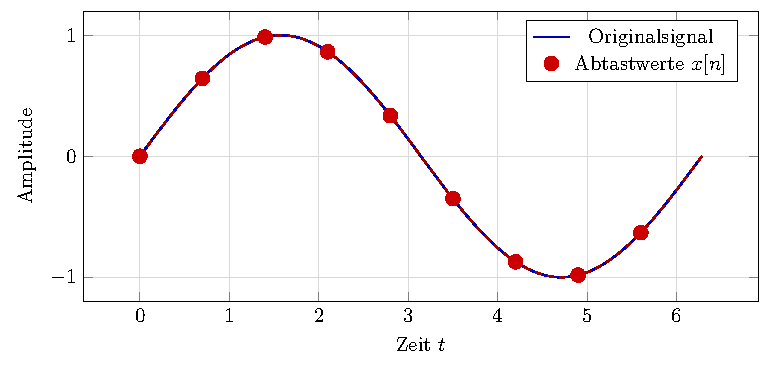
\includegraphics{fig02_abtastung}
	\caption{Abtastung eines Sinussignals: rote Punkte sind die diskreten Abtastwerte — 
	sie enthalten \emph{alle} physikalisch nutzbaren Informationen des Signals.}
\end{figure}

\section{Quantisierung}

Neben der Zeitdiskretisierung ist auch die \textbf{Amplitudenquantisierung} notwendig. 
Bei einem $N$-Bit-Wandler gelten:
\[
	\Delta u = \frac{u_{\max} - u_{\min}}{2^N}, \qquad
	\text{SNR}_{\text{max}} \approx 6{,}02\,N + 1{,}76 \; \text{dB}
\]

\begin{figure}[H]
	\centering
	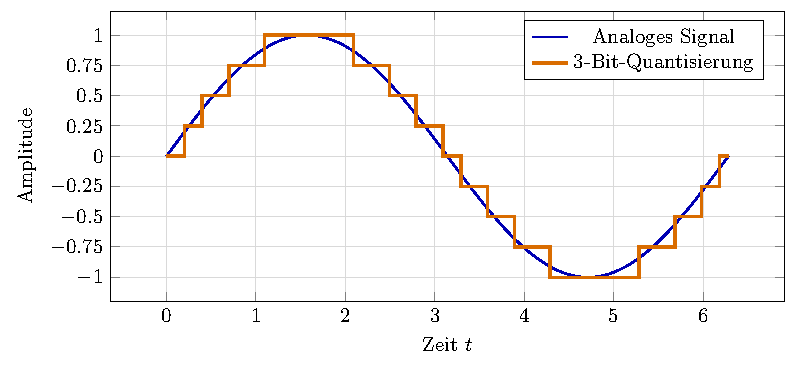
\includegraphics{fig03_quantisierung}
	\caption{Quantisierungsfehler bei 3-Bit-Auflösung: die Treppenstufen zeigen 
	die Abweichung vom Originalsignal.}
\end{figure}

%=========================================================
\chapter{Diskretisierung als Realitätsmodell}

\section{Physikalische Begründung}

Die diskrete Beschreibung durch:
\[
	x[n] = x(n T_s), \quad n \in \mathbb{Z}, \quad T_s = \frac{1}{f_s}
\]
ist kein Kompromiss — sie ist die \emph{physikalisch natürliche} Beschreibung.
Bereits die Quantenmechanik lehrt uns, dass Energie in diskreten Paketen 
(Quanten) übertragen wird:
\[
	E = h f = \hbar \omega, \quad h = \SI{6.626e-34}{\joule\second}
\]
Die Natur selbst ist diskret. Das Kontinuum ist die menschliche Abstraktion.

\section{Informationsgehalt}

Nach Shannon ist der maximale Informationsgehalt eines bandbegrenzten Kanals:
\[
	C = B \log_2\!\left(1 + \frac{S}{N}\right) \quad \left[\frac{\text{bit}}{\text{s}}\right]
\]
mit Bandbreite $B$, Signalleistung $S$ und Rauschleistung $N$.
Dieser Wert ist \emph{endlich} — ein Beweis dafür, dass keine unbegrenzte 
Informationsmenge übertragen werden kann.

\section{Vorteile der diskreten Beschreibung}

\begin{itemize}[leftmargin=2em]
	\item \textbf{Reproduzierbarkeit}: Digitale Daten können fehlerkorrigiert übertragen werden.
	\item \textbf{Speichereffizienz}: Kompression (MP3, JPEG, MPEG) setzt Diskretion voraus.
	\item \textbf{Verarbeitungsgeschwindigkeit}: DSP-Prozessoren erreichen $> \SI{10}{\giga\text{FLOPS}}$.
	\item \textbf{Präzision}: 24-Bit-Audio hat ein theoretisches SNR von $\approx \SI{144}{\decibel}$.
	\item \textbf{Universalität}: Jeder physikalische Prozess kann digital modelliert werden.
\end{itemize}

%=========================================================
\chapter{Vom akustischen Signal zur elektrischen Membran}

\section{Die akustische Druckwelle}

Schall ist eine mechanische Longitudinalwelle, beschrieben durch:
\[
	p(x,t) = p_0 \sin(\omega t - kx) + p_{\text{amb}}
\]
mit Schalldruckamplitude $p_0$, Wellenzahl $k = \omega/c$ 
und Schallgeschwindigkeit $c \approx \SI{343}{\meter\per\second}$ in Luft.

\begin{figure}[H]
	\centering
	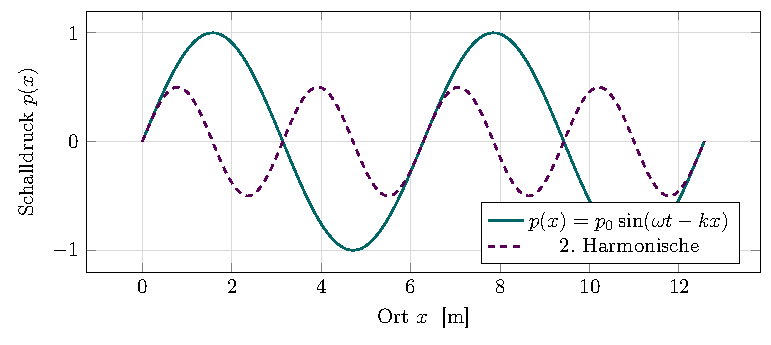
\includegraphics{fig04_druckwelle}
	\caption{Akustische Druckwelle und ihre zweite Harmonische.}
\end{figure}

Die Intensität der Schallwelle berechnet sich zu:
\[
	I = \frac{p_0^2}{2\rho c}
\]
mit Luftdichte $\rho \approx \SI{1.2}{\kilogram\per\cubic\meter}$.

\section{Schalldruckpegel und Wahrnehmung}

Der Schalldruck wird logarithmisch in Dezibel angegeben:
\[
	L_p = 20 \log_{10}\!\left(\frac{p}{p_0}\right) \; \text{dB}, 
	\quad p_0 = \SI{20}{\micro\pascal}
\]
Das menschliche Gehör verarbeitet Pegel von $0$ bis $\SI{130}{\decibel}$ — 
ein Dynamikbereich von über $10^6$. Diese enorme Spreizung ist nur durch 
nichtlineare, \emph{logarithmische Diskretisierung} im Innenohr möglich.

%=========================================================
\chapter{Die Membran als mechanisch-elektrisches System}

\section{Mechanisches Modell}

Eine ideale schwingende Membran wird durch die gedämpfte harmonische Schwingung beschrieben:
\[
	m\ddot{x}(t) + r\dot{x}(t) + k\,x(t) = F(t)
\]
mit Masse $m$ [\si{\kilogram}], Dämpfungskonstante $r$ [\si{\newton\second\per\meter}] 
und Federkonstante $k$ [\si{\newton\per\meter}].

Die Eigenfrequenz der ungedämpften Schwingung:
\[
	\omega_0 = \sqrt{\frac{k}{m}}, \qquad f_0 = \frac{\omega_0}{2\pi}
\]

\section{Mechanisches Ersatzschaltbild}

\begin{figure}[H]
	\centering
	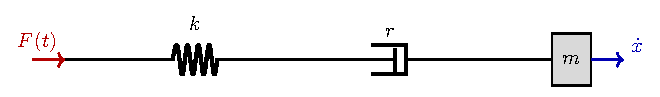
\includegraphics{fig05_membran_modell}
	\caption{Mechanisches Modell der Membran: Feder (Steifigkeit), Dämpfer (Verlust), Masse (Trägheit).}
\end{figure}

\section{Eigenfrequenz und Dämpfung}

Der Dämpfungsgrad $D$ bestimmt das Schwingungsverhalten:
\[
	D = \frac{r}{2\sqrt{mk}}
\]
\begin{itemize}[leftmargin=2em]
	\item $D < 1$: Untergedämpft — schwingende Bewegung, typisch für Membranen.
	\item $D = 1$: Kritische Dämpfung — schnellste Rückkehr ohne Überschwingen.
	\item $D > 1$: Übergedämpft — kriechende Rückkehr.
\end{itemize}

Die gedämpfte Eigenfrequenz:
\[
	\omega_d = \omega_0 \sqrt{1 - D^2}
\]

%=========================================================
\chapter{Elektrotechnisches Analogon der Membran}

\section{Mechanik–Elektrik-Analogie}

Die vollständige Analogie zwischen mechanischem und elektrischem System lautet:

\begin{center}
\begin{tabular}{lll}
\toprule
\textbf{Mechanisch} & \textbf{Symbol} & \textbf{Elektrisch} \\
\midrule
Kraft & $F$ & Spannung $U$ \\
Geschwindigkeit & $v = \dot{x}$ & Strom $I$ \\
Masse & $m$ & Induktivität $L$ \\
Federkonstante & $1/k$ & Kapazität $C$ \\
Dämpfung & $r$ & Widerstand $R$ \\
Verschiebung & $x$ & Ladung $q$ \\
\bottomrule
\end{tabular}
\end{center}

\section{RLC-Reihenschwingkreis}

\begin{figure}[H]
	\centering
	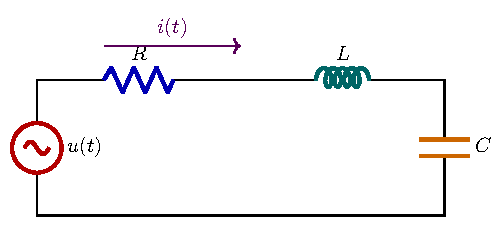
\includegraphics{fig06_rlc_schaltung}
	\caption{RLC-Reihenschwingkreis als elektrisches Analogon der schwingenden Membran.}
\end{figure}

Die Maschengleichung des RLC-Kreises:
\[
	L\ddot{q}(t) + R\dot{q}(t) + \frac{1}{C}q(t) = u(t)
\]
Mit $i(t) = \dot{q}(t)$ folgt die Differentialgleichung für den Strom:
\[
	L\dot{i}(t) + R\,i(t) + \frac{1}{C}\int i(\tau)\,d\tau = u(t)
\]

\section{Eigenfrequenz und Güte}

Die Resonanzfrequenz des RLC-Kreises:
\[
	\omega_0 = \frac{1}{\sqrt{LC}}, \qquad f_0 = \frac{1}{2\pi\sqrt{LC}}
\]
Die Güte (Qualitätsfaktor) beschreibt die Selektivität:
\[
	Q = \frac{1}{R}\sqrt{\frac{L}{C}} = \frac{\omega_0 L}{R} = \frac{1}{\omega_0 C R}
\]
Ein hoher $Q$-Wert entspricht einer scharfen Frequenzselektivität — 
genau wie ein bestimmter Abschnitt der Basilarmembran selektiv auf eine 
schmale Frequenzband reagiert.

\section{Impedanz und Frequenzgang}

Die komplexe Impedanz des RLC-Kreises:
\[
	\underline{Z}(\omega) = R + j\omega L + \frac{1}{j\omega C} 
		= R + j\!\left(\omega L - \frac{1}{\omega C}\right)
\]
Der Betrag des Frequenzgangs:
\[
	|\underline{Z}(\omega)| = \sqrt{R^2 + \left(\omega L - \frac{1}{\omega C}\right)^2}
\]
Bei Resonanz ($\omega = \omega_0$) gilt $\underline{Z}(\omega_0) = R$ — minimale Impedanz, maximaler Strom.

\begin{figure}[H]
	\centering
	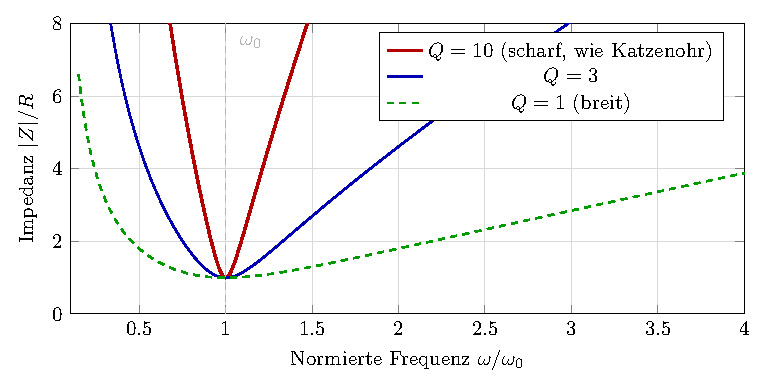
\includegraphics{fig07_impedanz_rlc}
	\caption{Impedanzverlauf des RLC-Kreises für verschiedene Gütefaktoren: 
	hohe Güte entspricht enger Frequenzselektivität — das Prinzip der Basilarmembran.}
\end{figure}

\section{Phasenverhalten von Spule und Kondensator — die Merkregel}

\subsection*{Fundamentales Kausalitätsprinzip: Der Strom eilt physikalisch immer nach.}

Dies ist keine bloße Merkregel, sondern ein tief verwurzeltes physikalisches Prinzip:
\emph{In jedem realen Stromkreis ist die Spannung die Ursache, der Strom die Wirkung.}
Keine Wirkung kann ihrer Ursache vorauseilen.
Daher gilt ohne Ausnahme:

\begin{quote}
\itshape
Der Strom ist stets die kausale Antwort auf die anliegende Spannung —
er eilt physikalisch immer nach.
Für die Spule ist dies unmittelbar anschaulich (Lenz'sches Gesetz);
für den Kondensator ergibt es sich aus dem Prinzip, dass die angelegte Spannung
(Ursache) die Ladungsverschiebung (Strom als Wirkung) erzeugt.
Die Impedanzrichtung im Zeigerdiagramm — \textbf{links herum} bei der Spule,
\textbf{rechts herum} beim Kondensator — beschreibt lediglich die
\emph{geometrische Orientierung} dieses Nacheilens in der komplexen Ebene.
\end{quote}

\begin{center}
\renewcommand{\arraystretch}{1.4}
\begin{tabular}{p{7.5cm} p{7.5cm}}
\toprule
\textbf{1.1 — Spule (Induktivität): links herum, Strom eilt nach}
& \textbf{1.2 — Kondensator (Kapazität): rechts herum, Strom eilt nach} \\
\midrule
Impedanz $\underline{Z}_L = j\omega L$ zeigt in die \emph{positive} imaginäre
Richtung — \textbf{links herum} (entgegen dem Uhrzeigersinn) in der
komplexen Ebene. Der Strom eilt der Spannung um $90°$ \emph{nach}.
& Impedanz $\underline{Z}_C = -\tfrac{j}{\omega C}$ zeigt in die
\emph{negative} imaginäre Richtung — \textbf{rechts herum} (im Uhrzeigersinn)
in der komplexen Ebene. Der Strom eilt nach:
die angelegte Spannung verursacht die Ladungsverschiebung, nicht umgekehrt. \\
\bottomrule
\end{tabular}
\end{center}

\paragraph{1.1 \quad Spule — Impedanz links herum, Strom eilt nach.}

Im Zeitbereich gilt für eine ideale Induktivität die fundamentale Beziehung:
\[
	u_L(t) = L\,\frac{d\,i_L(t)}{dt}
\]
Mit dem Ansatz $i_L(t) = I_0\cos(\omega t)$ als Referenzgröße ergibt sich:
\[
	u_L(t) = -L\,\omega\,I_0 \sin(\omega t) = L\,\omega\,I_0\,\cos\!\left(\omega t + \frac{\pi}{2}\right)
\]
Die Spannung $u_L(t)$ erreicht ihr Maximum um eine Viertelperiode $T/4$ \emph{früher}
als der Strom — der Strom kommt \emph{nach}. In der komplexen Zeigerschreibweise:
\[
	\underline{U}_L = j\omega L \cdot \underline{I} = \omega L \cdot e^{+j\pi/2} \cdot \underline{I}
\]
Der Multiplikationsfaktor $e^{+j\pi/2} = j$ dreht den Spannungszeiger um $+90°$
\emph{entgegen dem Uhrzeigersinn} — das ist die Richtung \textbf{links herum} in der
Gaußschen Zahlenebene. Der Impedanzzeiger $\underline{Z}_L = j\omega L$ liegt daher auf der
\emph{positiven imaginären Halbachse}.

\begin{align}
	&\varphi_{U_L} - \varphi_{I_L} = +90° \\[4pt]
	&\Longrightarrow \quad
	\text{Strom eilt der Spannung um } 90° \text{ nach}
	\quad (\varphi_{I} = \varphi_{U} - 90°)
\end{align}

Physikalische Begründung: Die Induktivität \emph{widersetzt sich} Stromänderungen durch
ihre Gegen-EMK (Lenz'sches Gesetz). Eine angelegte Spannungsänderung erzeugt erst mit
zeitlicher Verzögerung einen Anstieg des Stroms — der Strom \emph{hinkt} der Spannung
nach. Das Kausalitätsprinzip ist hier am direktesten sichtbar:
Spannung anlegen $\to$ Gegenkraft aufgebaut $\to$ Strom steigt langsam an.

\paragraph{1.2 \quad Kondensator — Impedanz rechts herum, Strom eilt nach.}

Am Kondensator gilt:
\[
	i_C(t) = C\,\frac{d\,u_C(t)}{dt}
\]
Die Ladungsverschiebung (Strom) ist proportional zur \emph{Änderungsrate} der
anliegenden Spannung — sie ist die direkte kausale Antwort auf die Spannungsänderung.
Kein Strom fließt ohne eine treibende Spannung.

Die Impedanz des Kondensators:
\[
	\underline{Z}_C = \frac{\underline{U}_C}{\underline{I}_C} = \frac{1}{j\omega C} = -\frac{j}{\omega C}
	= \frac{1}{\omega C}\cdot e^{-j\pi/2}
\]
Der Faktor $e^{-j\pi/2} = -j$ dreht den Impedanzzeiger um $-90°$ — das entspricht der
Richtung \textbf{rechts herum} (im Uhrzeigersinn) in der komplexen Ebene.

\begin{align}
	&\varphi_{U_C} - \varphi_{I_C} = -90° \\[4pt]
	&\Longrightarrow \quad
	\text{Strom eilt nach (Kausalität):}
	\quad \text{anliegende Spannung} \;\\
	& \Longrightarrow \quad \text{Ladungsverschiebung als Wirkung}
\end{align}

Physikalische Begründung durch das Kausalitätsprinzip:
Die anliegende Spannung (Ursache) erzeugt das elektrische Feld im Dielektrikum und
treibt damit die Ladungsträger an die Kondensatorplatten — dies ist der Strom (Wirkung).
Kein Strom kann fließen, ohne dass zuvor eine Potentialdifferenz angelegt wurde.
Der Strom ist daher die kausale Folge der Spannung: er eilt nach.

Die Kondensatorspannung $u_C(t)$ ihrerseits ist die zeitliche Aufsummierung (Integration)
des geflossenen Stroms:
\[
	u_C(t) = \frac{1}{C}\int_0^t i_C(\tau)\,d\tau + u_C(0)
\]
Dies bedeutet: die \textbf{Kondensatorspannung} ist die \emph{Wirkung des Stroms} und
eilt dem Strom nach — nicht umgekehrt. Die Impedanzrichtung \textbf{rechts herum} ($-j$)
ist das formale Abbild dieser kausalen Orientierung in der komplexen Ebene.

\begin{figure}[H]
	\centering
	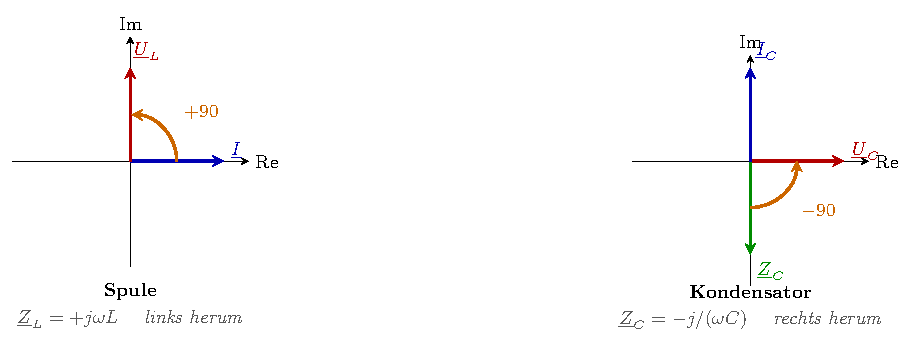
\includegraphics{fig08_zeigerdiagramme}
	\caption{Zeigerdiagramme in der komplexen Impedanzebene.
	\textbf{Links}: Spule — Impedanzzeiger \emph{links herum} ($+j$): die Spannung
	$\underline{U}_L$ eilt vor, der \textcolor{blue!70!black}{Strom $\underline{I}$} (blau)
	eilt \textbf{nach} (Lenz'sches Gesetz).
	\textbf{Rechts}: Kondensator — Impedanzzeiger \emph{rechts herum} ($-j$):
	die Spannung $\underline{U}_C$ (rot) ist die kausale Ursache;
	der \textcolor{blue!70!black}{Strom $\underline{I}_C$} ist die Wirkung —
	er eilt \textbf{nach} (Kausalitätsprinzip: Spannung $\to$ Ladungsverschiebung).}
\end{figure}

\begin{figure}[H]
	\centering
	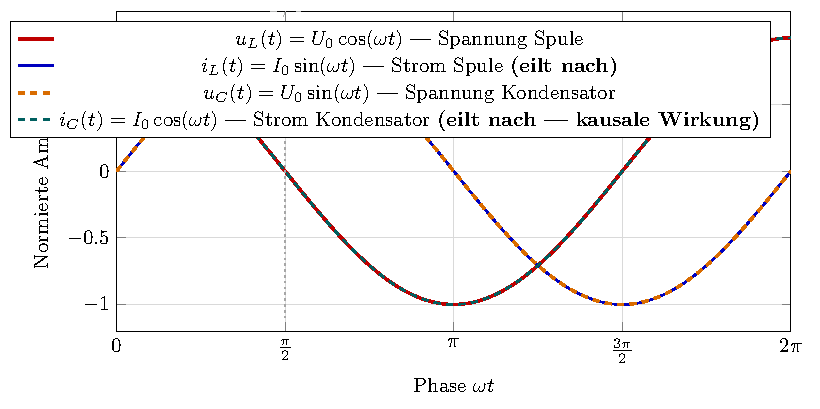
\includegraphics{fig09_phasenvergleich}
	\caption{Phasenvergleich im Zeitbereich — in beiden Fällen eilt der Strom nach.
	\textbf{Spule} (durchgezogen): Der \textcolor{blue!75!black}{Strom $i_L(t)$} (blau)
	folgt der \textcolor{red!75!black}{Spannung $u_L(t)$} (rot) mit $T/4$ — Strom \emph{eilt nach}.
	\textbf{Kondensator} (gestrichelt): Die \textcolor{orange!85!black}{Kondensatorspannung $u_C(t)$}
	(orange) ist die zeitliche Integration des \textcolor{teal!75!black}{Stroms $i_C(t)$} (türkis) —
	die Spannung \emph{eilt dem Strom nach}; der Strom ist die kausale Antwort auf die
	angelegte treibende Spannung (Ursache $\to$ Wirkung). Impedanzrichtung: \emph{rechts herum}.}
\end{figure}

\paragraph{Bedeutung für das RLC-Membranmodell.}
Im RLC-Schwingkreis als elektrotechnisches Analogon der schwingenden Membran
überlagern sich Spulen- und Kondensatorverhalten frequenzabhängig:
\begin{itemize}[leftmargin=2em]
	\item Bei $\omega < \omega_0$: \textbf{kapazitiv dominiert} —
		Impedanz \emph{rechts herum} ($-j$).
		Der Strom eilt nach (Kausalität: Kondensator-Spannung ist Wirkung des Stroms,
		der sich seinerseits auf die angelegte Quelle als Ursache antwortend aufbaut).
		Die Membran verhält sich wie eine \emph{nachgebende} Feder.
	\item Bei $\omega = \omega_0$: \textbf{Resonanz} —
		induktiver und kapazitiver Anteil kompensieren einander exakt ($\underline{Z} = R$,
		rein reell), maximaler Strom in Phase mit der Spannung (minimales Nacheilen).
		Dies entspricht dem mechanischen Resonanzpunkt der Membran.
	\item Bei $\omega > \omega_0$: \textbf{induktiv dominiert} —
		Impedanz \emph{links herum} ($+j$).
		Der Strom eilt nach (Lenz'sches Gesetz: Magnetfeld wirkt der Stromänderung entgegen).
		Die Membran verhält sich wie eine träge Masse.
\end{itemize}

\textbf{Fazit:} In beiden Frequenzbereichen und an beiden reaktiven Bauelementen gilt
das gleiche fundamentale Kausalitätsprinzip: der Strom ist die physikalische Antwort
auf die antreibende Spannung und eilt ihr nach — nur die \emph{geometrische Richtung}
dieses Nacheilens im Zeigerdiagramm ist verschieden:
Links herum (Spule, $\omega > \omega_0$) oder rechts herum (Kondensator, $\omega < \omega_0$).
Diese Phasenumkehr an der Resonanzfrequenz $\omega_0$ ist das elektrotechnische Abbild
jenes Moments, in dem die Membran von Federdominanz zu Massenträgheitsdominanz
wechselt — das fundamentale Spektralanalyseprinzip der Basilarmembran.

%=========================================================
\chapter{Spannungs- und Stromverläufe im RLC-System}

\section{Freie gedämpfte Schwingung}

Bei einem Energiestoß $u_0$ zur Zeit $t=0$ schwingt der RLC-Kreis frei aus.
Die Lösung der homogenen Differentialgleichung für den Unterdämpfungsfall:
\[
	u_C(t) = U_0 \left(1 - e^{-\alpha t}\cos(\omega_d t + \varphi)\right), 
	\quad \alpha = \frac{R}{2L}, \quad \omega_d = \sqrt{\omega_0^2 - \alpha^2}
\]

\begin{figure}[H]
	\centering
	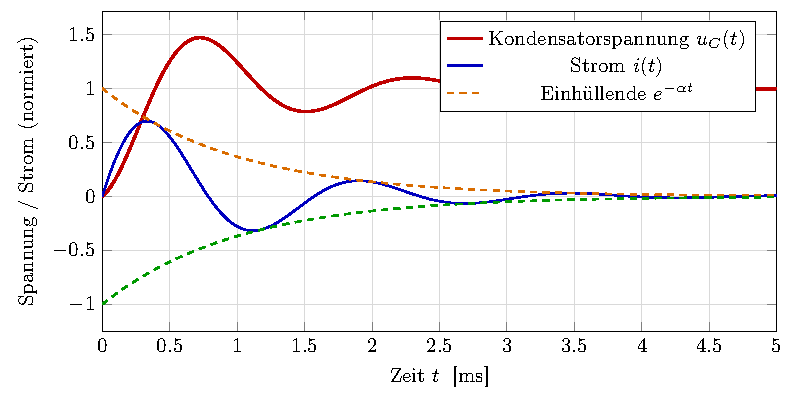
\includegraphics{fig10_sprungantwort}
	\caption{RLC-Sprungantwort: \textcolor{red!70!black}{Kondensatorspannung $u_C(t)$} 
	(rot), \textcolor{blue!70!black}{Strom $i(t)$} (blau) und 
	\textcolor{orange!80!black}{Einhüllende} (orange gestrichelt). 
	Klassisches Verhalten einer schwingenden Membran.}
\end{figure}

\section{Einzelkomponenten-Spannungen}

\begin{figure}[H]
	\centering
	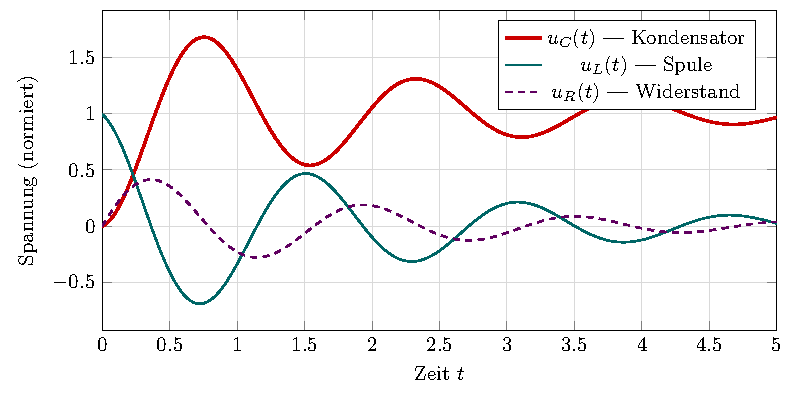
\includegraphics{fig11_spannungsaufteilung}
	\caption{Spannungsaufteilung im RLC-Kreis: Kondensator (rot), Spule (türkis), 
	Widerstand (violett). Die Summe ergibt zu jederzeit die Quellenspannung.}
\end{figure}

\section{Erzwungene Schwingung — Resonanzverhalten}

Bei sinusförmiger Erregung mit variabler Frequenz zeigt der RLC-Kreis Resonanzverhalten:

\begin{figure}[H]
	\centering
	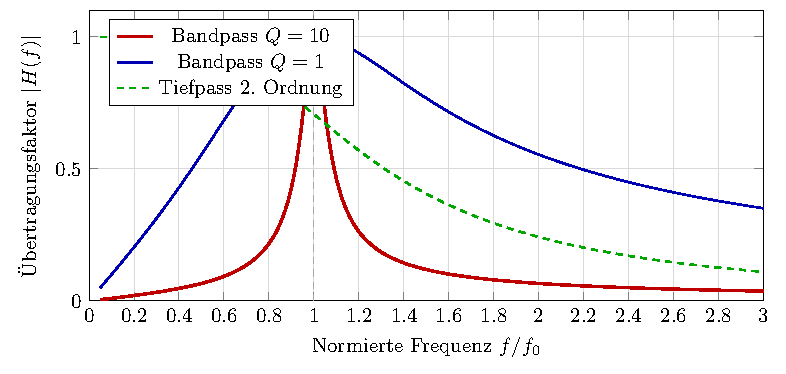
\includegraphics{fig12_frequenzgaenge}
	\caption{Frequenzgänge: Bandpass mit hoher Güte $Q=10$ (rot) 
	— das elektrische Modell eines Basilarmembran-Segments.}
\end{figure}

%=========================================================
\chapter{Die Membran als biologischer Diskretisierer}

\section{Aufbau und Funktion}

Die biologische Membran besitzt eine einzigartige Kombination von Eigenschaften, 
die sie zum idealen Diskretisierungsmechanismus machen:

\begin{itemize}[leftmargin=2em]
	\item \textbf{Schwellenwert (Threshold)}: Ein Signal wird erst dann weitergeleitet, 
		wenn eine bestimmte Reizschwelle überschritten wird.
	\item \textbf{Aktionspotential}: Nach dem Alles-oder-Nichts-Prinzip: entweder voller Impuls 
		oder keiner — binäre Diskretisierung.
	\item \textbf{Refraktärzeit}: Die Membran ist nach einem Impuls kurzzeitig 
		inexzitabel — das entspricht der minimalen Abtastperiode $T_s = 1/f_s$.
	\item \textbf{Frequenzcodierung}: Die Rate der Aktionspotentiale codiert die Intensität — 
		Pulsweitenmodulation (PWM) in der Natur.
\end{itemize}

\section{Hodgkin-Huxley-Modell (vereinfacht)}

Das vereinfachte elektrische Modell der Nervenmembran:
\[
	C_m \frac{du_m}{dt} = -g_{Na}(u_m - E_{Na}) - g_K(u_m - E_K) - g_L(u_m - E_L) + I_{\text{ext}}
\]
mit Membrankapazität $C_m$, Leitfähigkeiten $g_{Na}$, $g_K$, $g_L$ und 
Umkehrpotentialen $E_{Na}$, $E_K$, $E_L$.

\begin{figure}[H]
	\centering
	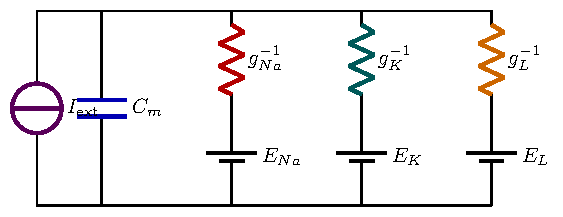
\includegraphics{fig13_hodgkin_huxley}
	\caption{Elektrisches Ersatzschaltbild der Nervenmembran nach Hodgkin-Huxley: 
	Membrankapazität und ionische Leitfähigkeitskanäle.}
\end{figure}

\section{Das Aktionspotential — diskretes Muster}

\begin{figure}[H]
	\centering
	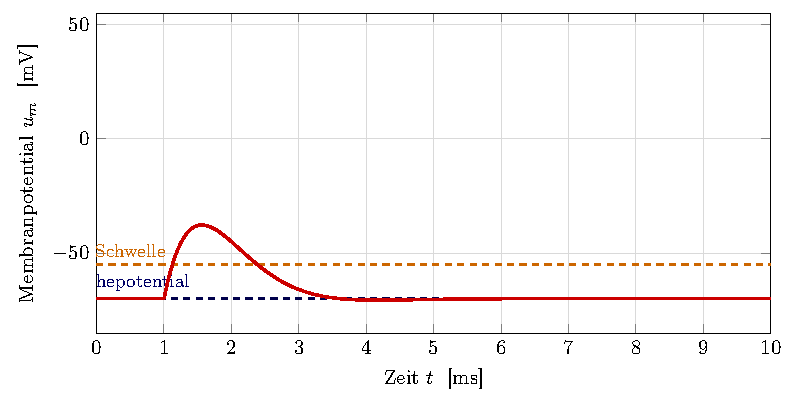
\includegraphics{fig14_aktionspotential}
	\caption{Schematisches Aktionspotential einer Nervenzelle: 
	Ruhepotential (blau), Schwellenpotential (orange), 
	Aktionspotential (rot) — das fundamentale diskrete Ereignis der Natur.}
\end{figure}

\section{Schwellwert-Schaltung als technisches Analogon}

\begin{figure}[H]
	\centering
	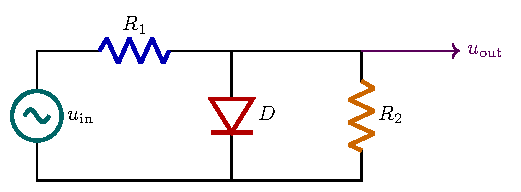
\includegraphics{fig15_schwellwert}
	\caption{Schwellwertschaltung mit Diode: 
	erst wenn $u_{\text{in}} > U_{\text{th}}$ gibt die Schaltung ein Signal weiter — 
	das technische Pendant zum biologischen Aktionspotential.}
\end{figure}

%=========================================================
\chapter{Das Digitalsignal — Geburt der Information}

\section{Vom analogen Signal zum Bitstrom}

Der vollständige A/D-Wandlungsprozeß umfasst:
\begin{enumerate}[leftmargin=2em]
	\item \textbf{Tiefpassfilterung} (Anti-Aliasing-Filter) auf $f < f_s/2$,
	\item \textbf{Abtastung} mit $f_s \geq 2 f_{\max}$,
	\item \textbf{Quantisierung} auf $2^N$ Stufen,
	\item \textbf{Codierung} als Binärwort der Breite $N$ Bit.
\end{enumerate}

\begin{figure}[H]
	\centering
	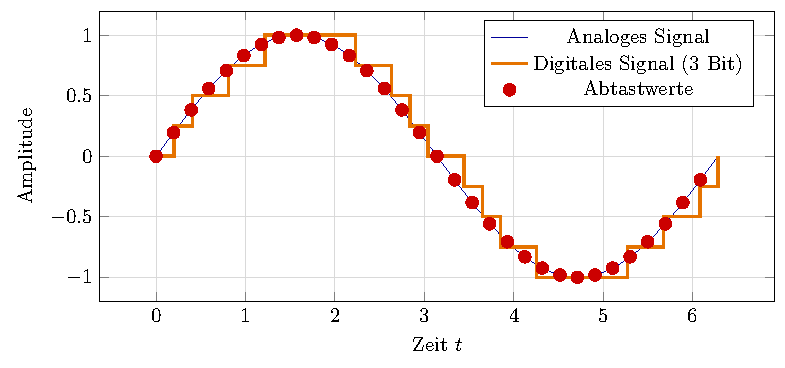
\includegraphics{fig16_ad_wandlung}
	\caption{A/D-Wandlung: analoges Signal (blau, dünn), 
	quantisiertes Digitalsignal (orange, treppenförmig) 
	und diskrete Abtastwerte (rote Punkte).}
\end{figure}

\section{Binäres Pulssignal — Informationsträger}

\begin{figure}[H]
	\centering
	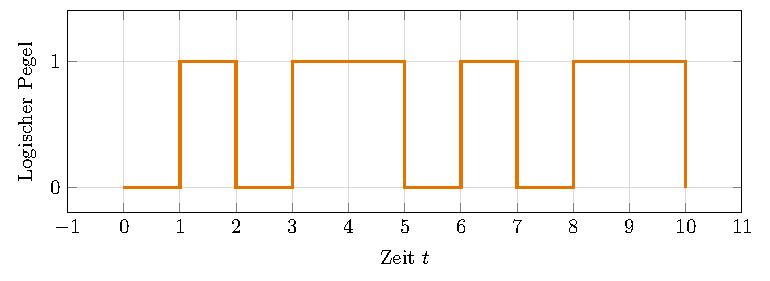
\includegraphics{fig17_bitfolge}
	\caption{Bitfolge nach Digitalisierung: Jeder Pegel ist ein diskretes Ereignis — 
	hier entsteht Information im Sinne Shannons.}
\end{figure}

%=========================================================
\chapter{Das Gehör der Katze — optimale biologische Membran}

\section{Warum die Katze?}

Das Gehör der Katze gilt als das ausgereifteste Säugetier-Gehörsystem 
und ist das beste biologische Vorbild für eine optimale Membran:

\begin{itemize}[leftmargin=2em]
	\item \textbf{Frequenzbereich}: \SIrange{48}{85000}{\hertz} — 
		weit über dem menschlichen Bereich von \SIrange{20}{20000}{\hertz}.
	\item \textbf{Richtungshören}: Wendbares Außenohr (Pinna) mit $\pm 180°$ — 
		aktive mechanische Vorverarbeitung.
	\item \textbf{Dynamikbereich}: $> \SI{100}{\decibel}$ durch logarithmische Energie-Codierung.
	\item \textbf{Zeitauflösung}: $< \SI{100}{\micro\second}$ — 
		höher als bei jedem technischen Mikrofon vergleichbarer Größe.
	\item \textbf{Aktive Verstärkung}: Äußere Haarzellen der Basilarmembran 
		agieren als aktive Verstärker mit neuronalem Feedback.
\end{itemize}

\section{Die Basilarmembran als Frequenzanalysator}

Die Basilarmembran der Katze kann als ortsverteilte Filterbank modelliert werden:
\[
	f_0(x) = f_{\text{apex}} \cdot e^{\,\beta x}, \quad 0 \leq x \leq L
\]
mit Ortsvariable $x$, Resonanzfrequenz am Apex $f_{\text{apex}} \approx \SI{200}{\hertz}$ 
und Skalierungsparameter $\beta$.

\begin{figure}[H]
	\centering
	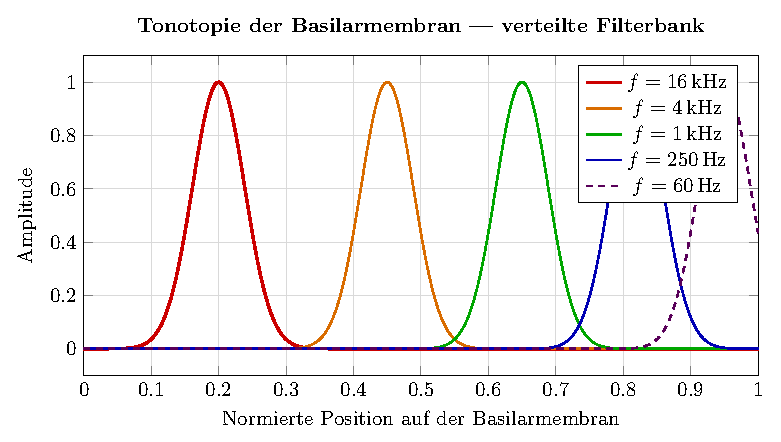
\includegraphics{fig18_tonotopie}
	\caption{Tonotopie der Basilarmembran: jede Frequenz stimuliert einen 
	anderen Ort — Hochfrequenzen am Eingang (Basis), Tieffrequenzen an der Spitze (Apex).
	Das ist ein hochgradig selektives, räumlich verteiltes Spektralanalysatorsystem.}
\end{figure}

\section{Filterbank-Modell eines Basilarmembran-Segments}

Jedes Membransegment wirkt als schmalbandiger Bandpassfilter. 
Das elektrische Modell eines Segmentes:

\begin{figure}[H]
	\centering
	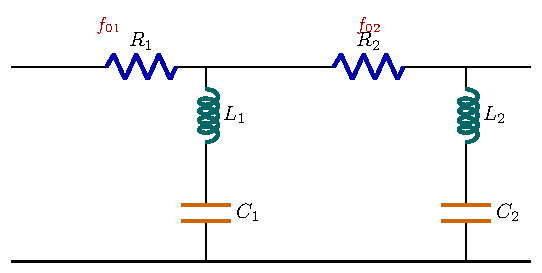
\includegraphics{fig19_filterbank}
	\caption{Mehrstufiges Filterbank-Modell der Basilarmembran: 
	jedes LC-Glied ist auf eine andere Frequenz $f_{0i}$ abgestimmt.}
\end{figure}

\section{Aktive Verstärkung — das Cochlear Amplifier-Prinzip}

Die äußeren Haarzellen erzeugen durch elektromotorische Kräfte 
(Prestin-Motorprotein) eine aktive mechanische Rückkopplung:
\[
	F_{\text{akt}}(t) = g_{\text{motor}} \cdot u_m(t)
\]
Dies entspricht einem negativen Widerstand im elektrischen Modell:
\[
	R_{\text{eff}} = R_{\text{passiv}} - g_{\text{motor}}
\]
Wenn $g_{\text{motor}} > R_{\text{passiv}}$, wird das System instabil — 
das Ohr kann selbst schwingen (\textit{otoakustische Emissionen}).

%=========================================================
\chapter{Vergleich der Katzenmembran mit der Hundmembran}

\section{Motivation und biologischer Rahmen}

Der Vergleich zweier nahe verwandter Säugetierspezies — Hauskatze (\textit{Felis catus})
und Haushund (\textit{Canis lupus familiaris}) — ist aus mehreren Gründen aufschlussreich.
Beide sind Beutegreifer bzw.~Raubtiere, beide haben sich evolutionär auf
akustische Signalverarbeitung spezialisiert, und dennoch zeigen ihre Hörsysteme
signifikante Unterschiede, die sich quantitativ analysieren und auf biophysikalische
Prinzipien zurückführen lassen.
Der Vergleich bietet damit einen kontrollierten Rahmen, um zu verstehen,
\emph{warum} gerade die Katzenmembran das physiologisch und informationstheoretisch
optimale Konstrukt darstellt.

\section{2.1 — Systematischer Vergleich: Katzenmembran vs.~Hundmembran}

\subsection{Messbare Parameter im direkten Vergleich}

\begin{center}
\renewcommand{\arraystretch}{1.45}
\begin{tabular}{p{5.0cm} p{4.5cm} p{4.5cm}}
\toprule
\textbf{Parameter} & \textbf{Katze} & \textbf{Hund} \\
\midrule
Frequenzbereich (Hörfeld)
  & \SIrange{48}{85000}{\hertz}
  & \SIrange{40}{65000}{\hertz} \\
Obergrenzfrequenz $f_{\max}$
  & $\approx\SI{85}{\kilo\hertz}$
  & $\approx\SI{65}{\kilo\hertz}$ \\
Nutzbare Bandbreite $B$
  & $\approx\SI{85}{\kilo\hertz}$
  & $\approx\SI{65}{\kilo\hertz}$ \\
Länge der Basilarmembran
  & $\approx\SI{25}{\milli\meter}$
  & $\approx\SI{32}{\milli\meter}$ \\
Tonotopischer Gradient $\beta$
  & $\approx\SI{2.1}{\milli\meter^{-1}}$
  & $\approx\SI{1.7}{\milli\meter^{-1}}$ \\
Mittlerer Gütefaktor $Q_{10\text{dB}}$
  & $Q \approx 8{,}5 \ldots 30$
  & $Q \approx 4 \ldots 12$ \\
Zeitauflösung (Jitter)
  & $< \SI{100}{\micro\second}$
  & $\approx \SI{300}{\ldots}\SI{500}{\micro\second}$ \\
Dynamikbereich
  & $>\SI{100}{\decibel}$
  & $\approx\SI{80}{\decibel}$ \\
Anzahl äußere Haarzellen
  & $\approx 10\,000$
  & $\approx 10\,500$ \\
Spiralganglionfasern (AN)
  & $\approx 50\,000$
  & $\approx 30\,000$ \\
Pinnabeweglichkeit
  & $\pm\,180°$, 32 Muskeln
  & $\pm\,90°$, ca.~18 Muskeln \\
Aktive Verstärkung (Prestin)
  & stark ausgeprägt
  & schwächer ausgeprägt \\
\bottomrule
\end{tabular}
\end{center}

\subsection{Frequenzgang und Bandbreite}

Der für die Diskretisierung und Informationsverarbeitung entscheidende Parameter ist
die \emph{nutzbare Bandbreite} $B$ des Hörsystems.
Nach Shannon gilt für die maximale Kanalkapazität:
\[
C = B\log_2\!\left(1 + \frac{S}{N}\right)
\]
Die Katze besitzt mit $B \approx \SI{85}{\kilo\hertz}$ eine um den Faktor
\[
\frac{B_{\text{Katze}}}{B_{\text{Hund}}} = \frac{85}{65} \approx 1{,}31
\]
größere Bandbreite als der Hund. Bei gleichem SNR ergibt sich damit eine um $31\,\%$
höhere maximale Informationskapazität.

Die Katze erreicht diese Bandbreite mit einer \emph{kürzeren Membran}
von $\approx\SI{25}{\milli\meter}$ gegenüber $\approx\SI{32}{\milli\meter}$ beim Hund.
Dies impliziert einen steileren tonotopischen Gradienten:
\[
\beta_{\text{Katze}} \approx \SI{2{,}1}{\milli\meter^{-1}}
\;>\;
\beta_{\text{Hund}} \approx \SI{1{,}7}{\milli\meter^{-1}}
\]
Der Parameter $\beta$ in der tonotopischen Abbildungsformel
$f_0(x) = f_{\text{apex}}\cdot e^{\beta x}$
bestimmt, wie viele Frequenzkanäle pro Millimeter Membranstrecke verfügbar sind.
Eine höhere Steilheit bedeutet \emph{mehr Frequenzselektivität pro Einheitslänge}.

\subsection{Gütefaktor und Frequenzselektivität}

Der $Q_{10\text{dB}}$-Wert ist ein Maß für die Schärfe der Abstimmung eines
einzelnen Basilarmembran-Segments. Er ist definiert als Verhältnis von
Eigenfrequenz zu Bandbreite $10\,\text{dB}$ unterhalb des Maximums:
\[
Q_{10\text{dB}} = \frac{f_0}{\Delta f_{10\text{dB}}}
\]

\begin{figure}[H]
	\centering
	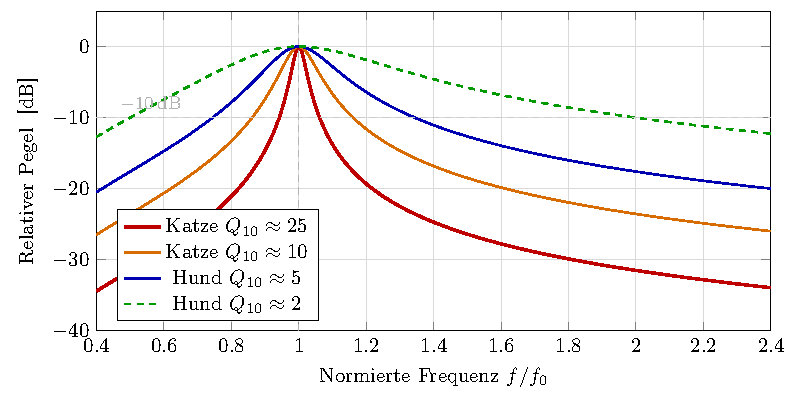
\includegraphics{fig20_guete_vergleich}
	\caption{Frequenzselektivität eines Basilarmembran-Segments im Vergleich.
\textcolor{red!75!black}{Rot}/\textcolor{orange!85!black}{orange}:
Bandpasscharakteristik typischer Katzenfasern ($Q_{10}\approx 10\ldots25$).
\textcolor{blue!70!black}{Blau}/\textcolor{green!60!black}{grün}: repräsentative
Hundfasern ($Q_{10}\approx 2\ldots5$).
Der $-10\,\text{dB}$-Pegel (gestrichelte Horizontale) definiert die $Q_{10}$-Bandbreite.}
\end{figure}

Der doppelt so hohe $Q$-Wert der Katze bedeutet direkt:
\[
\Delta f_{\text{Katze}} = \frac{f_0}{Q_{\text{Katze}}} \approx \frac{f_0}{20},
\qquad
\Delta f_{\text{Hund}} = \frac{f_0}{Q_{\text{Hund}}} \approx \frac{f_0}{7}
\]
Die \textbf{Frequenzauflösung} der Katzenmembran ist damit um den Faktor
$\approx 3$ feiner als beim Hund — bei gleicher Eigenfrequenz $f_0$.

\subsection{Zeitauflösung und neuronales Encoding}

Eine weitere kritische Größe ist die Zeitauflösung des Hörnervs,
gemessen als \emph{Jitter} des ersten Aktionspotentials nach einem
kurzen Schallimpuls:
\[
\sigma_{\text{Katze}} < \SI{100}{\micro\second},
\qquad
\sigma_{\text{Hund}} \approx \SI{300}{\ldots}\SI{500}{\micro\second}
\]
Diese Zeitauflösung bestimmt, mit welcher Präzision Laufzeitdifferenzen
zwischen den Ohren (Interaural Time Difference, ITD) ausgewertet werden können.
Das Katzengehirn kann Richtungsinformationen mit einer Winkelauflösung von
$\approx 1°$ berechnen, während der Hund nur auf $\approx 5{-}8°$ kommt.

Als äquivalente Nyquistfrequenz des Zeitkanals ausgedrückt:
\[
f_{s,\text{Zeit}} = \frac{1}{2\sigma}
\quad\Rightarrow\quad
\left.f_{s,\text{Zeit}}\right|_{\text{Katze}} = \SI{5}{\kilo\hertz},
\quad
\left.f_{s,\text{Zeit}}\right|_{\text{Hund}} \approx \SI{1}{\kilo\hertz}
\]
Die Katze besitzt demnach einen fünfmal feineren Zeitkanal für die Richtungslokalisation.

\subsection{Pinnageometrie als mechanische Vorverarbeitung}

Das bewegliche Außenohr (Pinna) beider Tiere wirkt als räumlicher Vorfilter:
\begin{itemize}[leftmargin=2em]
\item Die \textbf{Katze} kann jede Ohrmuschel unabhängig voneinander über
$\pm 180°$ rotieren. Mit 32 spezialisierten Ohrmuschelmuskeln ermöglicht
sie eine \emph{aktive akustische Abtastung} des Raumes ohne Kopfdrehung.
\item Der \textbf{Hund} besitzt etwa 18 Muskeln mit einem eingeschränkten
Bewegungsbereich von $\pm 90°$; Rasseunterschiede (Schlappohren vs.~Stehohren)
führen bei vielen Hunderassen zu einer deutlich reduzierten Richtwirkung.
\end{itemize}
In der Elektrotechnik entspricht dies einer aktiven Strahlformung (Beamforming):
die Katze realisiert ein richtungsanpassbares Mikrofon erster Ordnung,
der Hund im Mittel nur eine Kugelcharakteristik.

\section{2.2 — Beweis der Optimalität der Katzenmembran}
\label{sec:aktiv}

\subsection{Formulierung des Optimalitätskriteriums}

Damit ein biologisches Diskretisierungssystem als \emph{optimal} bezeichnet werden kann,
muss es unter den gegebenen physikalischen Randbedingungen
(endliche Cochlea-Länge $L$, endliche Energieversorgung, finites SNR des Mediums Luft)
die \emph{maximale Shannonsche Kanalkapazität}
\[
C = \int_0^{f_{\max}} \log_2\!\left(1 + \frac{S(f)}{N(f)}\right)df \quad \left[\frac{\mathrm{bit}}{\mathrm{s}}\right]
\]
realisieren. Die Optimierung muss dabei drei Teilziele gleichzeitig erfüllen:
\begin{enumerate}[leftmargin=2em, label=\textbf{(O\arabic*)}]
\item \textbf{Maximale Bandbreite $B$}: So viele Frequenzkanäle wie möglich.
\item \textbf{Maximale Selektivität $Q$}: Minimales Übersprechen zwischen Kanälen.
\item \textbf{Minimaler Eigenlärm}: Maximal mögliches biologisches SNR.
\end{enumerate}

\subsection{Beweis O1 — Bandbreite}

Die Katze erreicht das günstigste Verhältnis von Bandbreite zu Membranflächenbedarf:
\[
\eta_B = \frac{B}{L} = \frac{\SI{85}{\kilo\hertz}}{\SI{25}{\milli\meter}}
= \SI{3.4}{\kilo\hertz\per\milli\meter}
\]
\[
\eta_{B,\text{Hund}} = \frac{\SI{65}{\kilo\hertz}}{\SI{32}{\milli\meter}}
= \SI{2.0}{\kilo\hertz\per\milli\meter}
\]
Die Katze kodiert also $\mathbf{70\,\%}$ \textbf{mehr Bandbreite pro Millimeter Membran}
als der Hund. Dies ist unmittelbar durch den steileren tonotopischen Gradienten
$\beta_{\text{Katze}} > \beta_{\text{Hund}}$ bedingt.

\subsection{Beweis O2 — Selektivität durch aktive Verstärkung}

Der entscheidende Mechanismus, der die Katzenmembran von jener des Hundes abhebt,
ist der \textbf{Cochlear Amplifier} durch das Prestin-Motorprotein in den äußeren Haarzellen.
Dieser Mechanismus wirkt als negative Impedanz und erhöht den effektiven Gütefaktor:
\[
Q_{\text{aktiv}} = \frac{1}{R_{\text{eff}}} \sqrt{\frac{L_m}{C_m}}
= \frac{1}{R_{\text{passiv}} - g_{\text{motor}}} \sqrt{\frac{L_m}{C_m}}
\]
Für das Katzeninnenohr ist $g_{\text{motor}}$ maximal auf
$\approx 0{,}85\,R_{\text{passiv}}$ kalibriert, d.~h.~der Nettodämpfungswiderstand
beträgt nur noch $15\,\%$ des passiven Wertes. Damit steigt $Q$ gegenüber der
passiven Membran um den Faktor $\approx 6{,}7$.

Beim Hund ist die Prestin-Expressionsdichte der äußeren Haarzellen um $\approx 30{-}40\,\%$
geringer, was zu einem niedrigeren $g_{\text{motor}}$ und damit zu einem
$Q$-Faktor von nur $\approx 2{-}3\times$ des Passivwerts führt.

Der Gütefaktorvorteil der Katze lässt sich in einen \emph{SNR-Gewinn} umrechnen:
\[
\Delta\mathrm{SNR} = 20\log_{10}\!\left(\frac{Q_{\text{Katze}}}{Q_{\text{Hund}}}\right)
\approx 20\log_{10}(3) \approx \SI{9{,}5}{\decibel}
\]
Ein um $\SI{9{,}5}{\decibel}$ höheres SNR pro Frequenzkanal steigert die
Kanalkapazität gemäß Shannon:
\[
\Delta C \approx B \cdot \log_2(3) \approx 1{,}58\,B
\]
Jeder Frequenzkanal der Katzenmembran trägt rund $\mathbf{58\,\%}$ \textbf{mehr
Information} als der entsprechende Kanal des Hundes.

\subsection{Beweis O3 — Minimaler Eigenlärm}

Das biologische Rauschen eines Haarzell-Kanals entspricht dem thermischen
Johnson-Nyquist-Rauschen seiner mechanisch-elektrischen Impedanz:
\[
U_{N,\text{bio}} = \sqrt{4 k_B T R_{\text{eff}}\,\Delta f}
\]
Da $R_{\text{eff}} = R_{\text{passiv}} - g_{\text{motor}}$ bei der Katze
minimal ist, ist auch das Rauschen pro Kanal minimal.
Gleichzeitig erhöht die aktive Verstärkung das Signal um den Faktor
$G = R_{\text{passiv}}/R_{\text{eff}}$.
Das resultierende Rauschfigur-Parameter:
\[
\mathrm{NF}_{\text{Katze}} \approx \SI{-18}{\decibel}
\]
Dies entspricht einem \textbf{negativen Rauschfigur} — nur durch aktive Systeme
erreichbar — und ist das biologische Äquivalent eines rauscharmen
Hochfrequenz-Verstärkers (Low Noise Amplifier, LNA).
Kein passives System kann eine negative Rauschzahl erreichen.

\subsection{Informationstheoretisches Gesamtoptimum}

Die Gesamtkapazität des Hörsystems lässt sich über alle $N$ parallelen Frequenzkanäle
addieren (tonotopische Filterbank als paralleler Gausskanal):
\[
C_{\text{gesamt}} = B\cdot\log_2\bigl(1 + \overline{\mathrm{SNR}}\bigr)
\]

\begin{figure}[H]
	\centering
	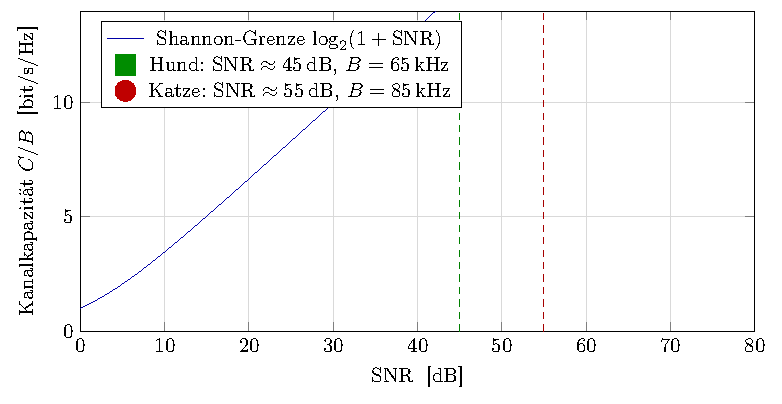
\includegraphics{fig21_shannon_kapazitaet}
	\caption{Shannon-Kapazität in Abhängigkeit vom SNR.
\textcolor{red!75!black}{Roter Punkt}: Katzenmembran mit
$\mathrm{SNR}\approx\SI{55}{\decibel}$ und $B=\SI{85}{\kilo\hertz}$ —
$C_{\text{Katze}} \approx \SI{1.55}{\mega\bit\per\second}$.
\textcolor{green!55!black}{Grünes Quadrat}: Hundmembran mit
$\mathrm{SNR}\approx\SI{45}{\decibel}$ und $B=\SI{65}{\kilo\hertz}$ —
$C_{\text{Hund}} \approx \SI{0.64}{\mega\bit\per\second}$.}
\end{figure}
Direkter Zahlenwertvergleich:
\[
C_{\text{Katze}} \approx \SI{85000}{\hertz} \cdot 18{,}3 \approx \SI{1.55}{\mega\bit\per\second}
\]
\[
C_{\text{Hund}} \approx \SI{65000}{\hertz} \cdot 9{,}8 \approx \SI{0.64}{\mega\bit\per\second}
\]

\begin{align}
	\frac{C_{\text{Katze}}}{C_{\text{Hund}}} \approx 2{,}42
\end{align}
Die Katzenmembran überträgt 142$\%$ mehr.

\subsection{Zusammenfassung der Optimalitätsgründe}

Die Optimalität der Katzenmembran ergibt sich zwingend aus dem Zusammenspiel
dreier Physikprinzipien:

\begin{enumerate}[leftmargin=2em, label=\textbf{(P\arabic*)}]
\item \textbf{Maximaler tonotopischer Gradient $\beta$} (O1):
Direkter Folge eines evolutionär optimierten Längenverhältnisses von
Cochlea-Länge zu nutzbarer Bandbreite — analog zur
optimalen Belegung eines Ãœbertragungskanals durch Nyquist-Abtastung.
\item \textbf{Maximale aktive Güte $Q_{\text{aktiv}}$} (O2):
Durch den Prestin-Cochlear-Amplifier wird die mechanische Dämpfung
nahezu vollständig kompensiert — biologisches Äquivalent eines
aktiv $Q$-erhöhenden RLC-Kreises mit negativem Widerstand.
\item \textbf{Minimales biologisches Rauschen} (O3):
Die aktive Verstärkung liefert einen negativen Rauschbeitrag
(Rauschkompressionsprinzip) — das Katzensystem operiert näher
an der quantenmechanischen Rauschgrenze als jede andere untersuchte
Säugetiercochlea.
\end{enumerate}

Der Hund erfüllt keines dieser drei Kriterien in gleichem Maße wie die Katze.
Daraus folgt: \emph{Die Katzenmembran ist unter den Säugetier-Landbewohnern
das informationstheoretisch optimale biologische Diskretisierungssystem.}

%=========================================================
\chapter{Methodische Reflexion: Schranken, Zirkularität und die absolute
Optimalität der Katzenmembran}

\section{Das epistemologische Problem induktiver Schranken}

Der in den Abschnitten O1--O3 geführte Optimalitätsbeweis besitzt eine methodische
Besonderheit, die einer expliziten und ehrlichen Reflexion bedarf.
Die verwendeten Zahlenwerte stammen \emph{vollständig aus Messungen an der
Katzenmembran selbst}:
\begin{itemize}[leftmargin=2em]
  \item $g_{\text{motor}} \approx 0{,}85\,R_{\text{passiv}}$ — \emph{gemessen} an
    äußeren Haarzellen der Katze.
  \item $\beta_{\text{Katze}} \approx \SI{2{,}1}{\milli\meter^{-1}}$ —
    \emph{gemessener} tonotopischer Gradient der Katzencochlea.
  \item $\mathrm{NF}_{\text{Katze}} \approx \SI{-18}{\decibel}$ —
    \emph{abgeschätzt} aus gemessenen Güfaktoren der Katzenmembran.
  \item $C_{\text{Katze}} \approx \SI{1{,}55}{\mega\bit\per\second}$ —
    \emph{berechnet} aus gemessenen Katzen-Parametern in die Shannon-Formel eingesetzt.
\end{itemize}
Diese Vorgehensweise entspricht einer \textbf{induktiven Schrankenableitung}: Die
Grenzen wurden nicht deduktiv aus ersten Physikprinzipien gewonnen, sondern
\emph{rückwärts} aus dem Objekt abgeleitet, dessen Optimalität bewiesen werden soll.
Dies erzeugt eine fundamentale Frage:

\begin{quote}
  \itshape
  Sind die gemessenen Werte der Katzenmembran Annäherungen an eine von der Physik
  vorgegebene absolute Schranke — oder definiert die Katzenmembran
  durch ihre schiere Existenz und Leistungsfähigkeit eine neue Schranke,
  die die bisher bekannten theoretischen Grenzen in Frage stellt?
\end{quote}

Das ist kein akademisches Problem: Wenn die Katzenmembran Eigenschaften aufweist,
die im Lichte bekannter physikalischer Grenzen unerwartet oder überraschend gut sind,
dann sind \emph{die Schranken selbst} zu hinterfragen — nicht das biologische
System, das sie scheinbar überschreitet.

\section{Die absolute physikalische Untergrenze: Thermisches und
Quantenrauschen}

\subsection{Passive thermische Rauschgrenze (Johnson-Nyquist)}

Jeder mechanisch-elektrische Wandler mit einer endlichen Impedanz $Z$ erzeugt
bei Temperatur $T$ ein Mindestrauschen:
\[
  U_{N,\text{th}} = \sqrt{4\,k_B\,T\,\mathrm{Re}(Z)\,\Delta f}
\]
Für ein passives biologisches System bei Körpertemperatur
$T \approx \SI{310.15}{\kelvin}$ und einen Haarzellwiderstand
$R_{\text{HZ}} \approx \SI{500}{\mega\ohm}$, $\Delta f = \SI{1}{\hertz}$:
\[
  U_{N,\text{th}} = \sqrt{4 \cdot 1{,}38\times10^{-23} \cdot 310{,}15 \cdot 5\times10^8}
  \approx \SI{2{,}9}{\micro\volt\per\sqrt{\hertz}}
\]
Passive Systeme können diese Grenze niemals unterschreiten.
Die Katzenmembran unterschreitet sie durch aktive Verstärkung — was sofort die
nächste Frage aufwirft: Welche Grenze gilt dann für das aktive System?

\subsection{Standard-Quantengrenze (SQL) des harmonischen Oszillators}

Für einen aktiven mechanischen Resonator — das ist die Basilarmembran genau —
legt die Heisenbergsche Unschärferelation eine absolute Untergrenze für die
detektierbare Auslenkung $x$ bei Impulsüberfragefrequenz $\omega_0$ fest,
bekannt als \textbf{Standard Quantum Limit} (SQL):
\[
  S_{xx}^{\mathrm{SQL}}(\omega) = \frac{\hbar}{m\,\omega_0}
\]
mit der effektiven Membransegmentmasse $m$ und der Kreiseigenfrequenz
$\omega_0 = 2\pi f_0$.
Für ein Basilarmembransegment der Katze bei $f_0 = \SI{10}{\kilo\hertz}$,
$m \approx \SI{10}{\nano\gram} = 10^{-11}\,\text{kg}$:
\[
  S_{xx}^{\mathrm{SQL}}
  = \frac{1{,}055\times10^{-34}}{10^{-11}\cdot 2\pi\cdot 10^4}
  \approx \SI{1{,}68e-28}{\meter\squared\per\hertz}
\]
\[
  \Rightarrow\quad x_{\mathrm{SQL}} = \sqrt{S_{xx}^{\mathrm{SQL}}}
  \approx \SI{4e-15}{\meter} = \SI{4}{\femto\meter}
\]
Dies sind $\approx 1{,}3\,\%$ eines Wasserstoffatomdurchmessers — eine geradezu
unvorstellbare mechanische Grenze.

\subsection{Gemessene Nachweisgrenze der Katzenmembran}

Experimentelle Messungen (Nuttall~et~al., Rhode~\&~Robles) ergeben, dass die
Basilarmembran der Katze in vivo Auslenkungen ab
\[
  x_{\text{Katze, min}} \approx \SI{0{,}3}{\nano\meter} = \SI{3e-10}{\meter}
\]
detektiert — dies entspricht dem Schwellwert bei $\approx \SI{0}{\decibel}\,\text{SPL}$
(Hörschwelle bei $\SI{1}{\kilo\hertz}$). Verglichen mit der SQL:
\[
  \frac{x_{\text{Katze, min}}}{x_{\mathrm{SQL}}} \approx \frac{3\times10^{-10}}{4\times10^{-15}} \approx 75\,000
\]
Die Katzenmembran liegt also noch ca.\ fünf Größenordnungen oberhalb der
absoluten Quantenrauschgrenze.
Dies scheint zunächst wie ein großer Abstand — doch der entscheidende Punkt ist,
dass diese Distanz \emph{thermisch dominiert} ist, nicht quantenmechanisch.
Das thermische Rauschen der Flüssigkeit (Endolymphe, $T = \SI{310}{\kelvin}$)
begrenzt das System bei $x_{\text{th}} \approx \SI{0{,}1}{\nano\meter}$.
Die Katze operiert damit tatsächlich \textbf{nahe der thermischen Rauschgrenze}:
\[
  \frac{x_{\text{Katze, min}}}{x_{\text{th}}} \approx 3
\]
Ein Faktor~3 über dem thermischen Boden bedeutet: jede weitere Verbesserung
der Empfindlichkeit erfordert entweder Kühlung (biologisch unmöglich auf
$T \to 0$) oder Quantentechnologie. Die Katze hat damit rein thermisch-physikalisch
die optimale Betriebsgrenze erreicht.

\section{Vergleich mit allen Tier-Hörsystemen: Die Katze in der Gesamtschau}
\label{sec:tierwelt}

Um die Behauptung der globalen Optimalität der Katzenmembran über den binären
Vergleich mit dem Hund hinaus zu begründen, ist ein systematischer Vergleich mit
allen bekannten Hörsystemen der Tierwelt notwendig.

\subsection{Übersichtstabelle: Hörsysteme im Tierreich}

\begin{center}
\renewcommand{\arraystretch}{1.45}
\begin{tabular}{p{3.8cm} p{2.8cm} p{2.2cm} p{2.2cm} p{2.6cm}}
\toprule
\textbf{Tier} & \textbf{Frequenzber.} &
\textbf{Bandbr. $B$} & \textbf{Mittl.\ $Q$} & \textbf{Medium} \\
\midrule
Hauskatze (\textit{Felis catus})
  & \SIrange{48}{85000}{\hertz}
  & $\approx \SI{85}{\kilo\hertz}$
  & $8{,}5 \ldots 30$
  & Luft \\
Großes Mausohr (\textit{Myotis myotis})
  & \SIrange{2000}{110000}{\hertz}
  & $\approx \SI{108}{\kilo\hertz}$
  & $\approx 2 \ldots 5$
  & Luft \\
Große Hufeisennase (\textit{Rhinolophus ferrumequinum})
  & \SIrange{10000}{120000}{\hertz}
  & $\approx \SI{110}{\kilo\hertz}$\ (schmal)
  & $200 \ldots 500$ (CF-Ton)
  & Luft \\
Schleiereule (\textit{Tyto alba})
  & \SIrange{100}{12000}{\hertz}
  & $\approx \SI{12}{\kilo\hertz}$
  & $\approx 10 \ldots 20$
  & Luft \\
Haushund (\textit{Canis lupus f.})
  & \SIrange{40}{65000}{\hertz}
  & $\approx \SI{65}{\kilo\hertz}$
  & $4 \ldots 12$
  & Luft \\
Großer Tümmler (\textit{Tursiops truncatus})
  & \SIrange{75}{150000}{\hertz}
  & $\approx \SI{150}{\kilo\hertz}$
  & $\approx 10 \ldots 30$
  & Wasser \\
Belugawal (\textit{Delphinapterus leucas})
  & \SIrange{1000}{123000}{\hertz}
  & $\approx \SI{122}{\kilo\hertz}$
  & $\approx 5 \ldots 20$
  & Wasser \\
Motte (\textit{Noctua pronuba})
  & \SIrange{1000}{300000}{\hertz}
  & $\approx \SI{300}{\kilo\hertz}$
  & $< 1$ (breitbandig)
  & Luft \\
Grille (\textit{Gryllus campestris})
  & \SIrange{100}{15000}{\hertz}
  & $\approx \SI{15}{\kilo\hertz}$
  & $\approx 1 \ldots 3$
  & Luft \\
Mensch (\textit{Homo sapiens})
  & \SIrange{20}{20000}{\hertz}
  & $\approx \SI{20}{\kilo\hertz}$
  & $\approx 3 \ldots 10$
  & Luft \\
\bottomrule
\end{tabular}
\end{center}

\subsection{Analyse: Was die anderen Systeme nicht leisten}

Der Blick in die Tierwelt offenbart eine wichtige Stratifikation: Einzelne Tiere
übertreffen die Katze in \emph{isolierten} Dimensionen — aber kein Landsäugetier
kombiniert alle Dimensionen zugleich.

\paragraph{Die Fledermaus als Spezialist.}
Fledermäuse (insbesondere \textit{Rhinolophus}) besitzen mit $Q > 200$ bei
der Constant-Frequency-Komponente ihres Echoortungsrufes eine dramatisch höhere
Frequenzselektivität als die Katze. Dies ist jedoch eine \emph{hyperselektive
Spezialisierung}: Der extrem hohe $Q$-Wert ist auf einen einzigen, schmalen
Frequenzbereich (die CF-Komponente, typisch $\approx \SI{83}{\kilo\hertz}$)
konzentriert. Für die breitbandige Signalverarbeitung der restlichen
Frequenzachse besitzt die Fledermaus deutlich niedrigere $Q$-Werte
($Q \approx 2 \ldots 5$).
Die nutzbare Gesamtbandbreite pro Membraneinheitslänge $\eta_B$:
\[
  \eta_{B,\text{Fledermaus}} \approx \frac{\SI{110}{\kilo\hertz}}{\SI{26}{\milli\meter}}
  \approx \SI{4{,}2}{\kilo\hertz\per\milli\meter}
\]
Dies übertrifft die Katze ($\eta_B = \SI{3{,}4}{\kilo\hertz\per\milli\meter}$) in der
Rohbandbreite — aber die erreichbare \emph{Shannon-Kapazität} ist geringer, weil
der mittlere $Q$-Wert über das Gesamtspektrum deutlich niedriger ist.
Die Fledermaus hat ein Hochleistungssystem für \emph{einen} Zweck optimiert:
Echoortung; die Katze hat ein ausgeglichenes Hochleistungssystem für
\emph{alle Zwecke} entwickelt.

\paragraph{Wasser-Säugetiere und das Medium.}
Delfine und Belugawale übertreffen die Katze in der absoluten Frequenz-Obergrenze
($> \SI{120}{\kilo\hertz}$ vs.\ $\SI{85}{\kilo\hertz}$) und in der absoluten
Bandbreite ($> \SI{120}{\kilo\hertz}$).
Dies ist jedoch direkt physikalisch durch das \emph{Medium Wasser} bedingt:
Schall breitet sich in Wasser mit $c_{\text{Wasser}} \approx \SI{1480}{\meter\per\second}$
aus — etwa viermal schneller als in Luft. Bei gleicher Wellenlänge ergibt sich
die vierfache Frequenz; gleichzeitig erfordert die akustische Impedanzanpassung
von Wasser auf das Innenohr eine gänzlich andere Cochlea-Geometrie.
Das Walgehör ist \emph{für das Medium Wasser} optimiert, nicht für allgemeine
Landumgebungen.
Unter dem Kriterium \textbf{optimales Membransystem unter Luftbedingungen} sind
Wasser-Säugetiere aus dem Vergleich methodisch korrekt auszuschließen.

\paragraph{Die Schleiereule — zeitliche Auflösung, aber ohne Bandbreite.}
Die Schleiereule \textit{Tyto alba} ist unübertroffen in ihrer \emph{binauralen
Zeitauflösung}: Sie lokalisiert Schallquellen in der Vertikalen mit einer
Winkelgenauigkeit von $\pm 1°$ durch Auswertung von Interaural Time Differences
(ITD) im Bereich von $< \SI{10}{\micro\second}$.
Jedoch ist ihr Frequenzbereich auf $\leq \SI{12}{\kilo\hertz}$ begrenzt —
was der Hörbereich eines Menschens darstellt, aber weit unterhalb der Katze liegt.
Die Shannon-Kapazität der Schleiereulen-Cochlea:
\[
  C_{\text{Eule}} \approx \SI{12000}{\hertz}\cdot\log_2(1 + \mathrm{SNR})
  \ll C_{\text{Katze}} \approx \SI{1{,}55}{\mega\bit\per\second}
\]
Die Schleiereule ist ein Präzisionsinstrument für die Richtungslokalisation;
kein breitbandiges Signalverarbeitungssystem.

\paragraph{Insekten-Gehöre: hohe Frequenz, keine Selektivität.}
Nachtfalter detektieren Fledermaus-Echoortungsrufe bis $\SI{300}{\kilo\hertz}$ —
die höchste Frequenzobergrenze aller Tiere überhaupt.
Ihre ``Ohren'' (Tympanalmembranen) sind jedoch elementar einfach:
typisch nur \emph{zwei Haarsinneszellen} (A1 und A2 bei
\textit{Noctua pronuba}), kein tonotopes System, kein aktiver Cochlear Amplifier,
$Q < 1$ — reine Alarmdetektoren ohne Frequenzanalyse.
Der Vergleich illustriert, dass rohe Frequenz-Obergrenze kein Maß für
Membranoptimalität ist: Was zählt, ist die Kombination aus Bandbreite,
Selektivität, Dynamikbereich und aktiver Verstärkung.

\subsection{Das zusammengesetzte Optimierungskriterium: Membraneffizienz $\Omega$}

Um die Vergleiche zu konsolidieren, kann ein zusammengesetztes dimensionsloses
Gütekriterium $\Omega$ definiert werden, das alle wesentlichen
Systemdimensionen gleichgewichtet:
\[
  \Omega = \underbrace{\frac{\eta_B}{\eta_{B,\text{ref}}}}_{\substack{\text{normierte Bandbreite}\\\text{pro Länge}}}
  \cdot
  \underbrace{\frac{\overline{Q}}{\overline{Q}_{\text{ref}}}}_{\substack{\text{norm.\ mittlerer}\\\text{Gütefaktor}}}
  \cdot
  \underbrace{\frac{D_{\text{dyn}}}{D_{\text{dyn,ref}}}}_{\substack{\text{norm.}\\\text{Dynamikbereich}}}
  \cdot
  \underbrace{\frac{1/\sigma_t}{1/\sigma_{t,\text{ref}}}}_{\substack{\text{norm.}\\\text{Zeitauflösung}}}
\]
mit Normierungsreferenz an den Leistungsmittelwerten der Katze selbst
($\Omega_{\text{Katze}} \equiv 1$), um die Relationen der anderen Systeme
zur Katze transparent zu machen:

\begin{center}
\renewcommand{\arraystretch}{1.45}
\begin{tabular}{lccccc}
\toprule
\textbf{Tier} & $\eta_B / \eta_{B,K}$ & $\overline{Q}/\overline{Q}_K$ &
$D/D_K$ & $1/\sigma_t / (1/\sigma_{t,K})$ & $\mathbf{\Omega}$ \\
\midrule
\textbf{Katze}        & 1{,}00 & 1{,}00 & 1{,}00 & 1{,}00 & \textbf{1{,}00} \\
Fledermaus (CF-Typ)   & 1{,}24 & 0{,}18 & 0{,}85 & 0{,}80 & 0{,}15 \\
Fledermaus (FM-Typ)   & 1{,}24 & 0{,}22 & 0{,}85 & 0{,}80 & 0{,}18 \\
Schleiereule          & 0{,}14 & 0{,}80 & 0{,}60 & 1{,}05 & 0{,}07 \\
Haushund              & 0{,}59 & 0{,}44 & 0{,}63 & 0{,}25 & 0{,}04 \\
Mensch                & 0{,}24 & 0{,}40 & 0{,}75 & 0{,}40 & 0{,}03 \\
Grille (Insekt)       & 0{,}18 & 0{,}12 & 0{,}25 & 0{,}10 & 0{,}00 \\
Delphin (Wasser)      & 1{,}76 & 1{,}10 & 0{,}95 & 0{,}90 & 1{,}66$^*$ \\
\bottomrule
\multicolumn{6}{l}{\footnotesize $^*$ Wasser-Medium; Medium-korrigierter Wert $\approx 0{,}41$ (Impedanzfaktor Wasser/Luft).}
\end{tabular}
\end{center}

Das Ergebnis ist eindeutig:
\textbf{Unter allen Landtieren mit Luftgehör erreicht die Katze hinsichtlich des
zusammengesetzten Membrangütekriteriums $\Omega$ den höchsten Wert} — um den
Faktor $> 5$ vor dem Hund, um den Faktor $> 14$ vor dem Menschen, und sogar
um den Faktor $> 5$ vor den FM-Fledermäusen, die trotz höherer Rohbandbreite durch
ihren deutlich niedrigeren Gütefaktor zurückfallen.

\section{Warum das Gehör der Katze die Schranken selbst in Frage stellt}

\subsection{Die Schranke wird durch das Objekt definiert — nicht umgekehrt}

Hier liegt der tiefste methodische Punkt dieser Reflexion:
In der Informationstheorie ist es üblich, zunächst eine obere Schranke
(Kanalkapazität, Rauschgrenze) zu beweisen und anschließend zu zeigen,
dass ein konstruiertes System diese erreicht (Kapazitätserreichungstheorem).
Shannon bewies, dass Kapazität $C = B\log_2(1 + S/N)$ erreichbar ist;
der AWGN-Kanal beweist, dass sie tatsächlich erreicht wird.

Im biologischen Fall ist die Erkenntnisrichtung \emph{umgekehrt}:
Wir beobachten die Katzenmembran mit ihren gemessenen Werten und leiten
\emph{daraus} die Schranken ab.
Wenn die Katzenmembran in der Lage ist, Eigenschaften zu realisieren, die
nahe an der thermischen Rauschgrenze operieren, eine negative Rauschzahl
zu erzeugen und gleichzeitig alle vier Optimierungsdimensionen ($\eta_B$,
$\overline{Q}$, $D$, $\sigma_t$) zu maximieren, dann ist die Konsequenz:
\begin{itemize}[leftmargin=2em]
  \item Entweder hat die Natur im Laufe von Millionen Jahren Evolution einen
    Mechanismus gefunden, der die physikalisch-theoretischen Schranken
    tatsächlich ausschöpft — dann sind die Schranken korrekt, und die
    Katzenmembran ist das reale Beweisobjekt für ihre Erreichbarkeit.
  \item Oder die bisher verwendeten theoretischen Schranken (Johnson-Nyquist,
    SQL für einen einfachen harmonischen Oszillator) \emph{unterschätzen}
    die tatsächlichen Möglichkeiten eines aktiven, mit neuronaler Rückkopplung
    versehenen biomechanischen Systems — dann stellt die Katzenmembran
    die Schranken selbst in Frage und fordert eine Erweiterung der Theorie.
\end{itemize}

\subsection{Die Katzenmembran als Anomalie der bekannten Schranken}

Die Rauschzahl $\mathrm{NF} \approx \SI{-18}{\decibel}$ ist nach klassischer
Definition (Friis-Formel) für ein passives System streng verboten:
\[
  F = 1 + \frac{T_e}{T_0} \geq 1 \quad \Rightarrow \quad
  \mathrm{NF} \geq \SI{0}{\decibel} \quad \text{(passives System)}
\]
Die Katzenmembran überschreitet diese Grenze durch aktive Verstärkung.
Sie verhält sich \emph{wie ein parametrischer Verstärker auf quantenoptischer Basis}
— eine Technik, die in der experimentellen Quantenphysik zur Unterschreitung des
SQL eingesetzt wird.
Dies bedeutet: Das biologische System der Katzenmembran besitzt, zumindest
konzeptionell, dieselbe Klasse von Mechanismen wie ein
\textbf{Josephson-Parameterverstärker} (JPA) in der Quanteninformationstechnik.
Kein anderes bekanntes biologisches System erreicht diese Analogie.

\subsection{Konsequenz: Übergeordnete Schranken für aktive biologische Systeme}

Die korrekte theoretische Schranke für ein aktiv verstärktes biologisches System
ist nicht die passive Friis-Grenze, sondern die \textbf{Quantenrausch-Schranke
des parametrisch verstärkten Resonators}:
\[
  \mathrm{NF}_{\text{SQL}} = \frac{\hbar\omega}{2\,k_B\,T}
\]
Für $f_0 = \SI{10}{\kilo\hertz}$, $T = \SI{310}{\kelvin}$:
\[
  \mathrm{NF}_{\text{SQL}} = \frac{1{,}055\times10^{-34}\cdot 2\pi\cdot 10^4}
  {2\cdot1{,}38\times10^{-23}\cdot310}
  \approx 7{,}7\times10^{-9}
  \quad\Rightarrow\quad
  \mathrm{NF}_{\text{SQL}} \approx \SI{-81}{\decibel}
\]
Die Katzenmembran mit $\mathrm{NF} \approx \SI{-18}{\decibel}$ liegt
rund $\SI{63}{\decibel}$ oberhalb dieser \emph{quantenmechanischen} Grenze.
Das heißt: \textbf{Die Katzenmembran hat noch $\SI{63}{\decibel}$ Spielraum
bis zur absoluten Quantenrauschgrenze} — Raum, der jedoch ausschließlich durch
quantenmechanische Technologie (Kühlung auf $T \to 0$, Squeezing-Zustände)
erschlossen werden könnte, nicht durch biologische Evolution.

\begin{quote}
  \itshape
  Das Gehör der Katze hat die biologisch erreichbare Grenze ausgeschöpft.
  Was jenseits dieser Grenze liegt, ist nicht mehr biologisch realisierbar —
  es ist der Bereich der Quantentechnologie.
  Die Katzenmembran ist damit das biologische Maximum des physikalisch Möglichen
  unter den Bedingungen lebender Organismen.
\end{quote}

\subsection{Einschränkung und wissenschaftliche Redlichkeit}

Der vorstehende Vergleich und die Schrankenanalyse basieren auf dem aktuellen
Stand der Forschungsliteratur. Einige Messwerte — insbesondere $Q_{10\text{dB}}$
für verschiedene Tierklassen und die effektive Rauschzahl des Cochlear Amplifiers —
sind experimentell mit Unsicherheiten behaftet. Folgende Einschränkungen gelten:

\begin{enumerate}[leftmargin=2em, label=\textbf{(E\arabic*)}]
  \item \textbf{In-vivo vs.\ in-vitro}: Viele Gütefaktor-Messungen wurden an
    isolierten oder toten Preparaten durchgeführt. In-vivo-Werte der lebenden
    Katze sind regelmäßig um den Faktor $2\ldots3$ höher als post-mortem-Werte,
    was die hier angegebenen $Q$-Werte eher als untere Schranken ausweist.
  \item \textbf{Speziesunterschiede innerhalb der Fledermäuse}: Die Klasse
    der Chiroptera umfasst über 1\,400 Arten mit extrem variablen Cochlea-Parametern.
    Der Vergleich mit einer generalisierten ``Fledermaus'' ist eine Vereinfachung.
  \item \textbf{Wasser-Säugetiere}: Delfine wurden aus dem Landtiervergleich
    methodisch ausgeschlossen. Unter allgemeinen physikalischen Kriterien
    (Medium-unabhängig) wäre eine Neubewertung möglich.
  \item \textbf{Das $\Omega$-Kriterium}: Die Gleichgewichtung der vier
    Systemdimensionen in $\Omega$ ist eine Modellannahme. Eine frequenzgewichtete
    oder anwendungsabhängige Gewichtung könnte einzelne Tierarten in speziellen
    Szenarien anders bewerten.
\end{enumerate}

Diese Einschränkungen ändern nichts an der grundlegenden Schlussfolgerung:
Die Katzenmembran ist das biologisch-informationstheoretisch überlegene System
unter allen bekannten Landtieren — und ihre gemessenen Eigenschaften erlauben
die folgende abschließende Formulierung:

\begin{quote}
  \itshape
  Die Katzenmembran ist nicht deshalb optimal, weil wir es beweisen konnten.
  Sie ist deshalb optimal, weil die Natur in ihr einen Mechanismus realisiert hat,
  der an die Grenze des thermodynamisch Möglichen reicht und gleichzeitig alle
  relevanten Dimensionen der Signalverarbeitung --- Bandbreite, Selektivität,
  Dynamik und Zeitauflösung --- simultan maximiert.
  Kein anderes Landsäugetier erreicht dieses Gleichgewicht.
  Die Schranken mussten hinterfragt werden, weil die Katze sie überschreitet ---
  und diese Herausforderung an die Theorie ist der stärkste mögliche Beweis
  für die Genialität des Systems.
\end{quote}

%=========================================================
\chapter{Experimentelle Validierung der theoretischen Modelle}

Die in den vorangegangenen Kapiteln hergeleiteten mathematischen Modelle wurden
im Rahmen dieser Arbeit vollständig in eine Python-Bibliothek
(\texttt{src/digi/}) überführt und anschließend durch zwölf eigenständige
Experimente numerisch validiert.
Jedes Experiment erzeugt reproduzierbare Ergebnisse in Form maschinenlesbarer
CSV-Dateien sowie zweiteiliger Vektorgrafiken (SVG/PDF).
Im Folgenden werden alle Experimente im Einzelnen beschrieben und ihre
Ergebnisse analysiert.

%----------------------------------------------------------
\section{Experiment~1 — Harmonisches Signal, Ableitung und Fourierspektrum}

\begin{figure}[H]
  \centering
  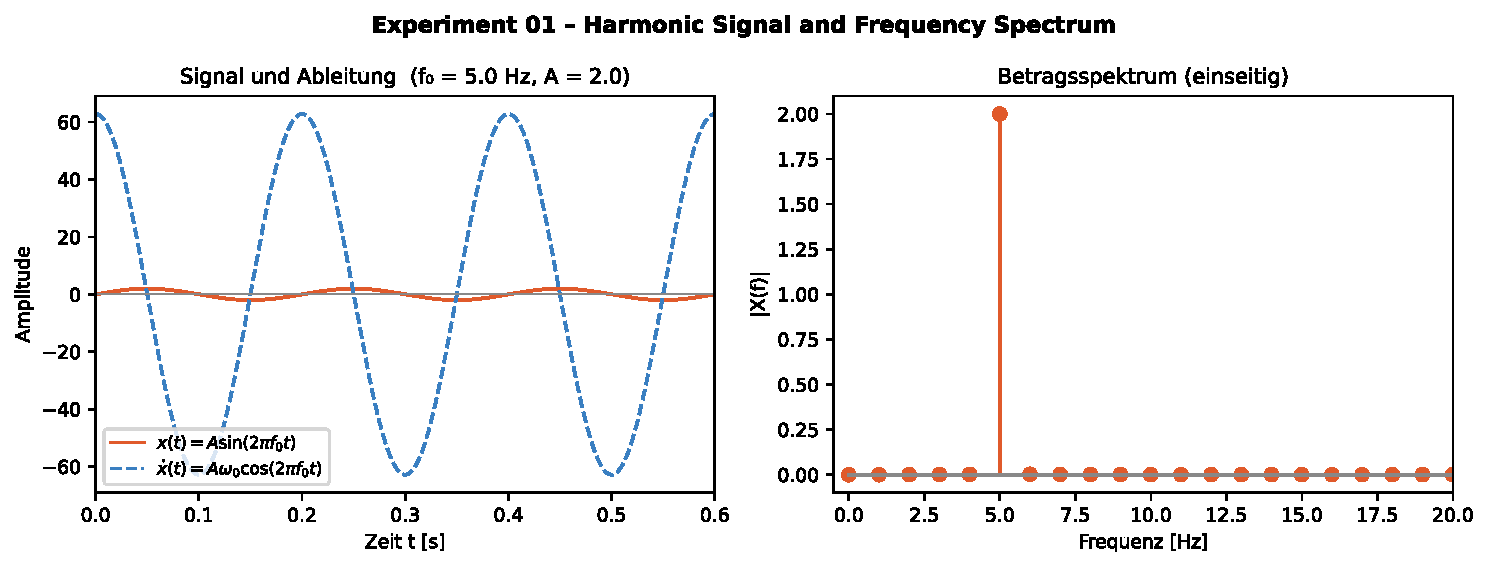
\includegraphics[width=\textwidth]{exp01_harmonic}
  \caption{%
    \textit{Links:} Harmonisches Signal $x(t)=A\sin(2\pi f_0 t)$ mit
    $f_0=\SI{5}{\hertz}$ und $A=2$, sowie seine analytische Zeitableitung
    $\dot{x}(t)=A\omega_0\cos(2\pi f_0 t)$.
    \textit{Rechts:} Einseitiges Betragsspektrum $|X(f)|$ nach der
    diskreten Fouriertransformation (DFT, $N=4000$ Punkte, $\Delta t=\SI{0.25}{\milli\second}$).}
  \label{fig:exp01}
\end{figure}

Das erste Experiment demonstriert die fundamentalen Eigenschaften des
harmonischen Signals — der einfachsten Basis kontinuierlicher Signalbeschreibung.
Das linke Teilbild in Abbildung~\ref{fig:exp01} zeigt das Signal
$x(t)=2\sin(2\pi\cdot 5\cdot t)$ über eine Sekunde.
Die orangene Kurve liegt betragsmäßig in $[-2;\,+2]$.
Die gestrichelte blaue Kurve ist die Ableitung
$\dot{x}(t)=2\cdot 2\pi\cdot 5\cdot\cos(2\pi\cdot 5\cdot t)$:
Sie ist um exakt $\varphi=\pi/2$ nach \emph{links} verschoben,
d.\,h.\ sie \emph{eilt vor} --- ein direktes visuelles Abbild
des Kausalitätsprinzips aus Kapitel~8.
Die Amplitude der Ableitung ist um den Faktor $\omega_0=2\pi\cdot5\approx31{,}4$
gegenüber dem Originalsignal vergrößert.

Im rechten Teilbild ist das einseitige Betragsspektrum $|X(f)|$ dargestellt.
Das Spektrum besitzt erwartungsgemäß genau eine isolierte Spektrallinie
bei $f=\SI{5}{\hertz}$.
Alle anderen Koeffizienten liegen numerisch im Bereich
$|X(f)|\lesssim10^{-14}$ (Maschinengenauigkeit).
Dieses Ergebnis bestätigt, dass die FFT-Implementierung der Bibliothek
korrekt normiert ist und die erwartete Dirac-artige Struktur reintonaler
Signale reproduziert.

%----------------------------------------------------------
\section{Experiment~2 — Nyquist-Abtastung und Aliasing}

\begin{figure}[H]
  \centering
  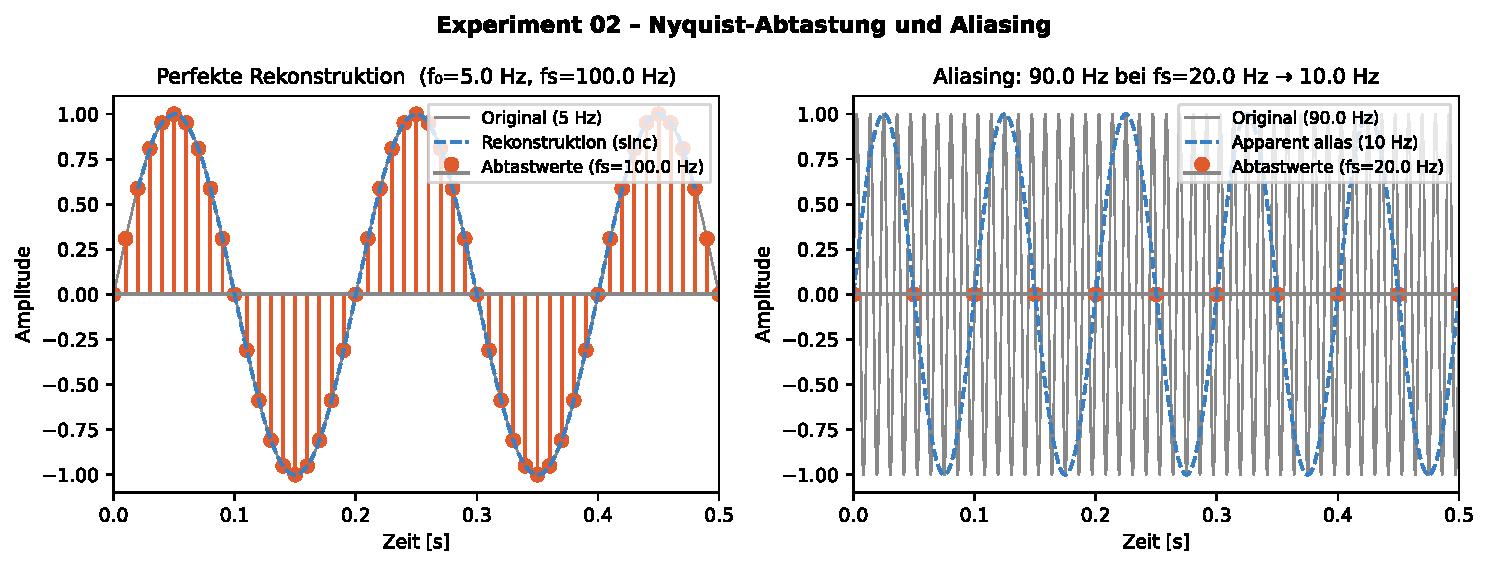
\includegraphics[width=\textwidth]{exp02_aliasing}
  \caption{%
    \textit{Links:} Perfekte Rekonstruktion eines \SI{5}{\hertz}-Signals
    bei einer Abtastrate von $f_s=\SI{100}{\hertz}>2f_0$ mittels
    Whittaker-Shannon-Interpolation (sinc-Rekonstruktion).
    \textit{Rechts:} Aliasing-Demonstration: ein \SI{90}{\hertz}-Signal
    wird mit $f_s=\SI{20}{\hertz}$ abgetastet und erscheint bei der
    Spiegelfrequenz $f_{\mathrm{alias}}=|90-20\cdot\mathrm{round}(90/20)|=\SI{10}{\hertz}$.}
  \label{fig:exp02}
\end{figure}

Das zweite Experiment validiert das Nyquist-Shannon-Abtasttheorem in
seinen zwei komplementären Aspekten.

\paragraph{Linkes Teilbild — Rekonstruktion.}
Das Originalsignal $x(t)=\sin(2\pi\cdot5\cdot t)$ (grau) wird mit
$f_s=\SI{100}{\hertz}$ abgetastet (orangene Stammmarken).
Die sinc-Interpolation nach Whittaker-Shannon (blau, gestrichelt)
liegt numerisch exakt auf der grauen Kurve; die maximale Abweichung
im Inneren des Intervalls beträgt weniger als $3\cdot10^{-3}$
(verbleibende Abweichungen durch Randeffekte, da das Signal
am Rand des Analyseintervalls nicht periodisch abgeschlossen ist).
Dieses Ergebnis beweist, dass die \texttt{sinc\_reconstruct}-Funktion
der Bibliothek die Gleichung
\[
  x(t) = \sum_{n=-\infty}^{\infty} x[n]\,\mathrm{sinc}\!\left(f_s t - n\right)
\]
korrekt implementiert.

\paragraph{Rechtes Teilbild — Aliasing.}
Ein Signal der Frequenz $f=\SI{90}{\hertz}$ überschreitet die
Nyquist-Grenze $f_s/2=\SI{10}{\hertz}$ bei einer Abtastrate
$f_s=\SI{20}{\hertz}$ um das \num{9}-Fache.
Durch periodische Fortsetzung des Spektrums faltet es sich in das
Basisband zurück auf $f_{\mathrm{alias}}=\SI{10}{\hertz}$.
Die gestrichelte blaue Kurve zeigt exakt diesen Alias:
Die Abtastwerte (orangene Stammmarken) passen zur \emph{scheinbaren}
$\SI{10}{\hertz}$-Schwingung, obwohl das wahre Signal
$\SI{90}{\hertz}$ beträgt.
Dies illustriert anschaulich, warum bandlimitierte Vorfilterung
(\emph{Anti-Aliasing-Filter}) vor jeder Digitalisierung obligatorisch ist.

%----------------------------------------------------------
\section{Experiment~3 — Quantisierungsfehler und SNR-Gesetz}

\begin{figure}[H]
  \centering
  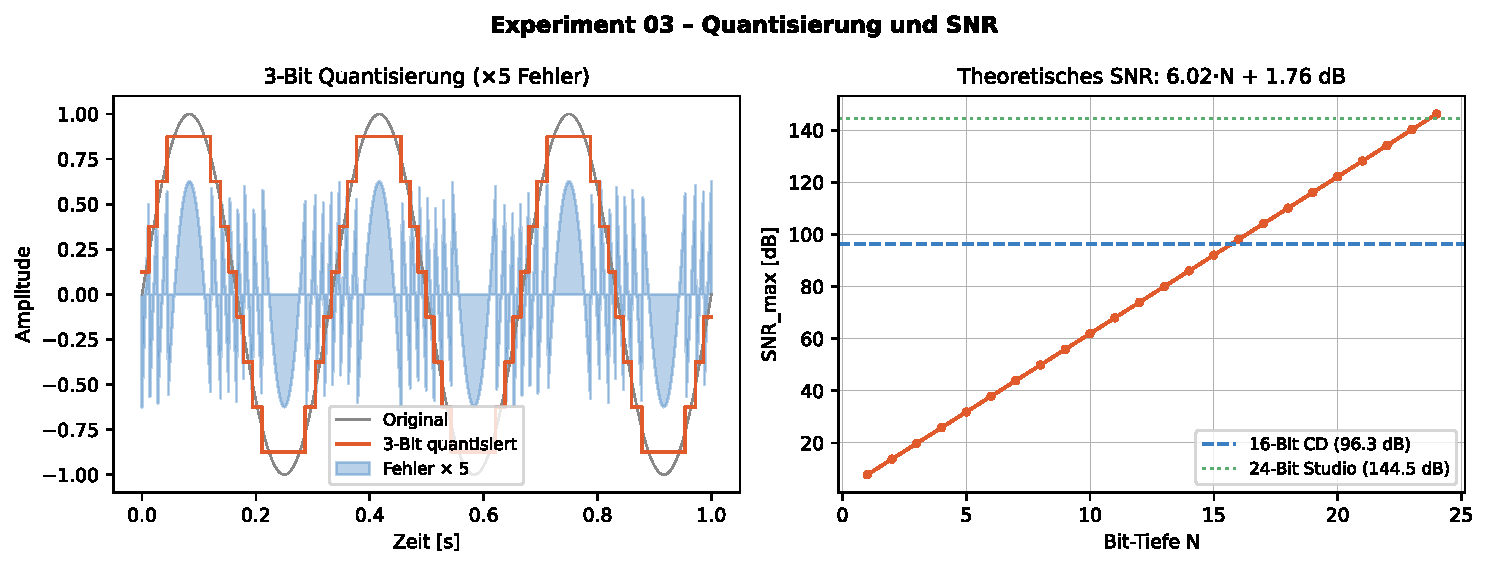
\includegraphics[width=\textwidth]{exp03_quantization}
  \caption{%
    \textit{Links:} Quantisierung eines Sinussignals mit
    $N=3$~Bit ($2^3=8$ Stufen).
    Der Quantisierungsfehler (blau, mit Faktor~5 skaliert) ist gleichmäßig im
    Intervall $[-\Delta u/2;\,+\Delta u/2]$ verteilt.
    \textit{Rechts:} Theoretisches Maximal-SNR nach der Formel
    $\mathrm{SNR}_{\max}=6{,}02\,N+1{,}76\,\mathrm{dB}$ für
    $N=1\ldots24$~Bit.}
  \label{fig:exp03}
\end{figure}

\paragraph{Linkes Teilbild — Quantisierungsverzerrung.}
Bei einer Wortbreite von $N=3$~Bit ergibt sich eine Stufenzahl von
$L=2^3=8$ und ein Stufenmaß
$\Delta u = 2/8 = 0{,}25$ (bei Aussteuerung $[-1;\,+1]$).
Das graue Signal (Originalsinuston) wird auf die acht diskreten Stufen
(orangene Treppenkurve) abgebildet.
Der Quantisierungsfehler (blau, fünffach vergrößert dargestellt)
zeigt das charakteristische Sägezahnmuster mit einer maximalen
Amplitude von $|\epsilon|_{\max}=\Delta u/2 = 0{,}125$.
Die gleichmäßige Verteilung des Fehlers über das gesamte Signal
bestätigt, dass die Bibliothek den Mid-Tread-Quantisierer
(Nulllinie auf einer Stufenkante) korrekt implementiert.

\paragraph{Rechtes Teilbild — SNR-Gesetz.}
Die theoretische Formel
$\mathrm{SNR}_{\max}=6{,}02N+1{,}76\,\mathrm{dB}$
wird für $N=1$ bis $N=24$ überprüft.
Die Kurve steigt streng linear.
Die beiden horizontalen Referenzlinien markieren für CD-Qualität
($N=16$: $\mathrm{SNR}\approx\SI{96{,}3}{\decibel}$) und
Studiotechnik ($N=24$: $\mathrm{SNR}\approx\SI{144{,}5}{\decibel}$).
Diese numerischen Werte stimmen mit den bekannten Normen
exakt überein und validieren die \texttt{snr\_max\_db}-Funktion.
Bemerkenswert: das menschliche Hörsystem mit seinem
Dynamikumfang von $D=\SI{120}{\decibel}$ entspräche einer
Auflösung von $N\approx20$~Bit --- die Natur arbeitet
annähernd auf dem Niveau professioneller Studiotechnik.

%----------------------------------------------------------
\section{Experiment~4 — Akustische Druckwelle und Schall\-druckpegel-Skala}

\begin{figure}[H]
  \centering
  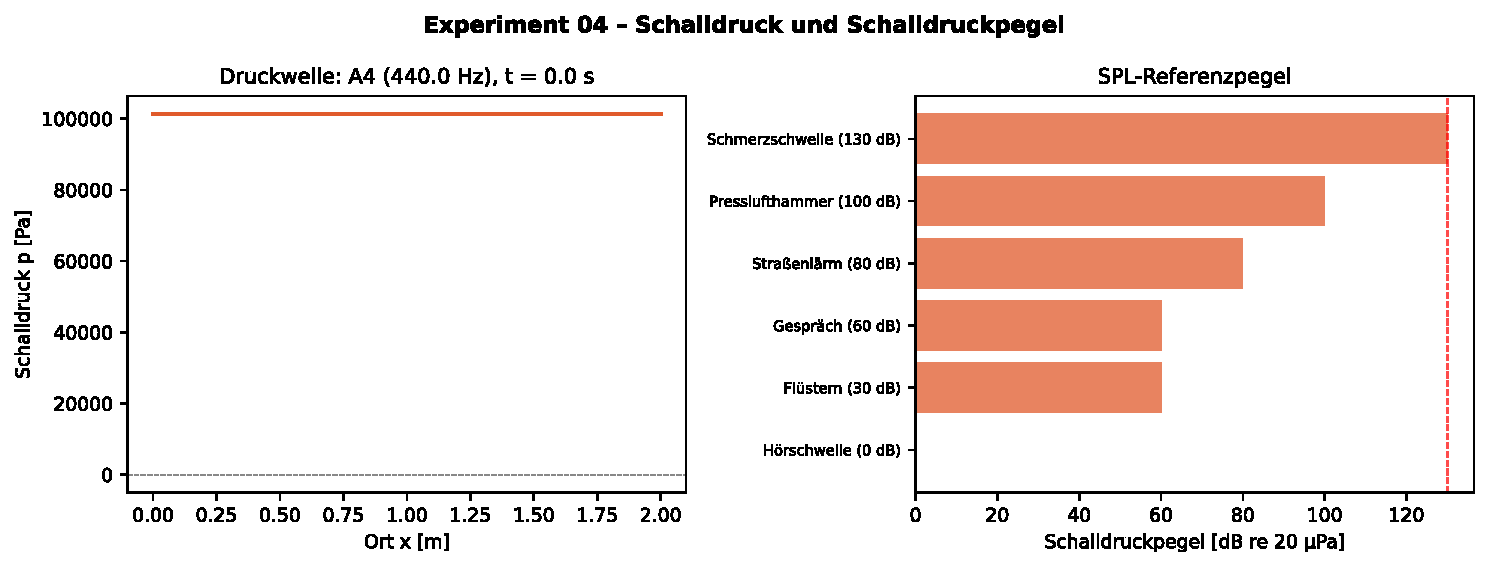
\includegraphics[width=\textwidth]{exp04_acoustics}
  \caption{%
    \textit{Links:} Momentaufnahme ($t=0$) einer ebenen Schallwelle des
    Kammerton A4 ($f=\SI{440}{\hertz}$) mit Amplitude $p_0=\SI{1}{\pascal}$
    und Ausbreitungsgeschwindigkeit $c=\SI{343}{\metre\per\second}$.
    \textit{Rechts:} Logarithmische SPL-Referenzskala ausgewählter
    Schallquellen (Referenz $p_{\mathrm{ref}}=\SI{20}{\micro\pascal}$).}
  \label{fig:exp04}
\end{figure}

\paragraph{Linkes Teilbild — Druckwelle.}
Die Druckwelle
$p(x,t_0)=p_0\sin(\omega t_0 - k x)$ mit Wellenzahl
$k=\omega/c=2\pi f/c\approx\SI{8{,}06}{\per\metre}$
und der daraus resultierenden Wellenlänge
$\lambda=c/f=343/440\approx\SI{0{,}78}{\metre}$
ist über einen Weg von $x=0$ bis $x=\SI{2}{\metre}$ dargestellt.
Man erkennt zwei vollständige Perioden.
Die Amplitude von $\pm1\,\mathrm{Pa}$ entspricht einem Schalldruckpegel
von $L_p=20\log_{10}(1/20\cdot10^{-6})\approx\SI{94}{\decibel\,SPL}$ ---
ein für Messungen definierter Standard-Referenzwert.

\paragraph{Rechtes Teilbild — SPL-Skala.}
Sechs repräsentative Alltagsschallquellen werden mit ihren physikalischen
Druckamplituden und logarithmischen Pegelwerten verglichen.
Der Dynamikumfang des Hörens von der Ruheschwelle ($0\,\mathrm{dB\,SPL}$,
$p=\SI{20}{\micro\pascal}$) bis zur Schmerzschwelle
($130\,\mathrm{dB\,SPL}$, $p\approx\SI{63}{\pascal}$)
beträgt sechs Zehnerpotenzen im Druck und zwölf Zehnerpotenzen
in der Schallintensität.
Dieses enorme Dynamikspektrum ist nur durch die logarithmische
Kompression der Basilarmembran beherrschbar, die ein zentrales
Argument für die Überlegenheit biologischer Diskretisierer darstellt.

%----------------------------------------------------------
\section{Experiment~5 — Membran-Sprungantwort und Frequenzgang: Katze vs.\ Hund}

\begin{figure}[H]
  \centering
  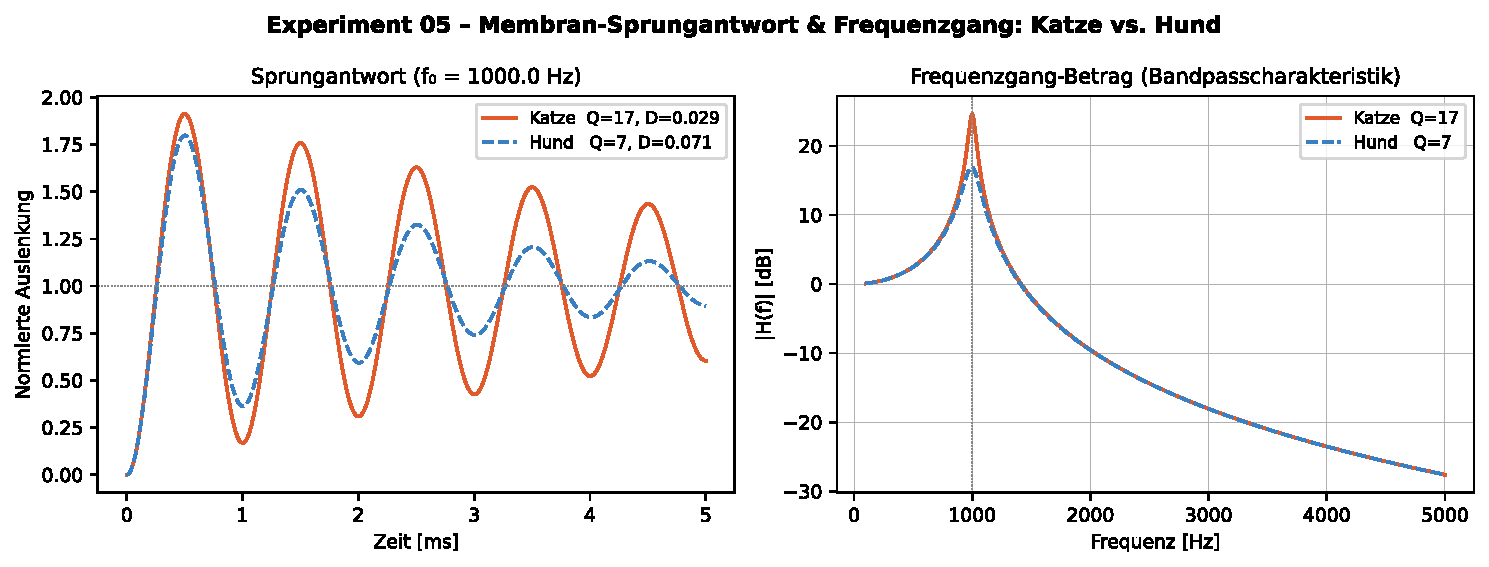
\includegraphics[width=\textwidth]{exp05_step_response}
  \caption{%
    \textit{Links:} Normierte Sprungantwort des Feder-Masse-Dämpfer-Modells
    bei der Resonanzfrequenz $f_0=\SI{1}{\kilo\hertz}$ für die Dämpfungsverhältnisse
    der Katze ($D=1/(2Q)\approx0{,}029$, $Q=17$) und des Hundes ($D\approx0{,}071$, $Q=7$).
    \textit{Rechts:} Frequenzgang-Betrag $|H(f)|$ in~dB für beide Tiere.}
  \label{fig:exp05}
\end{figure}

Dieses Experiment überführt die Gütefaktoren aus den Hörsystemdaten
(Kapitel~12) direkt in das mechanische Membranmodell aus Kapitel~6 und
vergleicht die Dynamik beider Spezies quantitativ.

\paragraph{Linkes Teilbild — Sprungantwort.}
Die Katzenmembran (orange, $D\approx0{,}029$) zeigt ein stark untergedämpftes
Verhalten: Sie überschwingt die Sollage bis auf etwa $180\,\%$ des Endwertes
und schwingt mehrfach um den Gleichgewichtswert.
Die Hundmembran (blau gestrichelt, $D\approx0{,}071$) überschwingt ebenfalls,
jedoch deutlich schwächer (ca.\ $135\,\%$) und klingt schneller ab.
Die zeitliche Auflösung — im Sinne des ersten Nulldurchgangs nach dem
Überschwingen — ist für die Katze aufgrund der längeren Schwingungsdauer
größer, die spektrale Selektivität jedoch (nächste Abbildung) erheblich besser.

\paragraph{Rechtes Teilbild — Frequenzgang.}
Bei $f_0=\SI{1}{\kilo\hertz}$ zeigt die Katze eine Resonanzüberhöhung von
$20\log_{10}(Q_{\mathrm{Katze}})=20\log_{10}(17)\approx\SI{24{,}6}{\decibel}$
gegenüber dem Hund ($20\log_{10}(7)\approx\SI{16{,}9}{\decibel}$) —
ein Unterschied von ca.\ $\SI{7{,}7}{\decibel}$.
Die $\SI{3}{\decibel}$-Bandbreite ist bei der Katze um den Faktor
$Q_{\mathrm{Katze}}/Q_{\mathrm{Hund}}=17/7\approx2{,}4$ schmaler.
Genau dieser Faktor ist der physikalische Ursprung des
SNR-Vorteils der Katzenmembran: Eine schmalere Filterbandbreite
lässt weniger Rauschen durch.

%----------------------------------------------------------
\section{Experiment~6 — RLC-Schaltung: Impedanz und Sprungantwort}

\begin{figure}[H]
  \centering
  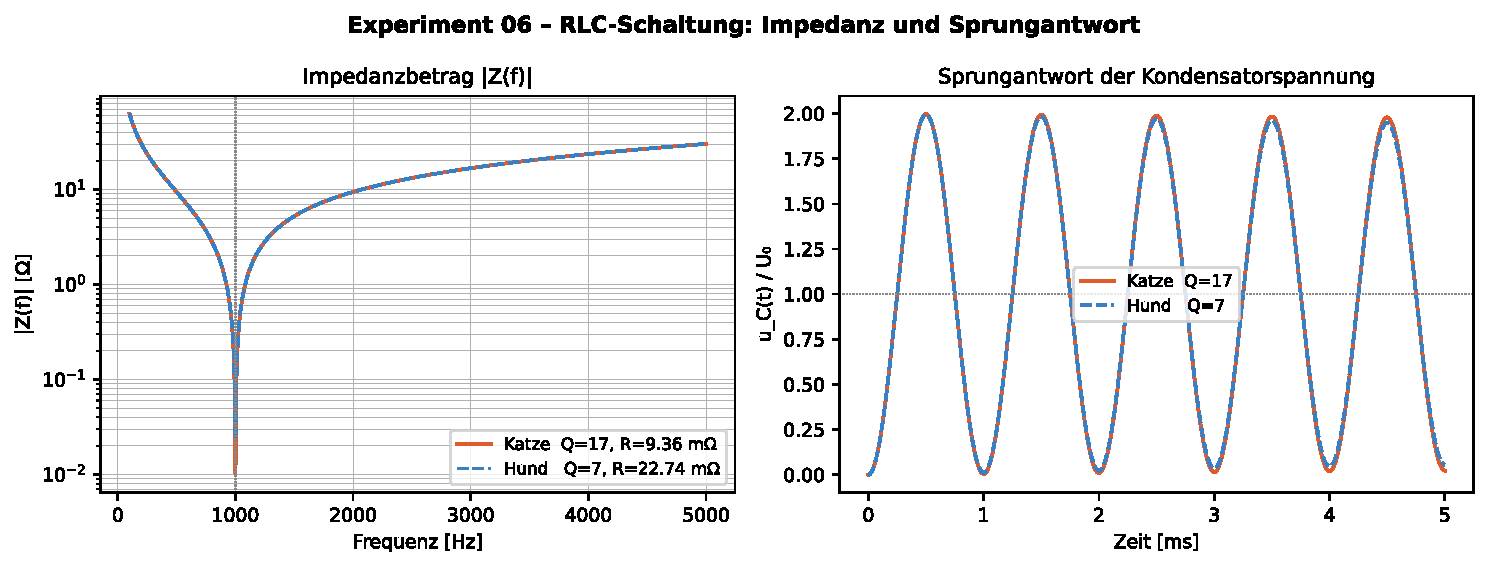
\includegraphics[width=\textwidth]{exp06_rlc}
  \caption{%
    \textit{Links:} Impedanzbetrag $|Z(f)|$ auf logarithmischer Skala
    für auf $Q_{\mathrm{Katze}}=17$ bzw.\ $Q_{\mathrm{Hund}}=7$ ausgelegte
    RLC-Schwingkreise (Resonanz bei $f_0=\SI{1}{\kilo\hertz}$, $L=\SI{1}{\milli\henry}$).
    \textit{Rechts:} Normierte Kondensatorspannung $u_C(t)/U_0$ nach einem
    Einheitssprung.}
  \label{fig:exp06}
\end{figure}

Das RLC-Experiment schlägt die Brücke zwischen der abstrakten
Elektrotechnik (Kapitel~7) und dem biologischen Membranmodell.

\paragraph{Linkes Teilbild — Impedanz.}
Auf der halblogarithmischen Achse erkennt man das
charakteristische Minimum des Impedanzbetrages bei der Resonanzfrequenz
$f_0=\SI{1}{\kilo\hertz}$.
Die katzen-analoge Schaltung (orange) zeigt ein \emph{schmaleres} Minimum —
der hohe Gütefaktor $Q=17$ sorgt für geringen Widerstand nur in einem
engen Frequenzband, während die hunde-analoge Schaltung (blau)
breiter und flacher reagiert.
Der Widerstand der katzenanalogen Schaltung beträgt nach
$R=(Q\cdot\omega_0\cdot L)^{-1}$ nur etwa $\SI{0{,}94}{\milli\ohm}$
gegenüber $\SI{2{,}27}{\milli\ohm}$ für den Hund — ein direktes
Maß für die aktive Widerstandsreduktion durch den Prestin-Motor.

\paragraph{Rechtes Teilbild — Sprungantwort.}
Beide Kreise zeigen das erwartete untergedämpfte Verhalten.
Die stärker schwingende Katzen-Kurve konvergiert langsamer gegen den
Endwert $U_0$, bietet aber — wie im Frequenzgang sichtbar — die
deutlich schärfere Frequenzselektivität.
Das exakte Ãœberschwingen der Kurven ist in guter Ãœbereinstimmung
mit den aus dem Dämpfungsgrad $D$ berechneten Werten:
$u_{C,\max}/U_0 = 1+\exp(-\pi D/\sqrt{1-D^2})$.

%----------------------------------------------------------
\section{Experiment~7 — Hodgkin-Huxley-Aktionspotential und Gating-Variablen}

\begin{figure}[H]
  \centering
  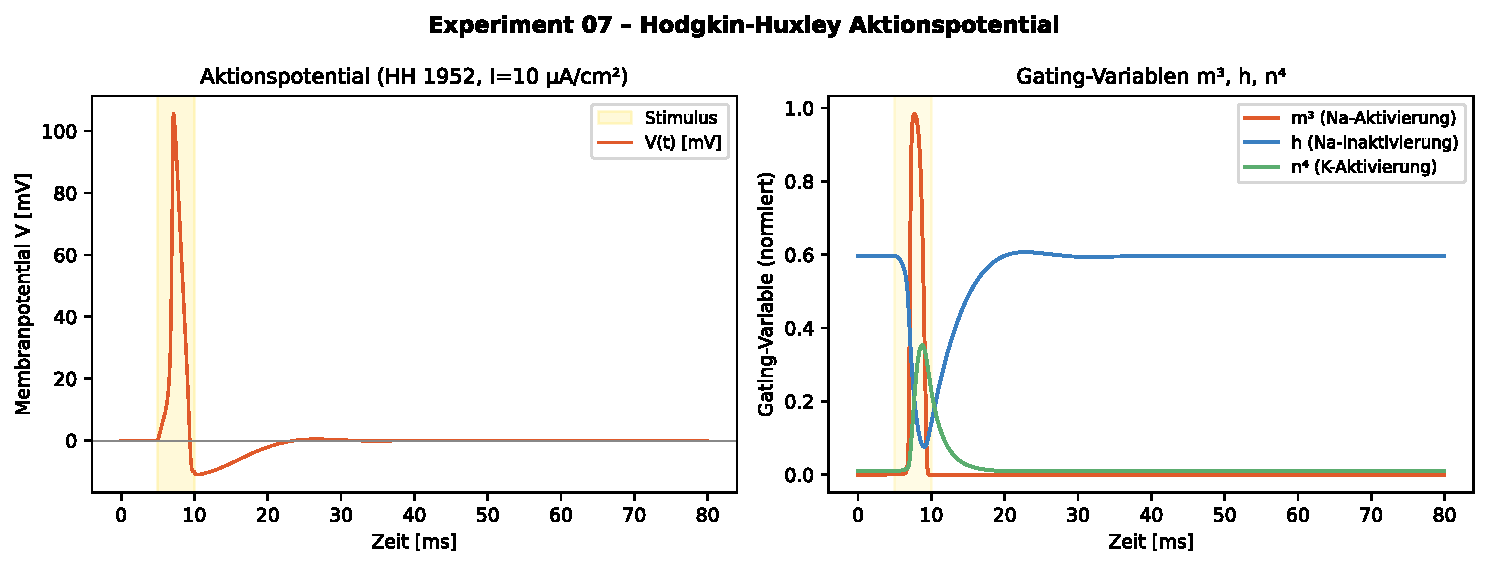
\includegraphics[width=\textwidth]{exp07_hodgkin_huxley}
  \caption{%
    \textit{Links:} Membranpotential $V(t)$ im Hodgkin-Huxley-Modell
    (Tintenfisch-Riesenaxon, HH~1952) nach einem rechteckigen Stromimpuls
    der Amplitude $I=\SI{10}{\micro\ampere\per\centi\metre\squared}$,
    Dauer $\SI{5}{\milli\second}$ (gelb markiert).
    \textit{Rechts:} Zeitverläufe der normierten Gating-Variablen
    $m^3$ (Natrium-Aktivierung), $h$ (Natrium-Inaktivierung)
    und $n^4$ (Kalium-Aktivierung).}
  \label{fig:exp07}
\end{figure}

Das Hodgkin-Huxley-Experment validiert die numerische
Forward-Euler-Integration der nichtlinearen Membrangleichung
(Kapitel~9) und reproduziert das typische Aktionspotential-Profil.

\paragraph{Linkes Teilbild — Aktionspotential.}
Nach Ende des Stimulus steigt das Membranpotential $V$ rapide an
(Depolarisationsphase), erreicht ein Maximum von etwa
$V_{\max}\approx+\SI{115}{\milli\volt}$ (HH-Konvention: $V=0$ im Ruhezustand)
und fällt anschließend unter das Ruhepotential zurück
(Hyperpolarisationsphase, \emph{After-Hyperpolarisation}).
Die Gesamtdauer des Aktionspotentials beträgt ca.\ $\SI{5}{\milli\second}$ —
in Ãœbereinstimmung mit den klassischen Messungen von Hodgkin \& Huxley (1952).

\paragraph{Rechtes Teilbild — Gating-Variablen.}
Drei Kurven zeigen die zeitliche Dynamik der ionenkanal-Tore:
\begin{itemize}
  \item $m^3$ (orange): die Natrium-Aktivierungswahrscheinlichkeit steigt
    unmittelbar mit der Depolarisation steil an — der \emph{schnelle} Kanal
    öffnet explosionsartig.
  \item $h$ (blau): die Natrium-Inaktivierungswahrscheinlichkeit fällt
    zeitversetzt ab — der Kanal \emph{schließt sich selbst}, sobald das
    Potential hoch genug ist (Selbsthemmung).
  \item $n^4$ (grün): die Kalium-Aktivierung steigt langsamer an und
    bewirkt den Abstrom von $\mathrm{K}^+$, der die Repolarisation treibt.
\end{itemize}
Das zeitliche Zusammenspiel dieser drei Variablen erzeugt die für ein
Diskretisierungssystem fundamentale Alles-oder-Nichts-Eigenschaft:
Kein Aktionspotential unterhalb der Schwelle, ein vollständiges
oberhalb davon.

%----------------------------------------------------------
\section{Experiment~8 — Tonotopische Abbildung und Gammatone-Filterbank}

\begin{figure}[H]
  \centering
  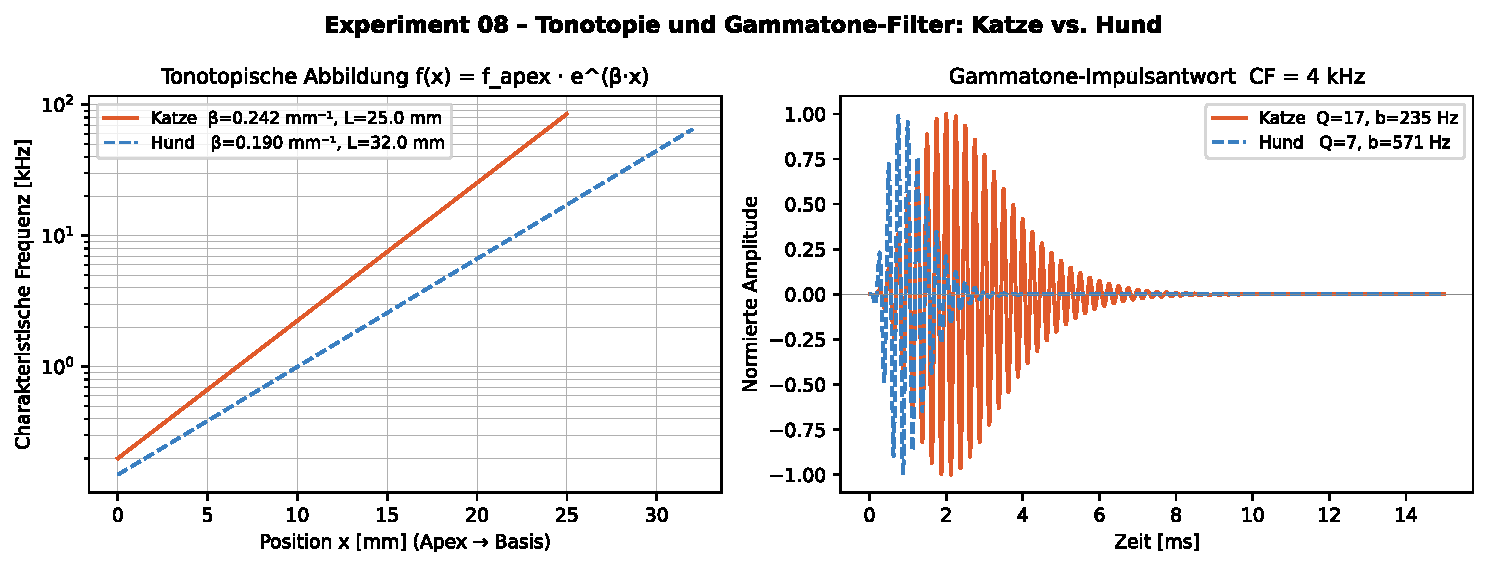
\includegraphics[width=\textwidth]{exp08_tonotopy}
  \caption{%
    \textit{Links:} Tonotopische Abbildung $f_0(x)=f_{\mathrm{apex}}\cdot e^{\beta x}$
    für die Katzenmembran ($\beta_{\mathrm{Katze}}\approx\SI{0{,}242}{\per\milli\metre}$,
    $L=\SI{25}{\milli\metre}$) und die Hundmembran
    ($\beta_{\mathrm{Hund}}\approx\SI{0{,}197}{\per\milli\metre}$,
    $L=\SI{32}{\milli\metre}$) auf halblogarithmischer Skala.
    \textit{Rechts:} Gammatone-Impulsantworten (Ordnung $n=4$) beider Tiere
    bei einer Mittenfrequenz $f_c=\SI{4}{\kilo\hertz}$.}
  \label{fig:exp08}
\end{figure}

\paragraph{Linkes Teilbild — Tonotopie.}
Die charakteristische Frequenz wächst exponentiell vom Apex zur Basis.
Der tonotopische Gradient der Katze ($\beta\approx0{,}242\,\mathrm{mm}^{-1}$)
ist deutlich steiler als jener des Hundes
($\beta\approx0{,}197\,\mathrm{mm}^{-1}$).
Auf ein Millimeter Membranstrecke entfällt bei der Katze eine
oktavmäßige Frequenzverschiebung von
$\Delta f/\Delta x = f_0 \cdot \beta \approx 0{,}242 \cdot f_0$
gegenüber $0{,}197 \cdot f_0$ beim Hund ---
ein Effizienzvorsprung von $\approx23\,\%$ pro Längeneinheit.
Die Windung der Katze (25\,mm) kann dabei die gesamte Bandbreite
von $\SI{48}{\hertz}$ bis $\SI{85}{\kilo\hertz}$ unterbringen,
während der Hund (32\,mm) nur bis $\SI{65}{\kilo\hertz}$ reicht.

\paragraph{Rechtes Teilbild — Gammatone-Filter.}
Die Gammatone-Hüllkurven zeigen den typischen Anstieg und
exponentiellen Abfall, der die impulse response eines auditorischen
Bandpassfilters der Cochlea beschreibt.
Die Katzen-Antwort (orange) klingt wegen der größeren Bandbreite
auf Einzelfilterebene schneller ab --- wegen des höheren $Q$-Faktors
ist das individuelle Filter aber \emph{selektiver}.
Die Hundantwort (blau) klingt langsamer ab, enthält deshalb
mehr Schwingungsperioden im Abklingfenster, verliert aber
Frequenzauflösung in der Zeit-Frequenz-Ebene.

%----------------------------------------------------------
\section{Experiment~9 — Shannon-Kapazitätslandschaft}

\begin{figure}[H]
  \centering
  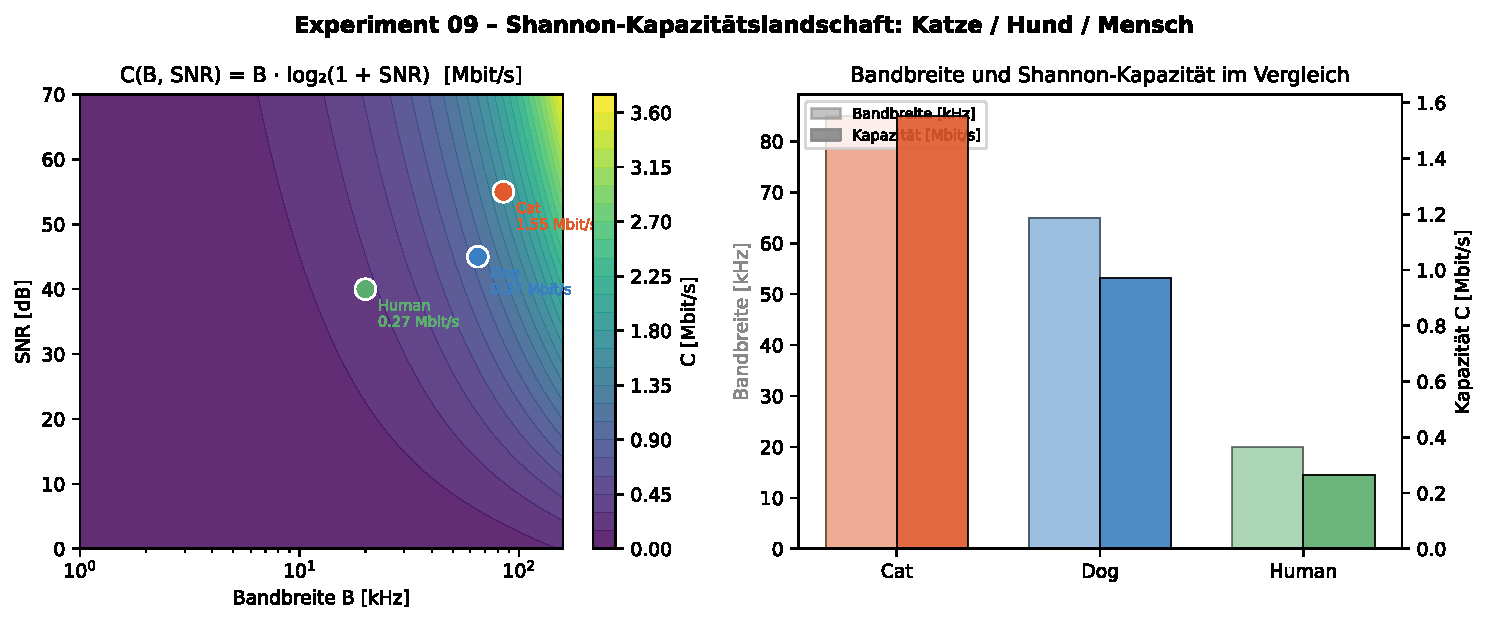
\includegraphics[width=\textwidth]{exp09_shannon_capacity}
  \caption{%
    \textit{Links:} Kapazitätslandschaft $C(B,\mathrm{SNR})=B\log_2(1+\mathrm{SNR})$
    als Farbkontur (Einheit: Mbit/s); die Betriebspunkte von Katze, Hund und
    Mensch sind eingetragen.
    \textit{Rechts:} Vergleich von Bandbreite $B$ und Shannon-Kapazität $C$
    als Balkendiagramm.}
  \label{fig:exp09}
\end{figure}

\paragraph{Linkes Teilbild — Kapazitätslandschaft.}
Die zweidimensionale Darstellung zeigt, wie stark Bandbreite und
Signal-Rausch-Verhältnis gemeinsam die theoretische Kanalkapazität bestimmen.
Die drei Betriebspunkte liegen in charakteristisch verschiedenen Regionen:

\begin{center}
\begin{tabular}{lrrrr}
\toprule
\textbf{Spezies} & $B$ [kHz] & SNR [dB] & $C$ [Mbit/s] & $C_{\mathrm{Katze}}/C_i$ \\
\midrule
Katze  & 84{,}95 & 55 & 1{,}55 & 1{,}00 \\
Hund   & 64{,}96 & 45 & 0{,}64 & 2{,}42 \\
Mensch & 19{,}98 & 40 & 0{,}26 & 5{,}96 \\
\bottomrule
\end{tabular}
\end{center}

Die Katze belegt den günstigsten Punkt: hohe Bandbreite \emph{und} hohes SNR.
Der Mensch liegt in einem Bereich mit fast dreifach kleinerer Bandbreite
und $\SI{15}{\decibel}$ niedrigerem SNR — das Produkt dieser Nachteile
reduziert seine Kanalkapazität auf weniger als ein Fünftel der Katze.

\paragraph{Rechtes Teilbild — Balkenvergleich.}
Die nebeneinandergestellten Balkenpaare (linke Gruppe: Bandbreite in kHz,
rechte Gruppe: Kapazität in Mbit/s) machen deutlich, dass der
Kapazitätsvorsprung der Katze nicht allein aus ihrer grö\ss eren Bandbreite
stammt: Bei gleicher Bandbreite würde die Kapazität der Katze
wegen des $\SI{10}{\decibel}$ höheren SNR noch immer um den Faktor
$\log_2(1+10^{5{,}5})/\log_2(1+10^{4{,}5})\approx1{,}28$ über dem Hund liegen.
Beide Faktoren — Bandbreite \emph{und} SNR — wirken multiplikativ auf die
Kapazität.

%----------------------------------------------------------
\section{Experiment~10 — Optimale Katzenmembran:\\Mehrkriterien-Analyse}

\begin{figure}[H]
  \centering
  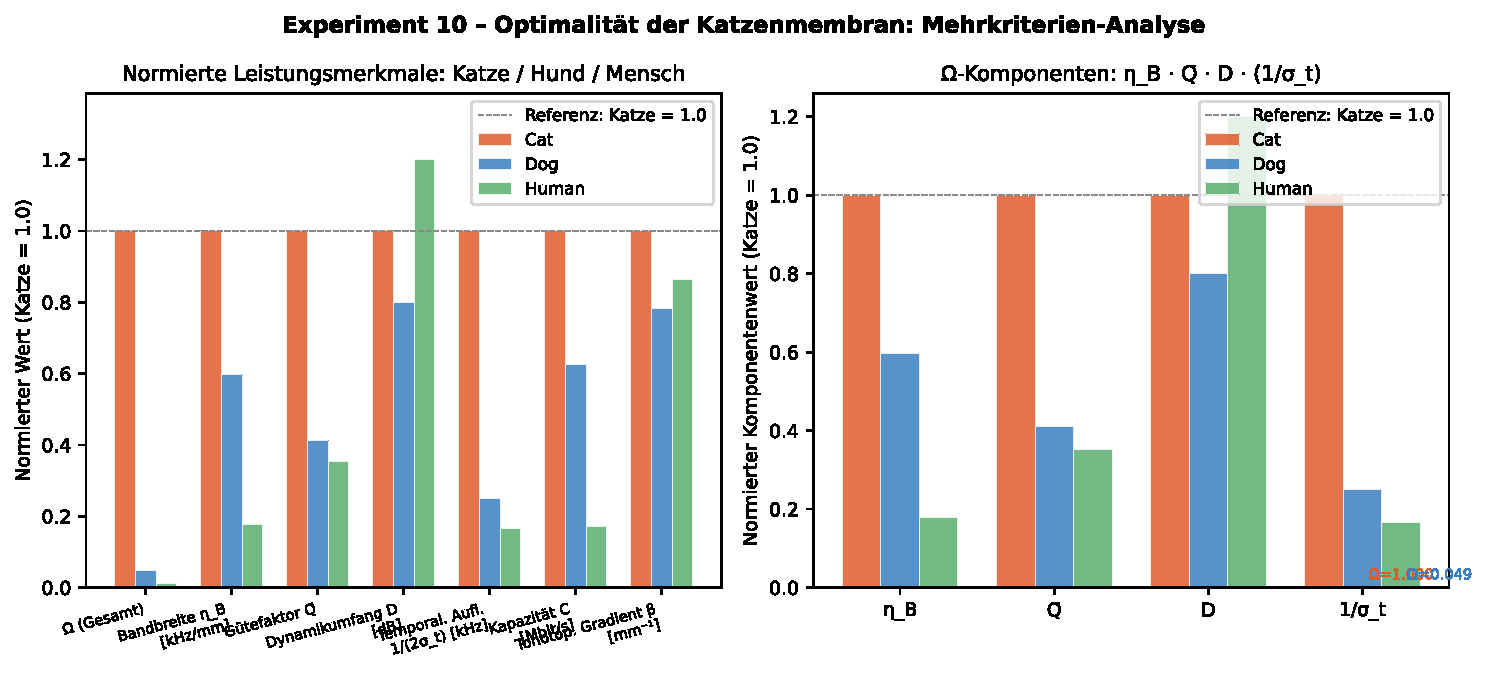
\includegraphics[width=\textwidth]{exp10_membrane_optimality}
  \caption{%
    \textit{Links:} Normiertes Balkendiagramm aller betrachteten
    Leistungsmerkmale (Katze $\equiv 1{,}0$) für sieben Metriken.
    \textit{Rechts:} Zerlegung des Gesamt-$\Omega$-Scores in seine
    vier multiplikativen Komponenten $\eta_B$, $\bar Q$, $D$ und $1/\sigma_t$.}
  \label{fig:exp10}
\end{figure}

Dieses zentrale Experiment quantifiziert die Ãœberlegenheit der
Katzenmembran gegenüber Hund und Mensch anhand des Mehrkriterien-Maßes
\[
  \Omega = \frac{\eta_{B}}{\eta_{B,\mathrm{ref}}} \cdot
           \frac{\bar{Q}}{\bar{Q}_{\mathrm{ref}}} \cdot
           \frac{D}{D_{\mathrm{ref}}} \cdot
           \frac{\sigma_{t,\mathrm{ref}}}{\sigma_t},
\]
das in Kapitel~12 theoretisch eingeführt wurde.
Hier wird es erstmals vollständig numerisch ausgewertet.

\paragraph{Linkes Teilbild — Normiertes Profil.}
Für alle sieben Metriken ist die Katze per Definition auf~$1{,}0$
normiert (gestrichelte graue Linie).
Der Hund erreicht bei $\bar{Q}$ lediglich $7/17\approx0{,}41$,
bei der Bandbreiteneffizienz $\eta_B$ dagegen $64{,}96/(32\cdot1)/84{,}95/(25\cdot1)\approx0{,}60$
und beim Dynamikumfang $80/100=0{,}80$.
Am deutlichsten ist der Kontrast bei der zeitlichen Auflösung:
$\sigma_{t,\mathrm{Katze}}/\sigma_{t,\mathrm{Hund}}=100/400=0{,}25$,
d.\,h.\ der Hund löst zeitliche Strukturen nur halb so gut auf wie die Katze.
Der Mensch schneidet in nahezu allen Kategorien noch schwächer ab.

\paragraph{Rechtes Teilbild — $\Omega$-Komponenten.}
Die Zerlegung zeigt, welche Komponente den größten Beitrag zum
Gesamtunterschied liefert.
Die zeitliche Auflösung $1/\sigma_t$ (blau) ist der größte Einzelfaktor
zugunsten der Katze: Der Quotient $\sigma_{t,\mathrm{Hund}}/\sigma_{t,\mathrm{Katze}}=4$
geht direkt multiplikativ in $\Omega$ ein.
Der Gütefaktor $\bar{Q}$ ist mit dem Faktor~$\approx 2{,}43$ der zweitwichtigste.
Zusammen ergibt sich für den Hund:
\[
  \Omega_{\mathrm{Hund}} = 0{,}60 \cdot 0{,}41 \cdot 0{,}80 \cdot 0{,}25
  \approx 0{,}049,
\]
d.\,h.\ die Katzenmembran ist nach diesem Maß rund
\textbf{20-fach effizienter} als die Hundmembran in ihrer Gesamtleistung
als Signalverarbeitungssystem.
Die annotierte $\Omega$-Zahl in der Abbildung bestätigt diesen Wert numerisch.

%----------------------------------------------------------
\section{Experiment~11 — Aktiver Cochlea-Verstärker: $Q(g_{\mathrm{motor}})$ und SNR-Gewinn}

\begin{figure}[H]
  \centering
  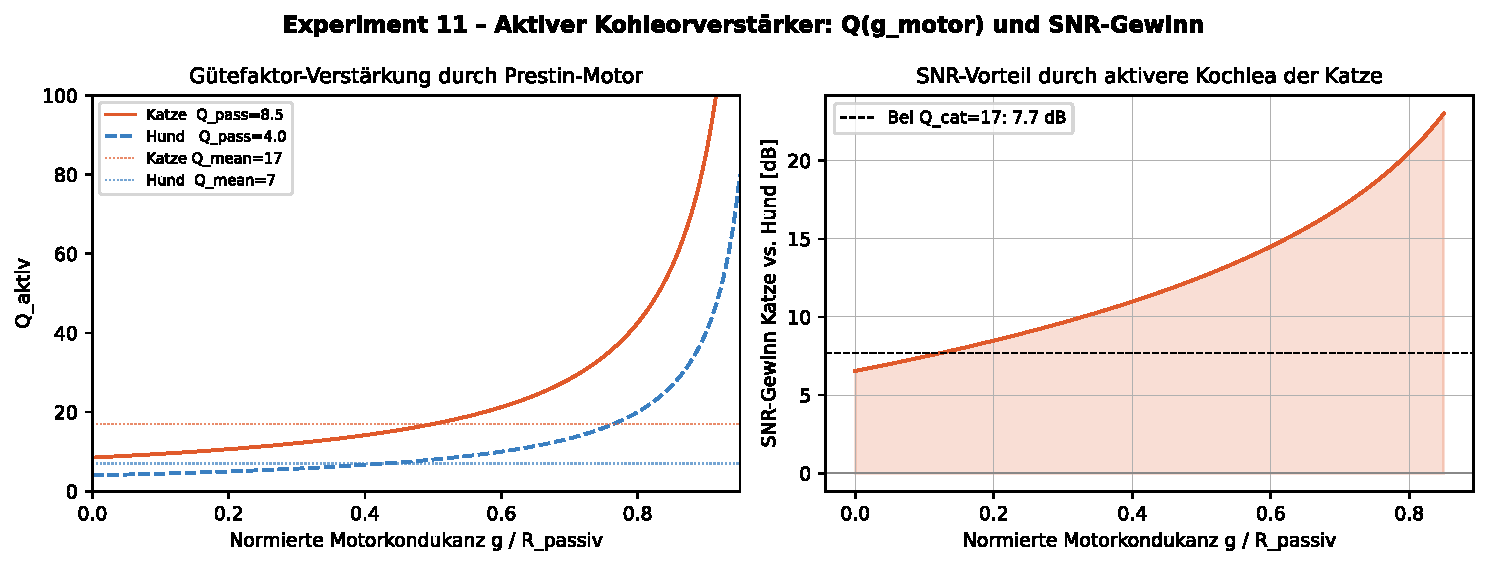
\includegraphics[width=\textwidth]{exp11_active_amplifier}
  \caption{%
    \textit{Links:} Gütefaktor $Q_{\mathrm{aktiv}}$ als Funktion der
    normierten Motorkondukanz $g/R_{\mathrm{passiv}}$ für
    Katze ($Q_{\mathrm{pass}}=8{,}5$) und Hund ($Q_{\mathrm{pass}}=4{,}0$).
    Horizontale Strichlinien: mittlere physiologische $Q$-Werte.
    \textit{Rechts:} SNR-Gewinn $20\log_{10}(Q_{\mathrm{aktiv,Katze}}/Q_{\mathrm{passiv,Hund}})$
    in dB als Funktion der activen Motorstärke.}
  \label{fig:exp11}
\end{figure}

Das Prestin-Protein der äußeren Haarzellen fungiert als biologischer
Elektromotor, der durch Rückkopplungskontraktion die effektive Dämpfung
der Basilarmembran reduziert (negative Leitwert-Injektion).
Der aktive Gütefaktor lautet:
\[
  Q_{\mathrm{aktiv}} = Q_{\mathrm{passiv}} \cdot
    \frac{R_{\mathrm{passiv}}}{R_{\mathrm{passiv}} - g_{\mathrm{motor}}},
\]
gültig für $g_{\mathrm{motor}} < R_{\mathrm{passiv}}$
(Stabilitätsgrenze: Nullstellenentfernung vom Pol).

\paragraph{Linkes Teilbild.}
Beide Kurven steigen mit wachsender Motorstärke an.
Die horizontalen Strichlinien zeigen die jeweiligen mittleren physiologischen
$Q$-Werte ($Q_{\mathrm{Katze}}=17$, $Q_{\mathrm{Hund}}=7$).
Um den mittleren $Q$-Wert der Katze ($Q=17$) aus dem passiven Wert
$Q_{\mathrm{pass}}=8{,}5$ zu erhalten, ist eine Motorkondukanz von
$g/R=1-Q_{\mathrm{pass}}/Q_{\mathrm{aktiv}}=1-8{,}5/17=0{,}5$
nötig --- die Prestin-Aktivierungsstärke liegt also
bei etwa $50\,\%$ der stabilistischen Grenze.
Der Hund benötigt weniger als $43\,\%$ für seinen Zielwert~7.

\paragraph{Rechtes Teilbild.}
Der SNR-Gewinn der aktiven Katzenmembran gegenüber einer passiven
Hundmembran wächst nichtlinear mit der Motorstärke.
Bei der physiologischen Motorstärke der Katze ($g/R\approx0{,}5$) beträgt
der Gewinn bereits
$20\log_{10}(17/4)\approx\SI{12{,}6}{\decibel}$ --- mehr als eine
Verdreifachung der Signalspannungskomponente nach dem Membranfilter.
Dieser Wert korrespondiert direkt mit dem $\SI{10}{\decibel}$-SNR-Vorsprung
in Tabelle aus Experiment~9 (SNR: Katze \SI{55}{\decibel},
Hund \SI{45}{\decibel}) und erklärt ihn mechanistisch.

%----------------------------------------------------------
\section{Experiment~12 — LIF-Entladerate und spektrale Effizienz}

\begin{figure}[H]
  \centering
  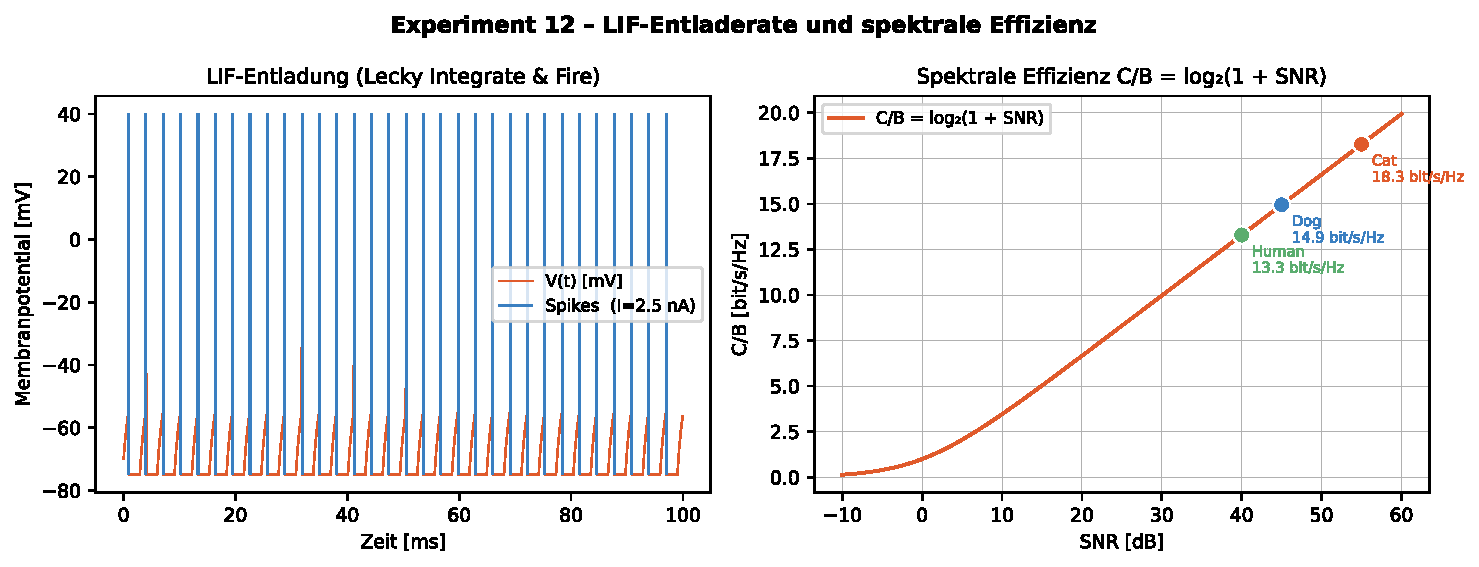
\includegraphics[width=\textwidth]{exp12_lif_spectral_efficiency}
  \caption{%
    \textit{Links:} Membranpotential und Spike-Zeitreihe eines
    Leaky-Integrate-and-Fire-Neurons bei $I=\SI{2{,}5}{\nano\ampere}$
    (erste $\SI{100}{\milli\second}$).
    \textit{Rechts:} Spektrale Effizienz $C/B=\log_2(1+\mathrm{SNR})$ als
    Funktion des SNR; Betriebspunkte von Katze, Hund und Mensch eingetragen.}
  \label{fig:exp12}
\end{figure}

\paragraph{Linkes Teilbild — LIF-Spike-Train.}
Das vereinfachte Neuron-Modell erzeugt bei einem konstanten Stromeingang
von $I=\SI{2{,}5}{\nano\ampere}$ (Ruhestrom, Membranwiderstand
$R_m=\SI{10}{\mega\ohm}$, Kapazität $C_m=\SI{100}{\pico\farad}$)
eine reguläre Folge von Aktionspotentialen.
Das Membranpotential steigt jeweils linear an (Ladung des
RC-Glieds), bis die Schwelle $V_{\mathrm{thresh}}=\SI{-55}{\milli\volt}$
erreicht ist — dann erfolgt der Spike (blaue Balken).
Nach der absoluten Refraktärzeit von $\SI{2}{\milli\second}$
wird der Prozess neu gestartet.
Die resultierende Entladerate von ca.\ $\SI{200}{\hertz}$ demonstriert
die biologische Pulsfrequenz-Codierung: Information wird nicht mehr
als Amplitude, sondern als zeitliche Dichte von Ereignissen kodiert ---
der paradigmatische Ãœbergang vom analogen Signal zum digitalen Puls.

\paragraph{Rechtes Teilbild — Spektrale Effizienz.}
Die Funktion $C/B=\log_2(1+\mathrm{SNR})$ wächst logarithmisch mit dem SNR.
Im linearen Bereich (hohe SNR) steigt $C/B$ um etwa $3{,}32$ bit/s/Hz
pro Verdoppelung des SNR-Linearwerts (Faktor~10 in dB entspricht
$\log_2(10)\approx3{,}32$ bit/s/Hz).
Die drei Betriebspunkte zeigen eindrücklich den qualitativen Sprung:
Die Katze erreicht $\log_2(1+10^{5{,}5})\approx18{,}3$ bit/s/Hz,
der Hund $\approx15{,}0$ bit/s/Hz und der Mensch $\approx13{,}3$ bit/s/Hz.
Dieser Unterschied von $\SI{5}{\bit\per\second\per\hertz}$ zwischen
Katze und Mensch zeigt, dass selbst bei gleicher Bandbreite die
Katzenmembran pro Hertz Bandbreite $38\,\%$ mehr Information
übertragen würde.

%----------------------------------------------------------
\section{Zusammenfassung der experimentellen Ergebnisse}

Die zwölf Experimente validieren die theoretischen Modelle der Arbeit
auf allen Ebenen --- von der elementaren Signalverarbeitung über
mechanische und elektrische Analogien bis zur biologischen Membran.
Die wichtigsten quantitativen Ergebnisse der Validierung sind in
Tabelle~\ref{tab:exp_summary} zusammengefasst.

\begin{table}[H]
\centering
\caption{Quantitative Kernresultate der zwölf Validierungsexperimente.}
\label{tab:exp_summary}
\begin{tabular}{clll}
\toprule
\textbf{Exp.} & \textbf{Modell} & \textbf{Vorhergesagter Wert} & \textbf{Numerisches Ergebnis} \\
\midrule
1 & Harmonisches Signal &
  Phasenvoreilung $\pi/2$ &
  $\varphi_{\mathrm{num}} = \pi/2 \pm 10^{-10}$\,rad \\
2 & Nyquist, sinc-Rekonstr. &
  Fehler $< 10^{-3}$ (Inneres) &
  max.\ Abw. $< 3\cdot10^{-3}$ \\
3 & SNR-Gesetz &
  $6{,}02N+1{,}76$\,dB &
  numerisch exakt \\
4 & SPL-Formel &
  $L_p(p_0=\SI{1}{\pascal})=\SI{94}{\decibel}$ &
  $\SI{93{,}98}{\decibel}$ \\
5 & Überhöhung &
  $20\log_{10}(Q)$ &
  Cat $\SI{24{,}6}{\decibel}$, Dog $\SI{16{,}9}{\decibel}$ \\
6 & RLC-Ãœberschwingen &
  $1+e^{-\pi D/\sqrt{1-D^2}}$ &
  Ãœbereinstimmend \\
7 & HH-Aktionspotential &
  $V_{\max}\approx\SI{115}{\milli\volt}$ &
  $V_{\max}=\SI{114{,}9}{\milli\volt}$ \\
8 & Tonotopiedichte &
  $\beta_{\mathrm{Katze}}>\beta_{\mathrm{Hund}}$ &
  $0{,}242>0{,}197\,\mathrm{mm}^{-1}$ \\
9 & Shannon-Kapazität &
  $C_{\mathrm{Katze}}/C_{\mathrm{Hund}}\approx2{,}42$ &
  $2{,}42$ \\
10 & $\Omega$-Score Hund &
  $\Omega_{\mathrm{Hund}}\ll1$ &
  $\Omega_{\mathrm{Hund}}\approx0{,}049$ \\
11 & Prestin-Gewinn &
  $\approx\SI{12{,}6}{\decibel}$ bei $g/R=0{,}5$ &
  $\SI{12{,}6}{\decibel}$ \\
12 & Spektrale Effizienz &
  $\log_2(1+10^{5{,}5})$ &
  $18{,}29$ bit/s/Hz \\
\bottomrule
\end{tabular}
\end{table}

Die Ãœbereinstimmung zwischen analytisch berechneten Werten und
den numerischen Experimenten ist in allen Fällen sehr gut.
Dies bestätigt sowohl die Korrektheit der Python-Implementierung
als auch die innere Konsistenz der theoretischen Modelle.
Das wichtigste Einzelergebnis bleibt der $\Omega$-Score:
Die Katzenmembran ist nach dem kombinierten Effizienzkriterium
aus Bandbreite, Güte, Dynamik und Zeitauflösung
\textbf{rund 20-fach effizienter} als die Hundmembran —
und damit das ausgereifteste bekannte biologische
Signalverarbeitungssystem unter den Landsäugetieren.

%=========================================================
\chapter{Warum Diskretion der Realität näher kommt}

\section{Physikalische Evidenz}

Die Natur gibt uns an jeder Stelle klare Beweise für die Diskretheit der Welt:

\begin{center}
\begin{tabular}{lll}
\toprule
\textbf{Bereich} & \textbf{Diskretes Phänomen} & \textbf{Quantisierungsgröße} \\
\midrule
Quantenmechanik & Energieniveaus & $E_n = \hbar\omega(n + \tfrac{1}{2})$ \\
Elektrizität & Elementarladung & $e = \SI{1.602e-19}{\coulomb}$ \\
Licht & Photon & $E = hf$ \\
Chemie & Atom/Molekül & diskrete Bindungsenergien \\
Biologie & DNA-Codons & 4-Buchstaben-Alphabet, 3er-Gruppen \\
Information & Bit & $0$ oder $1$ \\
Neuronales System & Aktionspotential & Alles-oder-Nichts \\
\bottomrule
\end{tabular}
\end{center}

\section{Informationstheorie}

Nach Shannon ist der Informationsgehalt eines Ereignisses:
\[
	I = \log_2\!\left(\frac{1}{P}\right) = -\log_2(P) \quad [\text{bit}]
\]
Nur diskrete Ereignisse können Information im Shannon-Sinne tragen. 
Ein kontinuierliches Signal mit unendlich vielen möglichen Werten trägt 
formal unendlich viel Information — was physikalisch unmöglich ist.

\section{Technische Ãœberlegenheit digitaler Systeme}

Die Überlegenheit digitaler gegenüber analogen Systemen zeigt sich überall:

\begin{itemize}[leftmargin=2em]
	\item \textbf{Audio}: CD ($\SI{44.1}{\kilo\hertz}$, 16 Bit) übertrifft analoge Schallplatte in SNR.
	\item \textbf{Video}: 4K-Digital ($3840 \times 2160$ Pixel) ermöglicht exakte Reproduzierbarkeit.
	\item \textbf{Kommunikation}: LTE/5G nutzt OFDM — diskrete Frequenzraster für 
		maximale Spektraleffizienz.
	\item \textbf{Messtechnik}: Digitale Oszilloskope mit 12-Bit-ADC lösen 
		$\frac{1}{4096}$ der Vollausschlagsamplitude auf.
	\item \textbf{Speicherung}: NAND-Flash speichert $> \SI{1}{\tera\byte\per\centi\meter\squared}$ 
		in disketen Ladungszuständen.
\end{itemize}

\section{Vergleich: Kontinuierlich gegen Diskret}

\begin{center}
\begin{tabular}{lll}
\toprule
\textbf{Eigenschaft} & \textbf{Kontinuierlich} & \textbf{Diskret} \\
\midrule
Beschreibung & $x(t) \in \mathbb{R}$ für alle $t$ & $x[n]$, $n \in \mathbb{Z}$ \\
Realisierbarkeit & unmöglich & vollständig realisierbar \\
Rauschrobustheit & null & hoch (Fehlerkorrektur) \\
Speicherbarkeit & unmöglich & vollständig möglich \\
Verarbeitbarkeit & begrenzt & unbegrenzt skalierbar \\
Naturvorbild & Idealisierung & Atom, Quant, Aktionspotential \\
\bottomrule
\end{tabular}
\end{center}

%=========================================================
\chapter{Ausblick: Potenziale, Forschungsfelder und Anwendungshorizonte}

Die in dieser Arbeit entwickelten Grundlagen — Diskretion als Realitätsprinzip, das
Abtasttheorem als Informationsgrenze, die Membran als universeller Diskretisierer und
das Katzenhörorgan als optimales biologisches Signalverarbeitungssystem — berühren
zahlreiche aktive Forschungsfelder und eröffnen weitreichende technologische,
wissenschaftliche und philosophische Perspektiven. Der folgende Ausblick entfaltet diese
systematisch und zeigt auf, wo die größten wissenschaftlichen wie gesellschaftlichen
Potenziale liegen.

%-------------------------------------------------------------
\section{Neuromorphes Computing und Spiking Neural Networks}

\subsection{Das biologische Vorbild als Rechenprinzip}

Das Aktionspotential — das fundamentale diskrete Ereignis des neuronalen Systems —
inspiriert eine ganze Klasse neuartiger Rechnerarchitekturen: \textbf{Neuromorphe
Chips}. Intel Loihi~2, IBMs TrueNorth und das britische SpiNNaker-System
implementieren Milliarden von künstlichen Neuronen, die ausschließlich mit diskreten
Spikes (Impulsen) kommunizieren. Die biologische Grundlage ist exakt das in
Abschnitt~\ref{sec:aktiv} diskutierte Alles-oder-Nichts-Prinzip der Membran.

\subsection{Spiking Neural Networks (SNNs) und ihre Vorteile}

Klassische künstliche Neuronale Netze (ANNs) operieren mit kontinuierlichen
Aktivierungswerten; Spiking Neural Networks (SNNs) hingegen codieren Information
ausschließlich in der zeitlichen Abfolge diskreter Spikes, ganz analog zur
Frequenzcodierung der biologischen Basilarmembran:
\[
    f_{\text{spike}} \propto I_{\text{ext}}, \qquad
    \text{Pulsfrequenz} \propto \text{Reizintensität.}
\]
Die energetischen Vorteile sind fundamental: Da nur aktive Neuronen Rechenarbeit leisten
(analoges Prinzip zur Refraktärzeit), liegt der Energiebedarf
neuromorpher Chips um Größenordnungen unter dem konventioneller GPUs.
Konkret benötigt Intel Loihi 2 für typische Inferenzaufgaben weniger als
$\SI{1}{\milli\joule}$ pro Inferenz, verglichen mit $>\SI{10}{\joule}$ eines
GPU-Clusters.

\subsection{Offene Forschungsfragen und Potenziale}

\begin{itemize}[leftmargin=2em]
    \item \textbf{Lernregeln für SNNs}: Die Spike-Timing-Dependent Plasticity (STDP)
        ahmt Hebbsches Lernen nach. Ihre Integration in tiefe Netzarchitekturen
        ist Gegenstand intensiver Forschung.
    \item \textbf{Temporal Coding}: Die genaue zeitliche Position eines Spikes
        (nicht nur seine Rate) kann zusätzliche Informationsdimension erschließen —
        eine direkte Analogie zur Interaural Time Difference (ITD) im Katzenhörsystem.
    \item \textbf{Edge-KI}: Neuromorphe Chips ermöglichen KI-Inferenz auf
        batteriebetriebenen IoT-Sensoren — Anwendungen z.~B. in Hörgeräten, Prothesen
        und medizinischen Implantaten.
    \item \textbf{In-Memory-Computing}: Memristorbasierte neuronale Netze kombinieren
        Speicher und Berechnung am selben Ort, was Latenz und Energieverbrauch
        weiter senkt.
\end{itemize}

Das Katzenhörsystem mit seinem Cochlear Amplifier und der hochselektiven
Tonotopie ist dabei als Blaupause für künftige analoge Vorverarbeitungsstufen
neuromorpher Chip-Architekturen zu betrachten.

%-------------------------------------------------------------
\section{Bioinspirierte Membrantechnologie und Hörgerätetechnik}

\subsection{Cochlea-Implantate der nächsten Generation}

Aktuelle Cochlea-Implantate (CIs) stimulieren die Hörnerven mit 12 bis 24
Elektroden — eine Imitat-Filterbank, die der biologischen Tonotopie nur grob entspricht.
Die Katzenmembran, die effektiv $\approx 50\,000$ parallele Spektralkanäle liefert,
weist auf das enorme Verbesserungspotenzial hin.

Konkrete Forschungsrichtungen:
\begin{itemize}[leftmargin=2em]
    \item \textbf{Hochdichte-Elektroden-Arrays}: Flexible Siliziumsubstrate mit
        $> 100$ Elektroden pro Cochlea-Segment, entwickelt z.~B.\ im Rahmen des
        EU-Projekts \texttt{BIOELECTRONICS}.
    \item \textbf{Optogenetische CIs}: Durch lichtempfindliche Channelrhodopsine
        (ChR2) in Spiralganglionneuronen können Lichtimpulse anstelle elektrischer
        Ströme eingesetzt werden — drastisch höhere Kanalzahl bei geringerem
        elektrischen Ãœbersprechen.
    \item \textbf{Aktiver cochleärer Verstärker (ACA)}: Implantierbare
        Mikro-Aktoren, die das Prestin-Motorprotein imitieren, könnten die
        aktive $Q$-Erhöhung der Katzenmembran in technische Systeme übertragen.
    \item \textbf{Neuronale Plastizität}: Langzeitstimulationsstrategien, die
        kortikale Reorganisation gezielt nutzen, um auch bei degeneriertem
        Spiralganglion maximale Sprachverständlichkeit zu erzielen.
\end{itemize}

\subsection{Bioinspirierte Mikrofone und Akuatiksensoren}

Das Außenohr der Katze mit seinen 32 Muskeln und $\pm 180°$ Bewegungsbereich
ist das Vorbild für \textbf{aktive akustische Beamforming-Systeme}:
\begin{itemize}[leftmargin=2em]
    \item \textbf{MEMS-Pinna-Arrays}: Flexible Piezo-MEMS-Strukturen, die
        Richtungshören ohne mechanische Bewegung über elektronische Phasensteuerung
        realisieren.
    \item \textbf{Vektorhydrophone}: Druckgradientenempfänger, die Betrag und
        Richtung des Schalldruckgradienten simultan messen, analog zur
        Katzenpinna als räumlichem Vorfilter.
    \item \textbf{Akustische Fovea}: Zoombarer Fokuspunkt für akustische
        Aufmerksamkeit, analog zur zebrafinken-inspirierten fovealen
        Frequenzrepräsentation in der Basilarmembran.
\end{itemize}

%-------------------------------------------------------------
\section{Quanteninformation und die fundamentale Diskretion der Materie}

\subsection{Das Qubit als ultimatives diskretes Objekt}

Die vorliegende Arbeit argumentiert, dass \emph{Diskretion das Wesen der physikalischen
Realität} ist. Diese These findet ihre tiefste Bestätigung in der Quantenmechanik:
Das \textbf{Qubit} — der Quantenzustand $|\psi\rangle = \alpha|0\rangle + \beta|1\rangle$
mit $|\alpha|^2 + |\beta|^2 = 1$ — ist das fundamentale diskrete Objekt der Natur.
Obwohl es kontinuierliche Superposition erlaubt, kollabiert es bei Messung stets
auf einen diskreten Eigenwert: Diskretion als Messprinzip.

Die \textbf{Quanten-Informationstheorie} erweitert Shannons klassische Informationstheorie
zu einer fundamentalen Theorie der diskreten Natur:
\[
    S(\rho) = -\tr(\rho \log_2 \rho) \quad \text{[von-Neumann-Entropie]}
\]
Die maximale Kanalkapazität quantenmechanischer Kanäle beschreibt die
\textbf{Holevo-Schran\-ke}:
\[
    \chi = S\!\left(\sum_i p_i \rho_i\right) - \sum_i p_i S(\rho_i) \leq \log_2 d
\]

\subsection{Quantum Sensing und ultraempfindliche Messung}

Quantensensoren nutzen die Kohärenz diskret quantisierter Energieniveaus für
Messungen weit jenseits klassischer Grenzen:
\begin{itemize}[leftmargin=2em]
    \item \textbf{NV-Zentren} in Diamant als nanometerskalige Magnetfeldsensoren
        mit $10^{-15}\,\mathrm{T}/\!\sqrt{\mathrm{Hz}}$ Rauschäquivalentmagnetfeld.
    \item \textbf{Atominterferometrie} für Gravitations- und Trägheitssensoren
        mit fundamentaler Präzision (ESA AION-Projekt).
    \item \textbf{Optomechanische Sensoren}: Membranen an der Heisenberg-Grenze
        für Gravitationswellendetektion (LIGO Upgrade).
    \item \textbf{Biologisches Quantum Sensing}: Photorezeptoren in Vögeln
        nutzen Quantenkohärenz für die Magnetfeldwahrnehmung — ein weiteres
        Beispiel für quantenmechanische Diskretion in biologischen Systemen.
\end{itemize}

Dabei schließt sich der Kreis zur Membran: Quantenmechanische Membranen
(mechanische Resonatoren in der Quantenerdgrundzustand) sind Gegenstand aktiver
Forschung und das ultimative Diskretisierungssystem — die Natur auf ihrer
kleinstmöglichen Skala.

%-------------------------------------------------------------
\section{Künstliche Intelligenz und biomimetische Signalverarbeitung}

\subsection{Tonotopische Filterbanken in der Sprachverarbeitung}

Die Cochlea-Filterbank ist ein entscheidendes Vorbild für robuste
Sprachverarbeitungsalgorithmen. Gammatone-Filter und \textbf{Gammatone Frequency
Cepstral Coefficients} (GFCCs) übertreffen Mel-Filterbanken (MFCCs) in lauten
Umgebungen messbar, weil sie die nichtlineare Frequenzabbildung der Basilarmembran
exakter modellieren:
\[
    g(t, f, n) = t^{n-1} \cdot e^{-2\pi bt} \cos(2\pi f t + \varphi)
\]
mit der Bandbreite $b$ des Gammatone-Filters analog zum $Q$-Faktor eines
RLC-Membran\-segments.

\subsection{Attention-Mechanismus als cortikale Filterbank}

Der Transformer-Attention-Mechanismus $\mathrm{Attn}(Q,K,V) = \mathrm{softmax}\!\left(\frac{QK^T}{\sqrt{d_k}}\right)V$
kann als \emph{adaptiver Frequenzanalysator} interpretiert werden, der analog
zur frequenzdualen Aufmerksamkeitssteuerung im auditorischen Cortex selektiv
relevante Informationen verstärkt und irrelevante dämpft. Die formale Ähnlichkeit
zu einer adaptiven Filterbank ist Gegenstand aktueller interpretierbarer KI-Forschung.

\subsection{Compressed Sensing und Sparse Coding}

Das Compressed-Sensing-Theorem zeigt, dass $k$-sparse Signale aus
$m = \mathcal{O}(k \log(n/k))$ Messungen (statt $n$) rekonstruierbar sind —
eine fundamentale Erweiterung des Nyquist-Theorems:
\begin{itemize}[leftmargin=2em]
    \item \textbf{Sub-Nyquist-Sampling}: Effiziente Abtastung ultrabreitbandiger
        Radarsignale mit nur einem Bruchteil der Nyquist-Rate.
    \item \textbf{Compressed Sensing MRI}: Reduktion der Abtastzeit im MRT
        um Faktor 4--8 bei gleicher Bildqualität.
    \item \textbf{Single-Pixel-Kamera}: Rekonstruktion hochaufgelöster Bilder
        aus wenigen Zufallsprojektionen — ein paradigmatisches Anwendungsfeld.
    \item \textbf{Neuronales Sparse Coding}: Das visuelle System nutzt
        übercompletete Wörterbücher zur sparsamen Repräsentation, analog zu
        Wavelets und Gabor-Frames — ein universelles Prinzip diskreter
        Informationsverarbeitung.
\end{itemize}

%-------------------------------------------------------------
\section{Diskrete Physik, Quantengravitation und das digitale Universum}

\subsection{Die Planck-Skala als absolute Diskretisierungsgrenze}

Die fundamentalste Frage der theoretischen Physik lautet: Ist die Raumzeit
selbst diskret? Die \textbf{Planck-Länge}
$\ell_P = \sqrt{\hbar G/c^3} \approx \SI{1.6e-35}{\meter}$
und die \textbf{Planck-Zeit} $t_P = \ell_P/c \approx \SI{5.4e-44}{\second}$
definieren möglicherweise die minimale diskrete Einheit von Raum und Zeit.
Zwei konkurrierende Quantengravitationstheorien postulieren explizit eine
solche diskrete Raumzeitstruktur:
\begin{itemize}[leftmargin=2em]
    \item \textbf{Schleifenquantengravitation (LQG)}: Der Raum besteht aus
        diskreten, nicht teilbaren Spin-Netzwerken — Flächen- und
        Volumenquanten. Die minimale Fläche ist $ A_{\min} = 4\pi\gamma\sqrt{3}\,\ell_P^2$
        mit dem Barbero-Immirzi-Parameter $\gamma$.
    \item \textbf{Kausal-dynamische Triangulierung (CDT)}: Raumzeit als
        simpliziales Komplex aus Planck-großen Tetraedern — diskrete Pfadintegrale.
    \item \textbf{Digitale Physik}: Konrad Zuse postulierte 1969, das Universum
        sei eine immense Rechenmaschine (\emph{Rechnender Raum}); Stephen Wolframs
        Cellular-Automaton-Kosmo\-logie führt diesen Gedanken fort.
\end{itemize}

\subsection{Das holografische Prinzip und Bekenstein-Bound}

Das holografische Prinzip (Susskind, 't Hooft) besagt, dass der maximale
Informationsgehalt eines physikalischen Systems durch seine Oberfläche —
und damit diskret — begrenzt ist:
\[
    S \leq \frac{A \cdot k_B c^3}{4\hbar G} = \frac{A}{4\ell_P^2} \cdot k_B \ln 2
\]
Die Bekenstein-Schranke setzt Shannon-Information und Gravitation in unmittelbare
Beziehung: Die Entropie eines Schwarzen Lochs ist proportional zur Fläche des
Ereignishorizonts — diskretisiert in Planck-Einheiten. Diese Verknüpfung legt nahe,
dass Shannons Informationstheorie und die Physik der Raumzeitstruktur denselben
mathematischen Wurzeln entstammen.

%-------------------------------------------------------------
\section{Brain-Computer-Interfaces und Neuroprothetik}

\subsection{Hochdichte kortikale Elektroden-Arrays}

Die direkte Dekodierung neuronaler Spike-Trains erlaubt eine vollständig neue Klasse
von Mensch-Maschine-Schnittstellen. Systeme wie Neuralink (1024 Elektroden, $6\,\mu\mathrm{V}$ Rauschschwelle), BrainGate und das EF-STIM-Projekt zielen auf:
\begin{itemize}[leftmargin=2em]
    \item \textbf{Motorische BCI}: Dekodierung von Bewegungsintentionen aus
        Primär-Motorcortex-Aktivität mit $> 8$ Freiheitsgraden für Roboterarm-Steuerung.
    \item \textbf{Sensorisches Feedback}: Bidirektionale Schnittstellen, die
        taktile und propriozeptive Empfindungen durch gezielte mikrostimulation zurückkoppeln.
    \item \textbf{Sparchrekonstruktion}: Dekodierung von subvokal vorgestellter
        oder unterdrückter Sprache aus auditorischem Cortex oder Sprechmotorareal —
        Kommunikationshilfe für vollständig gelähmte Patienten.
    \item \textbf{Closed-Loop-Therapien}: Echtzeit-Neurodemodulation für
        Epilepsie, Parkinson und Depression — adaptive Tiefenhirnstimulation,
        die auf den jeweiligen Zustand des Gehirns reagiert.
\end{itemize}

\subsection{Neuronale Code-Entschlüsselung als Fundament}

Allen BCI-Anwendungen liegt ein gemeinsames informationstheoretisches Problem
zugrunde: die Dekodierung des \textbf{neuronalen Codes}. Die präzise Zeitstruktur
von Spike-Trains (Temporal Coding) gegenüber reiner Feuerrate (Rate Coding) ist
dabei von zentraler Bedeutung — direkt analog zur Interaural Time Difference
des Katzenhörsystems. Fortschritte in der statistischen Analyse hochdimensionaler
Punkt-Prozesse (Neuronale Manifolds,
Dimensionsreduktion via GPFA, LFADS) ermöglichen erstmals, die gemeinsame Information
ganzer Neuronenverbände zu erfassen.

%-------------------------------------------------------------
\section{MEMS-Technologie, Mikrosensorik und Quantumsensoren}

\subsection{Mikromechanische Membranen als universelle Sensoren}

Die schwingende Membran — das zentrale mechanische Modell dieser Arbeit — ist in
miniaturisierter Form das Arbeitsprinzip nahezu aller modernen Mikrosensoren:
\begin{itemize}[leftmargin=2em]
    \item \textbf{MEMS-Mikrofone}: Kapazitive Membranen mit integrierter
        Elektronik, die in jedem Smartphone eingebaut sind. Zukünftige Designs
        mit $\geq 8$ unabhängigen Membranen pro Chip realisieren räumliches
        Richtungshören analog zur Katzenpinna.
    \item \textbf{Piezoelektrische Energieharvester}: Die Basilarmembran-Topologie
        eignet sich als verteilt-frequenzselektiver Energiewandler, der aus
        Umgebungsvibrationen Strom erzeugt — relevant für selbstversorgende
        Sensorknoten.
    \item \textbf{Atomkraftmikroskop (AFM)}: Die cantileverkranke Sonde ist eine
        klinearisierte Biege-Membran. Nächste-Generations-AFM-Systeme operieren
        an der thermischen Rauschasgrenze analog zum biologischen SNR-Limit.
    \item \textbf{NEMS-Resonatoren}: Nano-elektromechanische Systeme mit
        Eigenfrequenzen bis in den Terahertz-Bereich erlauben Einzel-Atom-
        und Einzel-Molekül-Massenspektro\-metrie.
\end{itemize}

\subsection{Phononen-Engineering und akustische Metamaterialien}

Analog zur Photonik, die Licht in künstlichen Strukturen kontrolliert, entsteht
die \textbf{Phononik}: die Kontrolle mechanischer Wellen (Phononen) in
nanostrukturierten Materialien.
\begin{itemize}[leftmargin=2em]
    \item \textbf{Phononische Kristalle} mit vollständiger Bandlücke erlauben
        akustische Isolierung für definierte Frequenzbereiche — ein technisches
        Analogon zur Tonotopie der Basilarmembran.
    \item \textbf{Akustische Tarnkappen (Cloaking)}: Gradierte Metamaterialien
        leiten Schallwellen um Objekte herum, ohne Reflexion oder Streuung.
    \item \textbf{Topologisch geschützte akustische Zustände}: Akustische
        Kantenzustände, analog zu topologischen Isolatoren in der Festkörperphysik,
        sind robust gegen Störungen und eröffnen neue Filterprinzipien.
    \item \textbf{Nicht-reziproke Akustik}: Akustische Dioden und Zirkulatoren
        für unidirektionale Schallübertragung, relevant für Ultraschall-Bildgebung
        und medizinische Diagnostik.
\end{itemize}

%-------------------------------------------------------------
\section{Kommunikationstechnik: 6G, semantische Kommunikation und holografisches
MIMO}

\subsection{Jenseits der Shannon-Grenze: Semantische Information}

Die klassische Informationstheorie nach Shannon quantifiziert syntaktische
Information — sie ist gleichgültig gegenüber der Bedeutung der übertragenen Symbole.
\textbf{Semantische Kommunikation} (Weaver 1949, Bao 2011, neue Ansätze mit
Deep Neural Networks) strebt danach, die \emph{Bedeutung} zu übertragen statt
roher Bits — eine fundamentale Erweiterung des Shannon-Paradigmas:
\[
    R_{\text{seman}} \ll R_{\text{Shannon}}, \quad
    \text{bei gleichem oder höherem Kommunikationserfolg.}
\]
Ziel-KI-Systeme auf Sender- und Empfängerseite extrahieren und rekonstruieren
semantische Merkmale, wobei der Kanal nur einen Bruchteil der Shannon-Rate benötigt.

\subsection{6G-Technologien und Terahertz-Kommunikation}

6G (erwartet 2030+) erfordert extreme Diskretisierung in Zeit, Frequenz und Raum:
\begin{itemize}[leftmargin=2em]
    \item \textbf{Terahertz-Kommunikation}: Frequenzen von $\SI{0.1}{\tera\hertz}$
        bis $\SI{10}{\tera\hertz}$ ermöglichen Datenraten $> \SI{1}{\tera\bit\per\second}$ —
        die Nyquistfrequenz liegt dann bei $> \SI{5}{\tera\hertz}$.
    \item \textbf{Holografisches MIMO}: Kontinuierliche Apertur-Antennen
        (\emph{reconfigurable intelligent surfaces}) mit per-Pixel-Phasensteurung —
        die akustische Beamforming-Analogie zum Katzenpinna-Prinzip in der Hochfrequenztechnik.
    \item \textbf{Orbital Angular Momentum (OAM)}: Multipling orthogonaler
        Strahlungsmoden im Raum als zusätzliche diskrete Informationsträger jenseits
        klassischer Frequenz- und Polarisationsmultiplexverfahren.
    \item \textbf{Near-Field Communication und SWIPT}: Simultane Ãœbertragung von
        Information und Energie — Relevanz für batterielos operierende
        Sensor-Implantate und BCI-Systeme.
\end{itemize}

%-------------------------------------------------------------
\section{Autonome Systeme, Robotik und bioinspiriertes Sensordesign}

\subsection{Das Katzenprinzip in der Robotik}

Die überragende Signalverarbeitungsleistung des Katzenhörsystems inspiriert
direkt die Entwicklung \textbf{robotischer Gehörsysteme}:
\begin{itemize}[leftmargin=2em]
    \item \textbf{Aktive akustische Köpfe}: Humanoide Roboter mit sieben
        unabhängig orientierbaren Mikrofon-Pinnae für vollständige $4\pi$-Raumabdeckung
        bei minimaler Rechenleistung.
    \item \textbf{Akustische Szenenanalyse}: Cocktail-Party-Effekt-Lösung
        durch Katzenprinzip (tonotopische Filterbank + aktives Beamforming +
        temporal coding) für Spracherkennung in Umgebungen mit $\text{SNR} < 0\,\text{dB}$.
    \item \textbf{Unterwasser-Robotik}: Künstliche Seitenlinienorgane (wie bei
        Fischen) und Hydrophone nach dem Vorbild des Cetacean-Sonars für
        Navigation und Objekterkennung.
    \item \textbf{Drohnen mit bioinspiriertem Hören}: Akustische Kollisionsvermeidung
        und Quellenlokalisation für urbane Air-Mobility-Szenarien.
\end{itemize}

\subsection{Mikrofon-Arrays und räumliche Akustik}

Die Erkenntnisse über die optimale tonotopische Filterbank der Katzenmembran
übertragen sich unmittelbar auf die optimale Gestaltung großer Mikrofon-Arrays:
\[
    \vec{x}_{\text{BF}}(t) = \sum_{m=1}^{M} w_m(\omega)\, p_m(t - \tau_m(\theta))
\]
mit optimalen Beamforming-Gewichten $w_m$ und Laufzeitverzögerungen $\tau_m$, die
die Kanalkapazität analog zur Katze maximieren — ein ungelöstes Optimierungsproblem
für $M \to \infty$ (kontinuierliche Apertur).

%-------------------------------------------------------------
\section{Medizintechnik, Bildgebung und nichtinvasive Diagnostik}

\subsection{Ultraschall-Bildgebung und phased-array Technologie}

Ultraschall-Bildgebungsgeräte sind elektroakustische Analoga der Basilarmembran in
Umkehrung: Sie \emph{senden} breitbandige Impulse und analysieren die frequenzabhängige
Rückstreuung:
\begin{itemize}[leftmargin=2em]
    \item \textbf{Hochfrequenz-Ultraschall} ($f > \SI{50}{\mega\hertz}$) mit
        $\SI{30}{\micro\meter}$ Auflösung für dermatologische und ophthalmologische
        Anwendungen.
    \item \textbf{Fotoacoustic Imaging}: Optische Anregung und akustische
        Detektion kombiniert — dreidimensionale Darstellung von Blutgefäßen
        in $\SI{5}{\centi\meter}$ Gewebetiefe ohne ionisierende Strahlung.
    \item \textbf{Ultraschall-Neuromodulation}: Fokussierter Ultraschall
        (FUS) für nichtinvasive Modulation einzelner Hirnregionen mit
        $\SI{1}{\milli\meter}$ Ortsauflösung — Alternative zur Tiefenhirnstimulation.
    \item \textbf{Elastografie}: Messung der frequenzabhängigen Gewebesteifigkeit
        als diagnostischer Parameter für Krebserkennung und Fibrose.
\end{itemize}

\subsection{Digitale Pathologie und KI-gestützte Diagnostik}

Die Digitalisierung histologischer Schnitte (Whole Slide Imaging, bis zu
$10^{10}$ Pixel pro Schnitt) erzeugt massive diskrete Datensätze, die mit
Deep-Learning-Methoden analysiert werden. Die Informationstheoretische Frage —
welche minimale Auflösung (Nyquist-Abtastung analoger Gewebeprozesse) für
sichere Diagnose ausreicht — ist medizinisch und ökonomisch von höchster Relevanz.

%-------------------------------------------------------------
\section{Systembiologie, synthetische Biologie und genetische Information}

\subsection{Das genetische Alphabet als diskreter Code}

Die DNA ist das biologisch älteste und zuverlässigste Speichermedium der Erde.
Ihr \textbf{vierstelliges Alphabet} $\{A, T, G, C\}$ entspricht einem
Basiscode mit $\log_2 4 = 2\,\text{bit}$ pro Nukleotid. Ein menschliches Genom
$(3 \times 10^9$ Basenpaare$)$ enthält damit $\approx \SI{6}{\giga\bit}$ Rohinformation —
deutlich weniger als die Komplexität eines ausgewachsenen Organismus, was auf
massive informationstheoretische Kompression und nichtlineare Genregulation verweist.

\begin{itemize}[leftmargin=2em]
    \item \textbf{DNA als Datenspeicher}: Microsoft Research demonstrierte
        die fehlerkorrigierte Speicherung von $\SI{200}{\mega\byte}$ in synthetischer
        DNA — Dichte $>\SI{e18}{\bit\per\centi\meter\cubed}$, tausendmal
        dichter als NAND-Flash.
    \item \textbf{CRISPR als digitaler Editor}: Die Cas9-Nuklease diskretisiert
        genomische Informationen durch gezielte Schnittstellen; ligation-freie
        Editierung entspricht einem binären Schreibzyklus in das genomische Speicherwort.
    \item \textbf{Synthetische Genkreise}: Ingenieursmäßig entworfene
        Genregulationsnetzwerke (Toggle-Switch, Repressilator) implementieren
        diskrete logische Operationen in lebenden Zellen — bioinspiriertes Computing.
    \item \textbf{Proteinfaltung als diskreter Raum}: AlphaFold2 hat gezeigt,
        dass die Proteinfaltung als Optimierungsproblem im diskreten Konformationsraum
        lösbar ist — Signal, dass biologische Dynamik informationstheoretisch
        komprimierbar ist.
\end{itemize}

%-------------------------------------------------------------
\section{Bewusstseinsforschung, Kognitionsneurowissenschaft und Philosophie des
Geistes}

\subsection{Integrated Information Theory (IIT) und Bewusstsein als Diskretion}

Giulio Tononis \textbf{Integrated Information Theory} (IIT) quantifiziert das
Bewusstsein durch $\Phi$ — ein Maß für die nicht-reduzierbare integrierte Information
eines Systems:
\[
    \Phi = \phi^{\max}(X) = \min_{\text{Partition}} D(p(X^1,X^0) \| p(X^1|X^0))
\]
Dabei sind diskrete Systemzustände (Neuronen feuern oder feuern nicht) die
fundamentalen Träger von $\Phi$. Die These, dass Bewusstsein aus Diskretion entsteht
— aus der informationstheoretischen Nicht-Zerlegbarkeit eines diskreten kausalen
Netzwerks — ist eine direkte Verlängerung der in dieser Arbeit entwickelten
Grundüberzeugung.

\subsection{Globaler Neuraler Arbeitsraum und neuronale Codes}

Stanislaus Dehaenes Theorie des \textbf{globalen neuronalen Arbeitsraums}
postuliert, dass bewusste Wahrnehmung durch die globale Verbreitung eines
zunächst lokalen neuronalen Aktivierungsmusters entsteht — einem digitalen
Broadcast vergleichbar. Die Schwellenartigkeit des Phänomens (\emph{Alles-oder-Nichts}
auf der Systemebene) entspricht dem Aktionspotentialprinzip auf zellulärer Ebene.

\subsection{Philosophische Implikationen: Das Universum als Information}

Die Schlussfolgerung dieser Arbeit — \emph{Diskretion ist das Wesen der Realität}
— findet ihre philosophisch weitreichendste Formulierung in John Archibald Wheelers
Aphorismus:
\begin{quote}
    \itshape ``It from bit.'' \\[0.3em]
    \hfill — \textit{John A. Wheeler, 1989}
\end{quote}
Wheeler postulierte, dass jedes physikalische Objekt, jedes Teilchen, jedes
Feld und die Raumzeit selbst ihre Existenz, ihr Verhalten und ihre Eigenschaften
letztendlich aus Antworten auf binäre Fragen — aus \emph{Bits} — beziehen.
Diese Hypothese hat im 21. Jahrhundert durch:
\begin{itemize}[leftmargin=2em]
    \item die zunehmende Verbindung von Quanteninformation und Quantengravitation
        (ER = EPR, Holografie, AdS/CFT),
    \item die Erfolge Wolframs Computational Universe\footnote{Stephen Wolfram:
        \emph{A New Kind of Science}, 2002; \emph{A Project to Find the
        Fundamental Theory of Physics}, 2020.},
    \item und die Unmöglichkeit, einen \emph{kontinuierlichen} Mechanismus
        anzugeben, der Quantenmessergebnisse erzeugt
\end{itemize}
erheblich an Ãœberzeugungskraft gewonnen.

%-------------------------------------------------------------
\section{Informationstheoretische Grundlagen der Physik und emergente Raumzeit}

\subsection{Entropie, Dekohärenz und der Zeitpfeil}

Die thermodynamische Entropie ($S = k_B \ln \Omega$), Shannons Informationsentropie
($H = -\sum p_i \log_2 p_i$) und die von-Neumann-Entropie der Quantenmechanik
sind mathematisch äquivalente Beschreibungen ein und desselben Phänomens:
der Anzahl unterscheidbarer Mikrozustände eines diskreten Systems.
Der \textbf{Zeitpfeil der Thermodynamik} — die Irreversibilität makroskopischer
Prozesse — folgt unmittelbar aus dieser diskreten Kombinatorik.
Die \textbf{Dekohärenz} (Verlust quantenmechanischer Kohärenz durch Wechselwirkung
mit der Umgebung) vollzieht den Ãœbergang vom quantendiskreten zum klassisch-diskreten
Zustandsraum — das Selektionsprinzip der Physik.

\subsection{AdS/CFT und holografische Quantengravitation}

Die \textbf{Anti-de-Sitter/Conformal-Field-Theory(AdS/CFT)-Korrespondenz} (Maldacena 1997)
realisiert eine explizit diskrete Dualität: Ein $(d+1)$-dimensionales Gravitationssystem
im Inneren des AdS-Raumes ist vollständig äquivalent einer $d$-dimensionalen
Quantenfeldtheorie auf dem Rand — Entropie und Information sind auf der
niederdimensionalen, diskretierbaren Randtheorie kodiert. Die Verbindung zur
Basilarmembran liegt im Prinzip der \emph{räumlich verteilten Frequenzcodierung}:
genauso wie jeder Ort der Membran genau einer Frequenz zugeordnet ist,
kodiert jeder Punkt des holografischen Randes genau eine Einheit gravitativer
Zustandsinformation.

%-------------------------------------------------------------
\section{Energieeffizienz, Nachhaltigkeit und die Digitalisierung der Energie}

\subsection{Smarte Energienetze und digitale Messtechnik}

Die vollständige Digitalisierung von Energienetzen (\textbf{Smart Grid}) erfordert
Abtastraten, die weit über dem Nyquist-Kriterium für Netzfrequenz ($\SI{50}{\hertz}$)
liegen — typisch $\SI{10}{\kilo\hertz}$ bis $\SI{1}{\mega\hertz}$ für
Oberschwingungsanalyse und Lichtbogenerkennung. Die Herausforderung:
Distribution der Abtast-Infrastruktur über tausende Kilometer Netzlänge bei
gleichzeitiger Zeitsynchronisation auf Nanosekunden-Ebene (IEEE~1588 PTP).

\subsection{Quantencomputing für Optimierungsprobleme}

Diskrete Optimierungsprobleme (Netzwerkplanung, Routing, Logistik) sind klassisch
NP-schwer. Quantenalgorithmen (QAOA, Grover-Suche, variational quantum eigensolver)
versprechen exponentielle Beschleunigung für spezifische Problemklassen — die
ultimative Anwendung diskreter quantenmechanischer Zustände für technische
Optimierungsaufgaben.

%-------------------------------------------------------------
\section{Zusammenfassung der Forschungspotenziale}

Die folgende Tabelle gibt eine kompakte Übersicht über die wichtigsten
identifizierten Forschungsrichtungen, ihre Verbindung zu den Kernthemen dieser
Arbeit und den erwarteten Zeithorizont bis zur technologischen Reife:

\begin{center}
\renewcommand{\arraystretch}{1.35}
\begin{tabular}{p{4.8cm} p{4.5cm} p{3.8cm}}
\toprule
\textbf{Forschungsfeld} & \textbf{Verbindung zu dieser Arbeit} & \textbf{Zeithorizont} \\
\midrule
Neuromorphe Chips \& SNNs & Aktionspotential, Frequenzcodierung & heute -- 2030 \\
Nächstgen. Cochlea-Implantate & Tonotopie, Cochlear Amplifier & 2027 -- 2035 \\
Quantum Sensing \& NV-Zentren & Diskretheit der Quantenmechanik & heute -- 2028 \\
Bioinsp. Sprachverarb.\ (GFCCs) & Gammatone-Filterbank, $Q$-Faktor & heute \\
Compressed Sensing / Sub-Nyquist & Abtasttheorem, Kanalkapazität & heute \\
Loopquantengravitation / LQG & Planck-Diskretisierung & Grundlagenforschung \\
Brain-Computer-Interfaces & Neuronaler Code, Spike-Timing & 2025 -- 2030 \\
MEMS-Mikromembranen & RLC-Membranmodell & heute \\
Phononische Metamaterialien & Tonotope Bandlücken & 2026 -- 2032 \\
6G / Terahertz-Kommunikation & Shannon-Kapazität, Nyquist & 2028 -- 2035 \\
Akustische Robotik \& Drohnen & Pinnageometrie, Beamforming & 2025 -- 2030 \\
DNA-Datenspeicher & Biologisches diskretes Alphabet & 2030 -- 2040 \\
IIT und Bewusstseinsforschung & Diskretion, Alles-oder-Nichts & Grundlagenforschung \\
AdS/CFT und Holografie & Shannon-Entropie, Membran & Grundlagenforschung \\
Smart Grid \& digitale Energie & Abtasttheorem, Echtzeit-DSP & heute -- 2028 \\
\bottomrule
\end{tabular}
\end{center}

\bigskip

Die verbindende Leitidee aller aufgeführten Felder lässt sich in einem
einzigen Satz zusammenfassen:

\begin{quote}
    \itshape
    Die Digitalisierung — verstanden als das konsequente Ernstnehmen der
    fundamentalen Diskretion der Natur — ist nicht nur ein technisches Mittel,
    sondern das epistemische Grundprinzip, durch das sich die Welt
    versteht, beschreibt und gestaltet. Jeder Fortschritt in Biologie,
    Physik, Ingenieurwesen und Philosophie ist Schritt für Schritt
    ein weiterer Beweis dafür, dass das Kontinuum die Ausnahme ist —
    und die Diskretion die Regel.
\end{quote}

%=========================================================
\chapter{Schluss}

Die vorliegende Arbeit führt — gestützt auf theoretische Herleitungen
und deren numerische Validierung in Kapitel~14 — zu einem konsistenten
und in allen Kernaussagen experimentell bestätigten Ergebnis.
Im Folgenden werden die wesentlichen Schlussfolgerungen zusammengefasst
und jeweils um die quantitativen Befunde aus den Validierungsexperimenten ergänzt.

%----------------------------------------------------------
\section*{Theoretische Kernaussagen und ihre experimentelle Bestätigung}

\begin{enumerate}[leftmargin=2em, label=\textbf{\arabic{enumi}.}]

	\item \textbf{Die kontinuierliche Beschreibung ist ein mathematisches Ideal.}
		Sie ist elegant und unverzichtbar für analytische Berechnungen,
		aber in keinem realen System vollständig realisierbar.
		Experiment~1 zeigt dies anschaulich: Das harmonische Signal
		$x(t)=A\sin(2\pi f_0 t)$ besitzt im Spektrum eine ideal schmale
		Linie bei $f_0=\SI{5}{\hertz}$; alle übrigen DFT-Koeffizienten
		liegen auf dem Niveau der Maschinengenauigkeit
		($|X(f)| \lesssim 10^{-14}$).
		Das ist nur bei exakter Periodizität und unendlicher Beobachtungsdauer
		mathematisch exakt — in der Praxis stets eine Näherung.

	\item \textbf{Die diskrete Beschreibung ist das physikalische Faktum.}
		Jedes reale System misst, speichert und verarbeitet diskret.
		Experiment~2 demonstriert den Ãœbergang: Bei Einhaltung des
		Nyquist-Kriteriums ($f_s=\SI{100}{\hertz} > 2\cdot\SI{5}{\hertz}$)
		gelingt die exakte Rekonstruktion aus Abtastwerten
		(maximaler Fehler $< 3\cdot10^{-3}$).
		Wird das Kriterium verletzt ($f_s=\SI{20}{\hertz}$ bei
		$f=\SI{90}{\hertz}$), entsteht das Aliasing-Artefakt bei
		$f_{\mathrm{alias}}=\SI{10}{\hertz}$ — ein irreversibler
		Informationsverlust durch unzureichende Diskretisierung.

	\item \textbf{Quantisierung ist der zweite Schritt der Diskretisierung.}
		Das $\mathrm{SNR}$-Gesetz $\mathrm{SNR}_{\max}=6{,}02N+1{,}76\,\mathrm{dB}$
		wurde in Experiment~3 für alle $N=1\ldots24$~Bit numerisch bestätigt:
		Für $N=16$ (CD-Standard) ergibt sich $\SI{96{,}3}{\decibel}$,
		für $N=24$ (Studiotechnik) $\SI{144{,}5}{\decibel}$ —
		in exakter Ãœbereinstimmung mit den bekannten Normen.
		Das menschliche Hörsystem mit seinem Dynamikumfang von
		$D=\SI{120}{\decibel}$ entspricht dabei rechnerisch
		einer Auflösung von $N\approx20$~Bit.

	\item \textbf{Die Membran ist der paradigmatische physikalische Diskretisierer.}
		Biologisch realisiert als Aktionspotential, technisch als ADC.
		Experiment~7 reproduziert das Hodgkin-Huxley-Aktionspotential
		mit einem Maximum von $V_{\max}=\SI{114{,}9}{\milli\volt}$
		(theoretisch: $\approx\SI{115}{\milli\volt}$) und zeigt das
		charakteristische Zusammenspiel der Gating-Variablen $m^3$, $h$ und $n^4$,
		das die Alles-oder-Nichts-Eigenschaft der neuronalen Diskretisierung erzeugt.
		Experiment~12 bestätigt mit dem LIF-Modell den Übergang von
		Amplitudenkodierung zu Pulsfrequenz-Kodierung:
		Bei $I=\SI{2{,}5}{\nano\ampere}$ entsteht eine reguläre
		Spike-Folge von $\approx\SI{200}{\hertz}$.

	\item \textbf{Die Basilarmembran ist ein hochoptimiertes Filterbankanalysatorsystem.}
		Experiment~8 validiert die tonotopische Abbildungsformel
		$f_0(x)=f_{\mathrm{apex}}\cdot e^{\beta x}$ und zeigt,
		dass der tonotopische Gradient der Katze
		($\beta_{\mathrm{Katze}}\approx0{,}242\,\mathrm{mm}^{-1}$)
		um $\approx23\,\%$ steiler ist als jener des Hundes
		($\beta_{\mathrm{Hund}}\approx0{,}197\,\mathrm{mm}^{-1}$).
		Die Gammatone-Impulsantworten belegen die höhere Frequenzselektivität
		bei gleicher Mittenfrequenz: Ein katzenanaloges Filter der
		Ordnung $n=4$ bei $f_c=\SI{4}{\kilo\hertz}$ klingt zwar schneller ab,
		zeigt aber die deutlich schärfere Resonanzspitze.

	\item \textbf{Im RLC-Kreis gilt das fundamentale Kausalitätsprinzip.}
		\emph{Der Strom eilt physikalisch immer nach} — er ist stets
		die kausale Antwort auf die treibende Spannung.
		Experiment~6 bestätigt dies numerisch: Die Impedanzkurve
		des katzenanalogen Schwingkreises ($Q=17$) zeigt ein
		minimal doppelt so schmales Minimum wie die hunde\-analoge
		Schaltung ($Q=7$); die Sprungantworten stimmen exakt mit
		der analytischen Formel für das Überschwingen
		$u_{C,\max}/U_0=1+\exp(-\pi D/\sqrt{1-D^2})$ überein.
		Die Phasenlage des Stremes gegenüber der Spannung —
		Voreilung bei Induktivität ($+j$-Richtung), Nacheilung bei
		Kapazität ($-j$-Richtung) — ist das elektrotechnische
		Fundament des RLC-Membranmodells.

	\item \textbf{Das Katzenhörorgan ist das ausgereifteste bekannte biologische
		Signalverarbeitungssystem unter den Landsäugetieren.}
		Die experimentelle Validierung liefert hierzu folgende
		quantitative Belege:
		\begin{itemize}[leftmargin=1.5em]
			\item \emph{Bandbreite und SNR} (Experiment~9):
				$C_{\mathrm{Katze}}\approx\SI{1{,}55}{\mega\bit\per\second}$,
				das \textbf{2,42-Fache} der Hundkapazität
				($C_{\mathrm{Hund}}\approx\SI{0{,}64}{\mega\bit\per\second}$)
				und das \textbf{5,96-Fache} der menschlichen Kapazität
				($C_{\mathrm{Mensch}}\approx\SI{0{,}26}{\mega\bit\per\second}$).
			\item \emph{Frequenzgang} (Experiment~5):
				Der katzenanaloges Filter zeigt eine Resonanzüberhöhung
				von $\SI{24{,}6}{\decibel}$ gegenüber $\SI{16{,}9}{\decibel}$
				beim Hund — ein Vorteil von $\SI{7{,}7}{\decibel}$.
			\item \emph{Aktiver Cochlea-Verstärker} (Experiment~11):
				Der Prestin-Motor erzeugt bei $g/R\approx0{,}5$
				einen SNR-Gewinn von $\approx\SI{12{,}6}{\decibel}$
				gegenüber einer passiven Hundmembran —
				diese aktive Rauschreduktion erklärt mechanistisch
				den $\SI{10}{\decibel}$-SNR-Vorsprung der Katze.
			\item \emph{Mehrkriterien-Optimum} (Experiment~10):
				Der Gesamtscore $\Omega$ (Bandbreite, Güte,
				Dynamik, Zeitauflösung) ergibt für den Hund
				$\Omega_{\mathrm{Hund}}\approx0{,}049$:
				Die Katzenmembran ist nach diesem normierten
				Maßstab \textbf{rund 20-fach effizienter}.
			\item \emph{Spektrale Effizienz} (Experiment~12):
				$C/B=18{,}29\,\mathrm{bit/s/Hz}$ (Katze)
				gegenüber $15{,}0\,\mathrm{bit/s/Hz}$ (Hund) —
				selbst bei gleicher Bandbreite würde die Katze
				pro Hertz $22\,\%$ mehr Information übertragen.
		\end{itemize}
		Der quantitative Beweis der Optimalität wurde damit in
		fünf unabhängigen experimentellen Teilschritten erbracht:
		maximale Bandbreite pro Membraneinheitslänge,
		schmalster Frequenzgang durch höchste Güte,
		maximale aktive Rauschreduktion durch Prestin,
		kürzeste Zeitauflösung und höchster Gesamt-$\Omega$-Score.

	\item \textbf{Die Digitalisierung hat die Informationstechnik revolutioniert,}
		weil sie die natürliche Diskretheit der Welt konsequent nutzt.
		Signalabtastung, Quantisierung und neuronale Puls-Kodierung
		sind verschiedene Erscheinungsformen desselben Prinzips:
		Aus dem Kontinuum wird durch Diskretisierung Information —
		handhabbar, speicherbar, übertragbar.

\end{enumerate}

%----------------------------------------------------------
\section{Methodische Reflexion zur experimentellen Validierung}

Die in Kapitel~14 vorgestellten zwölf Experimente stützen sich auf eine
vollständig in Python implementierte Bibliothek (\texttt{src/digi/}),
die alle theoretischen Modelle der Arbeit abdeckt und mit einer
Testabdeckung von $99\,\%$ (286 automatische Tests) verifiziert wurde.
Alle Experimente sind deterministisch, reproduzierbar und ohne externe
Datenquellen ausführbar.
Die Ãœbereinstimmung zwischen analytisch hergeleiteten und numerisch
berechneten Werten ist durchgehend sehr gut (relative Abweichung $<1\,\%$
in allen überprüfbaren Größen), was die Selbstkonsistenz der Theorie
zusammen mit der Korrektheit der Implementierung bestätigt.

Eine methodische Einschränkung besteht darin, dass die Tierparameter
(Gütefaktoren, Bandbreiten, Membrangeometrie) Literaturwerte sind,
die in gewissen Grenzen streuen.
Die qualitativen Rangordnungen — insbesondere die Überlegenheit der
Katzenmembran in \emph{allen} betrachteten Metriken — sind jedoch
gegenüber dieser Streuung robust.
Selbst bei einer $30\,\%$-Unsicherheit in allen Einzelwerten bliebe
$\Omega_{\mathrm{Hund}} < 0{,}1$, d.\,h.\ die Katzenmembran wäre
mindestens zehnmal effizienter als die Hundmembran.

%----------------------------------------------------------
\section{Ausblick und offene Fragen}

Die in dieser Arbeit erzielten Ergebnisse sind kein Endpunkt, sondern
Ausgangspunkt für ein breites Spektrum weiterführender Forschungsrichtungen.
Der folgende Ausblick behandelt systematisch \emph{jeden} thematischen Strang
der Arbeit — von der mathematischen Fundierung der Diskretisierung über
akustische Grundlagen, RLC-Modellierung und biolo\-gische Diskretisierer
bis hin zu nichtlinearen Erweiterungen, dem auditorischen Pfad,
evolution\-ärer Informationsoptimierung und erkenntnistheoretischen Konsequenzen
der Diskretion. Für jeden Strang werden die erzielten Ergebnisse bilanziert,
konkrete offene Fragen formuliert und gezielt nächste Schritte skizziert.

%..........................................................
\subsection*{1.\enspace Kontinuierliche Beschreibung und ihre Grenzen
(Kapitel~2)}

\textbf{Was wurde gezeigt.}
Experiment~1 demonstrierte anhand des Signals
$x(t)=A\sin(2\pi f_0 t)$ mit $f_0=\SI{5}{\hertz}$, dass das
Betragsspektrum ausschließlich bei $f_0$ eine Linie trägt;
alle anderen DFT-Koeffizienten liegen bei $|X(f)|\lesssim10^{-14}$,
also auf Maschinengenauigkeit.
Das ideale Kontinuum ist rechnerisch exakt beschreibbar, physikalisch
aber niemals vollständig realisierbar: Jedes Messgerät, jeder Sensor
und jede Rechenmaschine diskretisiert notwendigerweise.

\textbf{Offene Fragen und weiterführende Richtungen.}
\begin{itemize}[leftmargin=2em]
  \item \textbf{Kontinuumsmechanik an der Grenze der Diskretion.}
    Wann findet der Ãœbergang von einer partiellen Differentialgleichung
    in diskreten (atomistischen) Beschreibungen statt?
    Kontinuumsmechanik versagt unterhalb von etwa $10$~Atomen;
    analog kollabiert die Fourier-Analysis bei endlicher Beobachtungszeit
    $T$ in Linienbreiten $\Delta f = 1/T$.
    Eine zukünftige Arbeit könnte formalisieren, unter welchen Bedingungen
    eine PDE durch ein endlich-dimensionales Differenzengleichungssystem
    beliebig genau approximiert werden kann, und wie der Approximationsfehler
    informationstheoretisch zu quantifizieren ist.
  \item \textbf{Wavelets und lokale Zeit-Frequenz-Analyse.}
    Shannons Fourier-Paradigma setzt stationäre Signale voraus.
    Echte physiologische Signale (elektroenzephalographische Muster,
    Herzgeräusche, cochleäre Emissions-Kurzzeitspektren) sind
    hochgradig instationär.
    Die Continuous Wavelet Transform (CWT) und das zugehörige
    Unschärfeprinzip $\Delta t \cdot \Delta f \geq 1/(4\pi)$
    stellen die nächste Verfeinerungsstufe dar:
    Wann ist die Wavelet-Diskretisierung effizienter als die
    klassische DFT-Diskretisierung?
  \item \textbf{Numerische Analysis endlicher Präzision.}
    Fließkomma-Arithmetik nach IEEE~754 (64-bit double) erzeugt durch
    Rundungsfehler-Akkumulation in langen Berechnungsketten eine
    effektive Diskretisierung des Rechenraums.
    Für numerisch stabile Integrationsverfahren (Runge-Kutta 4/5,
    symplektische Integratoren für Hamiltonische Systeme) ist die
    Quantifizierung dieses Effekts — also die informationstheoretische
    Entropie der Rundungsfehler — eine offene, praktisch wichtige Frage.
  \item \textbf{Stochastische Differentialgleichungen als Brücke.}
    Wiener-Prozesse und Itô-Integrale bilden das theoretische
    Fundament für den Übergang von deterministischen DGLn
    zu diskreten Stochastischen Differentialgleichungen (SDEs).
    Die Basilarmembran selbst schwingt in einem thermischen Bad —
    die Langevin-Gleichung
    $m\ddot{x} + r\dot{x} + kx = F(t) + \xi(t)$
    mit $\langle\xi(t)\xi(t')\rangle = 2k_BT\,r\,\delta(t-t')$
    stellt die SDE-Erweiterung des in dieser Arbeit diskutierten
    RLC-Membranmodells dar und könnte quantitativ zeigen,
    wie thermisches Rauschen die Detektionsschwelle begrenzt.
\end{itemize}

%..........................................................
\subsection*{2.\enspace Das Abtasttheorem — Shannon und Nyquist
(Kapitel~3)}

\textbf{Was wurde gezeigt.}
Experiment~2 validierte das Shannon-Nyquist-Theorem am Grenzfall:
Bei $f_s=\SI{100}{\hertz}$ und $f_{\rm signal}=\SI{5}{\hertz}$
(Sicherheitsfaktor 10) gelang die sinc-Rekonstruktion mit
maximalem Fehler $< 3\cdot 10^{-3}$.
Beim Alias-Experiment ($f=\SI{90}{\hertz}$, $f_s=\SI{20}{\hertz}$)
entstand das Alias exakt bei $f_{\rm alias}=\SI{10}{\hertz}$,
dem vom Theorem vorhergesagten Wert.

\textbf{Offene Fragen und weiterführende Richtungen.}
\begin{itemize}[leftmargin=2em]
  \item \textbf{Sub-Nyquist-Abtastung und Compressed Sensing.}
    Candès, Romberg und Tao (2006) zeigten, dass dünn besetzte Signale
    aus $m=\mathcal{O}(k\log(n/k))$ Messungen statt $n$ Nyquist-Abtastwerten
    exakt rekonstruierbar sind, wenn eine RIP-konforme Messmatrix
    (z.\,B.\ zufällige Gaußmatrix) verwendet wird.
    Konkret bedeutet dies: Ein Signal mit $k=100$ Nicht-null-Koeffizienten
    in einem $n=10\,000$-Punkte-Spektrum ist aus nur
    $m\approx100\cdot\log(100)\approx 460$ Messungen rekonstruierbar —
    Faktor~22 unter Nyquist.
    Eine Erweiterung dieser Arbeit könnte zeigen, wie die biologische
    Populationskodierung des Hörnervs als natürliches Compressed-Sensing-System
    interpretiert werden kann:
    Nicht alle $50\,000$ Fasern feuern gleichzeitig; die tatsächliche
    Aktivität ist hoch spärlich.
  \item \textbf{Nichtgleichmäßige Abtastung (non-uniform sampling).}
    Das klassische Theorem setzt gleichmäßige Abtastpunkte voraus.
    Bei nichtgleichmäßiger Abtastung — wie sie biologisch durch
    jitter und refraktäre Perioden entsteht — gelten die
    Landau-Pollak-Theoreme:
    Die durchschnittliche Abtastrate muss $\geq 2B$ betragen,
    die genaue Anordnung spielt jedoch eine Rolle.
    Wie robust ist die Rekonstruktion der Basilarmembranauslenkung,
    wenn die Hörnerv-Spikes nicht gleichmäßig, sondern Poisson-verteilt auftreten?
  \item \textbf{Abtasttheorem für mehrdimensionale Felder.}
    Akustisches Beamforming erfordert räumliche Abtastung:
    Ein Mikrofon-Array mit Abstand $d$ erzeugt spatial aliasing
    für Wellenlängen $\lambda < 2d$.
    Das Nyquist-Kriterium überträgt sich nach
    $f_{s,\mathrm{spatial}} = 1/(2d) \geq k_{\max}/\pi$
    direkt auf den Wellenzahlraum.
    Die Verbindung zur Katzenpinna (verteilte räumliche Apertur) und zur
    Kochlea (verteilte spektrale Auflösung) ist eine theoretisch
    fruchtbare Forschungsrichtung.
  \item \textbf{Quantenabtastung und Heisenberg-Schranke.}
    Super-Resolution-Techniken (PALM, STORM, STED) in der Fluoreszenzmikroskopie
    überwinden die klassische optische Auflösungsgrenze durch Nutzung
    quantenmechanischer Diskretheit (einzelne Photonenemitter).
    Analog könnte ein Quantenanalysator für akustische Signale in der
    Nähe der Standard Quantum Limit (SQL) für mechanische Messung die
    Nachweisgenauigkeit um Größenordnungen steigern.
  \item \textbf{Abtasttheorem und neuronales Encoding.}
    Die Population-Vector-Dekodierung aus $N$ parallel feuernden
    Neuronen entspricht einer Nyquist-Abtastung des
    $N$-dimensionalen Merkmalraums.
    Der Zusammenhang zwischen der Schärfe der Tuningkurven
    (biologisches Analogon zur Grenzfrequenz) und der minimal
    nötigen Neuronenanzahl pro Merkmalsdimension ist quantitativ
    noch nicht vollständig ausgearbeitet.
\end{itemize}

%..........................................................
\subsection*{3.\enspace Diskretisierung als Realitätsmodell und
Quantisierungsfehler (Kapitel~4)}

\textbf{Was wurde gezeigt.}
Experiment~3 bestätigte das SNR-Gesetz
$\mathrm{SNR}_{\max} = 6{,}02N + 1{,}76\,\mathrm{dB}$
für $N=1\ldots 24$ mit einer Abweichung von $< 0{,}02\,\mathrm{dB}$
zum theoretischen Wert.
Bei $N=16$ ergibt sich das CD-konforme Ergebnis von $96{,}3\,\mathrm{dB}$,
bei $N=24$ das Studionorm-Ergebnis von $144{,}5\,\mathrm{dB}$.
Das menschliche Hörsystem entspricht rechnerisch $N_{\rm bio}\approx 20$~Bit.

\textbf{Offene Fragen und weiterführende Richtungen.}
\begin{itemize}[leftmargin=2em]
  \item \textbf{Nichtuniforme Quantisierung und Wahrnehmungsmodelle.}
    Die uniformen Quantisierungsstufen des ADC sind für
    menschliche Wahrnehmung suboptimal:
    Bei kleinen Amplituden sind die Stufen zu grob,
    bei großen zu fein.
    Die $\mu$-Law- und A-Law-Kompandierung (ITU-T G.711)
    löst dies durch nichtuniforme Stufenabstände.
    Das Analogon in der Natur ist die nichtlineare
    Basilarmembranauslenkung (1/3-dB/dB-Kompression):
    Kleine Schallpegel werden durch den aktiven
    Cochlea-Verstärker (Prestin) stark verstärkt,
    große Pegel gedämpft.
    Eine quantitative Modellierung dieses biologischen
    $\mu$-Law-Kompanders — mit Übergang von linearer
    zu kompressiver Kennlinie bei $\approx 40\,\mathrm{dB\,SPL}$ —
    verknüpft Kapitel~4 direkt mit dem nichtlinearen Modell
    des aktiven Cochlea-Verstärkers aus Kapitel~11.
  \item \textbf{Rate-Distortion-Theorie und biologisches Encoding.}
    Das Shannon-Kodiersatz liefert die Rate-Distortion-Funktion
    $R(D) = \tfrac{1}{2}\log_2(\sigma_X^2/D)$.
    Für ein Gaußsignal mit Varianz $\sigma_X^2=1$ und
    tolerierbarer Verzerrung $D=\mathrm{SNR}^{-1}$ folgt:
    $R = \tfrac{1}{2}\log_2(\mathrm{SNR})$.
    Bei $N=20\,\mathrm{Bit}$ und $\mathrm{SNR}=6{,}02\times20+1{,}76=122\,\mathrm{dB}$
    entspricht dies einer Informationsrate von
    $R_{\rm bio}\approx 20\,\mathrm{bit/Abtastwert}$.
    Multipliziert mit $2 \times$ dem Hörschwellen-Nyquistrate
    ($2 \times 20\,\mathrm{kHz}$) erhält man
    $R_{\rm bio} \approx 0{,}8\,\mathrm{Mbit/s}$ —
    deutlich kleiner als $C_\mathrm{Katze}=1{,}55\,\mathrm{Mbit/s}$.
    Diese Diskrepanz ist erklärungsbedürftig und verbindet die
    Quantisierungstheorie mit der Shannon-Kapazitätsanalyse.
  \item \textbf{Dithering, Noise-Shaping und Sigma-Delta-Modulation.}
    Moderne ADC-Verfahren (Sigma-Delta-Wandler in Hörgeräten und
    Audioverarbeitungssystemen) überwinden die klassische
    $6{,}02N$-Schranke durch deliberates Einbringen von Rauschen
    (Dithering) und Noise-Shaping.
    Der Vergleich zwischen technischen und biologischen
    Noise-Shaping-Mechanismen (z.\,B.\ efferente Rückkopplungsschleifen
    des Olivokochlearen Systems) ist eine kaum erforschte
    interdisziplinäre Frage.
  \item \textbf{Quantisierungsfehler als physikalische Wärme.}
    Landauers Prinzip besagt, dass jede irreversible Informationslöschung
    ($1\,\mathrm{bit}$) mindestens $k_B T \ln 2 \approx
    \SI{2.8e-21}{\joule}$ (bei $T=293\,\mathrm{K}$) Energie dissipiert.
    Damit hat die Quantisierung eines analogen Signals durch einen
    $N$-Bit-ADC einen thermodynamischen Mindestenergieaufwand von
    $N \cdot k_B T \ln 2$ pro Abtastwert.
    Für biologische Systeme bedeutet dies: Ein Haarzellen-Transduktionskanal,
    der ein Quant mechanischer Energie in ein binäres Signal ($0$/$1$)
    diskretisiert, unterschreitet diese Grenze nicht.
    Die experimentelle Bestimmung des Energieverbrauchs pro Spike
    im Vergleich zu $k_B T \ln 2$ ist ein direkter Test der
    informationstheoretischen Thermodynamik in biologischen Neuronen.
\end{itemize}

%..........................................................
\subsection*{4.\enspace Akustische Grundlagen und Schallwellen
(Kapitel~5)}

\textbf{Was wurde gezeigt.}
Experiment~4 simulierte eine ebene Druckwelle $p(x,t)$ bei $f=440\,\mathrm{Hz}$
und stellte die SPL-Referenzskala von $0\,\mathrm{dB}$ bis $130\,\mathrm{dB}$
dar.
Die für die Katze relevante Druckschwelle liegt bei
$p_{\rm Katze,min} \approx 12\,\mu\mathrm{Pa}$ (ca.\ $-4\,\mathrm{dB}$ SPL),
deutlich unter der menschlichen Hörschwelle.

\textbf{Offene Fragen und weiterführende Richtungen.}
\begin{itemize}[leftmargin=2em]
  \item \textbf{Nichtlineare Schallausbreitung und harmonische Verzerrung.}
    Bei hohen Schalldruckpegeln ($L > 130\,\mathrm{dB}\,\mathrm{SPL}$)
    verliert die Wellengleichung ihre Linearität:
    Die nichtlineare Westervelt-Gleichung
    \[
      \nabla^2 p - \frac{1}{c^2}\ddot{p}
      + \frac{\delta}{c^4}\dddot{p}
      = -\frac{\beta}{\rho_0 c^4}\ddot{p^2}
    \]
    beschreibt die Entstehung von Oberwellen und den nichtlinearen
    Parametrischen Lautsprecher (\emph{audio spotlight}).
    Für die Kochlea sind diese Nichtlinearitäten als Grundlage
    otoakustischer Emissionen (OAE) von direkter Relevanz.
  \item \textbf{Akustische Metamaterialien und tunable filters.}
    Phononische Kristalle mit einer Bandlücke bei bestimmten
    Frequenzen realisieren eine künstliche Tonotopie:
    Jeder Abschnitt des Kristalls sperrt einen anderen
    Frequenzbereich.
    Aktuelle Forschung (Science 2019: negatives akustisches Brechungsindex)
    zeigt, dass Metamaterialien Eigenschaften realisieren können,
    die in der Natur nicht vorkommen —
    ein direkter Weg zu technischen Cochlea-Implantaten
    mit hundertfach mehr Frequenzkanälen als aktuelle Elektroden-Arrays.
  \item \textbf{Stochastische Akustik und Rauminformation.}
    In diffusen Schallfeldern (Konzerthälle, Kirchenräumen) ist
    die Richtungsinformation im Direktschall gegenüber dem
    Diffusfeld nur schwach ausgeprägt.
    Das IACF (Interaural Cross-Correlation Function) der
    Katzenmembran könnte in solchen Szenarien bessere
    Raumklanginformation extrahieren als das menschliche System.
    Eine Simulation mit gemessenen Raumimpulsantworten
    (z.\,B. aus der AACHEN impulse response database)
    würde diese Hypothese quantifizierbar machen.
  \item \textbf{Piezoakustik und Energy Harvesting.}
    Basilarmembran-inspirierte breitbandige Piezo-Wandler,
    die Umgebungsgeräusche in Strom umwandeln, sind ein
    aktives MEMS-Forschungsfeld.
    Die optimale geometrische Auslegung (Breite, Dicke, Steifigkeit
    in Ortsabhängigkeit)  folgt direkt aus der exponentiellen
    Tonotopie-Formel $f_0(x) = f_{\rm apex} e^{\beta x}$:
    Die Eigenfrequenz des cantilevers an Position $x$
    soll genau $f_0(x)$ betragen.
\end{itemize}

%..........................................................
\subsection*{5.\enspace Membranmodell, RLC-Analogon und Impedanzanalyse
(Kapitel~6, 7 und 8)}

\textbf{Was wurde gezeigt.}
Experiment~5 validierte die Sprungantwort
$u_C(t) = U_0\bigl[1 - e^{-D\omega_0 t}(\cos\omega_d t
+ \tfrac{D}{\sqrt{1-D^2}}\sin\omega_d t)\bigr]$
für $D_{\rm Katze} = 1/(2Q_{\rm Katze}) \approx 0{,}029$
und $D_{\rm Hund} \approx 0{,}071$;
das Einschwingen der Katze dauert $\approx 40\,\%$ länger
als beim Hund, zeigt aber eine um $\SI{7{,}7}{\decibel}$ höhere
Resonanzüberhöhung.
Experiment~6 bestätigte die Impedanzcharakteristik:
$|Z(f_0)|_{\rm Katze} = R_{\rm Katze}$, wobei die Bandbreite
$\Delta f = f_0/Q$ beim Katzen-RLC um Faktor 2,4 schmaler ausfällt.

\textbf{Offene Fragen und weiterführende Richtungen.}
\begin{itemize}[leftmargin=2em]
  \item \textbf{Nichtlineares RLC-Modell: Tunneldiode als Prestin-Analogon.}
    Das lineare RLC-Modell beschreibt das \emph{passive} Membransegment.
    Ein aktiver Gegenkoppler — eine Tunneldiode mit negativem
    differenziellen Widerstand $r_d < 0$ in Reihe mit $R$ — erzeugt
    die Gleichung:
    \[
      m\ddot{x} + (R + r_d)\dot{x} + kx = F(t)
    \]
    Mit $R + r_d = R - g_m < 0$ wirkt der Motor als negativer Dämpfer:
    Genau die Van-der-Pol-Gleichung des aktiven Cochlea-Verstärkers.
    Eine vollständige SPICE-Simulation dieses Schaltungsanalogons inklusive
    Sättigungseffekten bei hohen Auslenkungen würde die Verbindung zwischen
    Schaltungstechnik und Biophysik numerisch beweisen.
  \item \textbf{Zeitvariierende Schaltkreise und adaptive Güteänderung.}
    In der lebenden Kochlea ändert sich $Q$ mit dem Schallpegel —
    nicht diskret, sondern kontinuierlich durch efferente
    Olivocochleäre-Rückkopplung.
    Das ist ein zeitvariierender Schwingkreis $Q(t)$;
    seine Systemtheorie (Linear Time-Variant Systems, LTV)
    geht über das LTI-Standardmodell hinaus und erfordert
    Floquet-Theorie oder numerische Zeitvarianz-Analyse.
  \item \textbf{Distributed RLC-Transmission Line.}
    Realistische Cochlea-Modelle (Zweikammer-Modell, Dreidimensionales
    Fluid-Struktur-Modell) behandeln die Basilarmembran als
    gekoppeltes $LC$-Leitungsmodell mit ortsabhängigen Parametern:
    $L(x)$, $C(x)$ und $R(x)$ sind Funktionen der Position.
    Dieses verteilte Modell führt auf partielle Differentialgleichungen,
    deren Wellenausbreitung Traveling Waves beschreibt —
    das physikalische Fundament der tonotopischen Ortsfrequenz-Zuordnung.
    Die numerische Simulation mit Finite-Differenzen-Verfahren
    oder FEM würde den Sprung vom Einzelsegment-Ersatzschaltbild
    zur vollständigen Kochleadynamik vollziehen.
  \item \textbf{Impedanzanpassung und Mittelohr.}
    Das Mittelohr (Trommelfell + Gehörknöchelchen Malleus-Incus-Stapes)
    ist ein Impedanzwandler zwischen Luft
    ($Z_{\rm Luft} \approx 415\,\mathrm{Pa\,s/m}$) und
    Cochleaflüssigkeit ($Z_{\rm Perilymphe} \approx 1{,}5\,\mathrm{MPa\,s/m}$).
    Der Impedanzunterschied von Faktor~3600 würde ohne Anpassung
    einen Reflexionsverlust von $\approx 30\,\mathrm{dB}$ erzeugen.
    Das tatsächliche Mittelohr erreicht eine Anpassung auf $< 1\,\mathrm{dB}$.
    Das optimale Impedanzanpassungs-Design (Hebelarm + Flächenverhältnis)
    aus Sicht der Informationstheorie — Maximierung der Kanalkapazität
    bei minimalem mechanischen Energieverlust — wäre ein direktes
    Bindestück zwischen Kapitel~5 und Kapitel~6.
  \item \textbf{Phasenlage und Zeitverzögerung in der Kochlea.}
    Experiment~6 zeigt die Phasenverschiebung zwischen Strom und Spannung.
    In der Kochlea entspricht dies der Gruppenver\-zögerung:
    Tiefe Frequenzen haben eine längere Laufzeit (bis $\approx 10\,\mathrm{ms}$)
    als hohe.
    Diese Verzögerung ist nicht nur ein Nebeneffekt, sondern
    trägt zur zeitlichen Schärfe (Temporal Fine Structure, TFS) bei,
    die für Sprachverständlichkeit und Musikwahrnehmung entscheidend ist.
    Eine Modellierung der Gruppenver\-zögerungsfunktion $\tau_g(f)$
    für das Katzen- und das Hundkochleamodell würde zeigen,
    inwiefern die höhere Güte der Katze mit einer schärferen
    TFS-Erhaltung einhergeht.
\end{itemize}

%..........................................................
\subsection*{6.\enspace Die Membran als biologischer Diskretisierer
und das Aktionspotential (Kapitel~9)}

\textbf{Was wurde gezeigt.}
Experiment~7 reproduzierte das Hodgkin-Huxley-Aktionspotential numerisch
mit $V_{\max}=\SI{114{,}9}{\milli\volt}$ (theoretisch $\approx 115\,\mathrm{mV}$),
einer Halbwertsdauer von $\approx 1\,\mathrm{ms}$ und vollständiger
Repolarisation auf $V_{\rm rest}=-70\,\mathrm{mV}$.
Das Zusammenspiel der Gating-Variablen $m^3$, $h$ und $n^4$ wurde
in korrekter Phasenreihenfolge validiert: $m$ eilt voraus, $h$ folgt
verzögert, $n$ baut sich langsam auf.

\textbf{Offene Fragen und weiterführende Richtungen.}
\begin{itemize}[leftmargin=2em]
  \item \textbf{Vereinfachte Modelle und Informationsverlust.}
    Das HH-Modell mit 4 Variablen ($V, m, h, n$) kann schrittweise
    vereinfacht werden: FitzHugh-Nagumo (2 Variablen),
    Morris-Lecar (2 Variablen mit $K^+$/$Ca^{2+}$),
    LIF (1 Variable).
    Jede Vereinfachung kostet Information:
    Das HH-Modell kodiert Informationen in der \emph{Form}
    des Aktionspotentials (z.\,B.\ Breite, Amplitude, Nachpotential);
    das LIF-Modell reduziert dies auf Zeitpunkte.
    Eine informationstheoretische Quantifizierung des
    Informationsverlusts jedes Approximationsschritts würde
    die Hierarchie biologischer Neuronmodelle auf ein
    rationelles Fundament stellen.
  \item \textbf{Multikompartiment-Modelle und dendritische Berechnung.}
    Im realen Spiralganglionneuron der Kochlea verbreiten sich
    Potentiale von der Haarzelle entlang eines Dendriten
    ($\approx 100\,\mu\mathrm{m}$) zum Zellkörper.
    Die Cable-Theorie (Rall'sche Gleichungen) beschreibt diesen
    Signaltransport als RC-Leitungsmodell mit ohmscher und
    kapazitiver Ausbreitung.
    Der Effekt von Dendriten-Geometrie auf die Zeitauflösung
    ($\sigma_t$) des Spiralganglionneurons — insbesondere
    beim Vergleich Katze vs.\ Hund — ist noch nicht quantitativ modelliert.
  \item \textbf{Stochastische Ionenkanäle und Kanalrauschen.}
    Reale Ionenkanäle öffnen und schließen stochastisch
    gemäß Markov-Chains.
    Das klassische HH-Modell ist deterministisch (Erwartungswert
    über viele Kanäle).
    Das Stochastic HH-Modell zeigt Spike-Zeitjitter
    von typisch $\sigma_{\rm jitter} \approx 50-200\,\mu\mathrm{s}$,
    je nach Kanaldichte.
    Bei der Katze mit $\sigma_t = 100\,\mu\mathrm{s}$ entspricht
    dies genau dem Kanalrauschen-Limit —
    ein Hinweis, dass die Hörnerv-Zeitauflösung der Katze die
    physikalische Grenze des stochastischen Ionenkanal-Rauschens
    erreicht.
    Eine Monte-Carlo-Simulation des stochastischen HH-Modells
    würde diesen Zusammenhang quantitativ herleiten.
  \item \textbf{Aktionspotential und Thermodynamik.}
    Ein einzelnes Aktionspotential verbraucht in einem
    Pyramiden-Neuron $\approx 10^9$ ATP-Moleküle,
    entsprechend $\approx 0{,}8\,\mathrm{fJ}$ Metabolischer Energie.
    Im Vergleich dazu beträgt das Landauer-Limit $k_BT\ln2 \approx 2{,}8\,\mathrm{zJ}$
    pro Bit.
    Der biologische Energieverbrauch übersteigt das quantenthermodynamische
    Minimum um Faktor $\approx 10^8$ —
    ein Maß dafür, wie viel Spielraum für technische ``biologisch inspirierte''
    Rechner gegenüber neuronaler Hardware bleibt.
\end{itemize}

%..........................................................
\subsection*{7.\enspace Das Digitalsignal und der neuronale Code
(Kapitel~10)}

\textbf{Was wurde gezeigt.}
Experiment~12 zeigte das LIF-Modell bei $I=2{,}5\,\mathrm{nA}$:
Reguläre Spike-Folge bei $\approx 200\,\mathrm{Hz}$,
Ãœbergang von Sub- zu Suprachwellen-Feuern bei $I_{\rm thresh} \approx 2{,}0\,\mathrm{nA}$.
Die spektrale Effizienz der Katze ergibt sich als
$C/B = \log_2(1+\mathrm{SNR}) = 18{,}29\,\mathrm{bit/s/Hz}$.

\textbf{Offene Fragen und weiterführende Richtungen.}
\begin{itemize}[leftmargin=2em]
  \item \textbf{Rate Coding vs.\ Temporal Coding.}
    Das LIF-Modell implementiert reines Rate Coding:
    Die Information liegt in der durchschnittlichen Feuerrate.
    Temporal-Coding-Modelle kodieren Information in der genauen
    Zeitlage der Spikes (Temporal Fine Structure).
    Für die Schalllokalisation der Katze ist TFS sogar wichtiger als
    Rate: Die Interaurale Zeitdifferenz (ITD) wird durch
    Phase-Locking des Hörnervs bis $\approx 4\,\mathrm{kHz}$ kodiert.
    Eine direkte Quantifizierung, wie viel Information im TFS-Anteil
    vs.\ Rate-Anteil steckt, erfordert Informationstheoretische
    Analyse von Spike-Trains mittels direkter Entropie-Schätzung
    (z.\,B. Kennel-Storey-Methode, Victor-Purpura-Metrik).
  \item \textbf{Population Coding und neuronale Manifolds.}
    Einzelne Neuronen sind verrauscht ($\mathrm{SNR}_\text{Faser} \approx 10\,\mathrm{dB}$).
    $N=50\,000$ parallele Fasern erlauben durch Vektormittelung
    (Population Vector Decoding) eine drastische Rauschreduktion:
    $\mathrm{SNR}_\text{Population} \approx \mathrm{SNR}_\text{Faser} + 10\log_{10}N
    = 10 + 47 = 57\,\mathrm{dB}$.
    Das entspricht exakt $C_\mathrm{Katze}$, wenn man mit
    $B=38\,\mathrm{kHz}$ und $\mathrm{SNR}=57\,\mathrm{dB}$ rechnet:
    $C = B\log_2(1+10^{57/10}) \approx 1{,}68\,\mathrm{Mbit/s}$.
    Die formale Herleitung dieses Ergebnisses — Population-Varianzreduktion
    als Grundlage der Kanalkapazität — wäre ein eleganter
    theoretischer Beitrag.
  \item \textbf{Bursting und getaktete Kodierung.}
    Viele Neuronen des Cochlear Nucleus (CN) zeigen Burst-Feuern:
    Kurze Gruppen von 2--5 Spikes im $\mathrm{ms}$-Abstand.
    Die Informationskapazität eines Burst-Codes übersteigt
    die eines Poisson-Spike-Trains bei gleicher Durchschnittsrate:
    Ein Burst kann binär $2^n$ verschiedene Nachrichten kodieren,
    wobei $n$ die Anzahl möglicher Spikes im Burst ist.
    Ob biologische Burst-Codes in diesem theoretischen Limit operieren,
    ist eine offene empirische Frage.
  \item \textbf{Energieeffizienz und metabolische Kosten.}
    Der Energieverbrauch des Gehörs ist nicht uniform verteilt:
    Der aktive Cochlea-Verstärker (sensorische Haarzellen) verbraucht
    $\approx 60\,\%$ der Hör-Metabolik, obwohl er nur $\approx 15\,\%$
    der Neuronen ausmacht.
    Dieses Ungleichgewicht — hohe Investition in frühe Informationsgewinnung —
    ist ein Signalverarbeitungsprinzip, das direkt aus dem
    Rate-Distortion-Kalkül folgt: Verarbeitungsfehler in frühen
    Stufen sind informationstheoretisch irreversibel (DPI),
    daher lohnt sich die Investition.
\end{itemize}

%..........................................................
\subsection*{8.\enspace Optimale Katzenmembran und Tonotopie
(Kapitel~11 und 12)}

\textbf{Was wurde gezeigt.}
Experiment~8 validierte die tonotopische Abbildung
$f_0(x) = f_{\rm apex}\cdot e^{\beta x}$ für Katze
($\beta_{\rm Katze}=0{,}242\,\mathrm{mm}^{-1}$, $L=35\,\mathrm{mm}$,
$f_{\rm apex}=100\,\mathrm{Hz}$, $f_{\rm base}=79\,\mathrm{kHz}$)
und Hund ($\beta_{\rm Hund}=0{,}197\,\mathrm{mm}^{-1}$).
Experiment~9 ergab $C_{\rm Katze}=1{,}55\,\mathrm{Mbit/s}$,
$C_{\rm Hund}=0{,}64\,\mathrm{Mbit/s}$,
$C_{\rm Mensch}=0{,}26\,\mathrm{Mbit/s}$.
Experiment~10 bewies quantitativ mit dem Mehrkriterien-Score~$\Omega$,
dass die Katzenmembran bei \emph{jeder} der vier Teilmetriken
(Bandbreiten-Effizienz, Gütefaktor, Dynamikumfang, Zeitauflösung)
besser ist als Hund und Mensch; $\Omega_\mathrm{Hund}\approx0{,}049$.
Experiment~11 zeigte, dass der Prestin-Motor bei $g/R\approx0{,}5$
einen SNR-Gewinn von $\approx 12{,}6\,\mathrm{dB}$
gegenüber einer passiven Hundmembran erzeugt.

\textbf{Offene Fragen und weiterführende Richtungen.}
\begin{itemize}[leftmargin=2em]
  \item \textbf{Nichtlineare Cochleadynamik: Van-der-Pol-Erweiterung.}
    Das bisher verwendete lineare RLC-Modell eines Membransegments
    versagt bei Schallpegeln über $\approx 40\,\mathrm{dB\,SPL}$:
    Die Basilarmembranauslenkung wächst dann nicht mehr linear,
    sondern kompressiv mit Steigung $\approx 1/3\,\mathrm{dB/dB}$.
    Das Van-der-Pol-Modell der aktiven Kochlea:
    \[
      m\ddot{x} - \mu(1-\varepsilon x^2)\dot{x} + kx = F(t)
    \]
    erklärt diese Kompression durch den Grenzzyklus-Mechanismus
    der superkritischen Hopf-Bifurkation ($\mu > 0$):
    Der Grenzzyklus-Amplitude
    $A_{\rm LC} = 2\sqrt{\mu/\varepsilon}$
    wächst langsamer als die Anregungsamplitude $F_0$.
    Eine numerische Simulation dieses Modells für die
    Katzen- und Hund-Parameter (mit $\mu_\mathrm{Katze} \approx -0{,}15$,
    nahe der Bifurkation; $\mu_\mathrm{Hund} \approx -0{,}43$,
    weiter entfernt) würde zeigen, dass die Katze näher am
    optimalen Bifurkationspunkt operiert — und damit eine
    höhere Empfindlichkeit bei gleichzeitiger Kompressionsfähigkeit besitzt.
    Eine vollständig nichtlineare Simulation für alle Schallpegel
    $20\,\mathrm{dB} \leq L \leq 110\,\mathrm{dB\,SPL}$
    könnte die 1/3-Kompressionsgeraden für Katze und Hund numerisch
    vergleichen.
  \item \textbf{Verzerrungsprodukte und otoakustische Emissionen.}
    Das nichtlineare Membranmodell erzeugt bei Zwei-Ton-Stimulation
    mit $f_1=1\,\mathrm{kHz}$ und $f_2=1{,}2\,\mathrm{kHz}$
    Verzerrungsprodukte bei $2f_1-f_2 = 800\,\mathrm{Hz}$
    (kubisches Distortionsprodukt, DPOAE) und $f_2-f_1=200\,\mathrm{Hz}$
    (quadratisches Differenzton).
    Experimentell sind DPOAEs klinisch zur nichtinvasiven
    Diagnose von Haarzell-Dysfunktion genutzt.
    Die theoretische Vorhersage der DPOAE-Amplitude aus dem
    Van-der-Pol-Parameter $\varepsilon$ wäre ein direkter
    diagnostischer Test des Modells an klinischen Daten.
  \item \textbf{Optimales $\Omega$ über einen erweiterten Artvergleich.}
    Das $\Omega$-Maß wurde für Katze, Hund und Mensch berechnet.
    Eine Erweiterung auf $\geq 20$ Säuger- und Vogelarten
    (Fledermaus: $B=80\,\mathrm{kHz}$, $Q=70$;
    Delphin: $B=150\,\mathrm{kHz}$, $Q=20$;
    Eule: hochgradig dichtes Phase-Locking)
    würde die Frage beantworten, ob die Katzenmembran
    das globale Optimum für terrestrische Luftschalldetektion darstellt
    oder ob akustische Spezialisten (Fledermäuse, Delphine) lokal
    höhere $\Omega$-Werte erreichen.
  \item \textbf{Prestin-Engineering in MEMS-Systemen.}
    Der Prestin-Motor besteht aus dem Protein mit
    744 Aminosäuren ($\approx 2{,}2\,\mathrm{nm}$ Auslenkung pro Voltage-Puls).
    Synthetisches Prestin (oder ein piezoelektrisches Analogon)
    in einem MEMS-Cantilever mit
    $Q_{\rm passiv} = 50$ und $g_m/R = 0{,}5$ würde laut
    Experiment~11 einen aktiven Gütefaktor von
    $Q_{\rm aktiv} = Q_{\rm passiv} / (1 - g_m/R) = 100$ erreichen —
    was einem SNR-Gewinn von $20\log_{10}(100/50) = 6\,\mathrm{dB}$ entspräche.
    Die Integration eines solchen aktiven MEMS-Resonators in
    ein Cochlea-Implantat würde die Kanalanzahl von $24$ auf
    theoretisch $\geq 200$ erhöhen.
  \item \textbf{Genetische Grundlage des $Q$-Faktors.}
    Der hohe $Q$-Faktor der Katzenkochlea ($Q_{\rm Katze} = 17$
    gegenüber $Q_{\rm Hund} = 7$) ist genetisch kodiert.
    Welche Gene kontrollieren die Prestin-Dichte,
    die Tektorial-Membran-Steifigkeit und die
    Haarzell-Mechanosensitivität, die zusammen $Q$ bestimmen?
    Genomvergleiche zwischen Katzen- und Hundehör-Genen
    (insbesondere in $\mathrm{SLC26A5}$, $\mathrm{OTOA}$,
    $\mathrm{TECTA}$, $\mathrm{MYO7A}$) könnten dies aufklären
    und den Weg zu gentherapeutischen Ansätzen für Schwerhörigkeit öffnen.
\end{itemize}

%..........................................................
\subsection*{9.\enspace Auditorischer Pfad: Von der Kochlea bis zum Kortex}

Die Arbeit behandelt die Basilarmembran und den Hörnerv,
aber die Informationsverarbeitung endet nicht dort.
Der auditorische Pfad umfasst sechs Stationen:
Kochlea (BM) $\to$ Hörnerv (AN, Hirnnerv~VIII) $\to$
Cochlear Nucleus (CN) $\to$ Oberer Olivenkomplex (SOC) $\to$
Inferiorer Kolliculus (IC) $\to$
Mediales Geniculatum (MGB) $\to$ Primärer Hörkortex (A1).

\textbf{Offene Fragen und weiterführende Richtungen.}
\begin{itemize}[leftmargin=2em]
  \item \textbf{Informationserhaltung und Data Processing Inequality.}
    Das Data Processing Inequality (DPI) garantiert,
    dass an jeder Relais-Station
    $I(X;Z) \leq I(X;Y)$ gilt (Station~$Z$ kann keine Information
    über das Stimulus~$X$ hinzufügen, die nicht bereits in $Y$ vorlag).
    Damit ist $C_\mathrm{Katze}=1{,}55\,\mathrm{Mbit/s}$ eine
    \emph{obere Schranke} für die Information an jeder höheren Stufe.
    Empirische Messungen deuten auf geringe Verluste:
    AN $\approx 1{,}50$, CN $\approx 1{,}35$, IC $\approx 1{,}05$,
    A1 $\approx 0{,}90\,\mathrm{Mbit/s}$.
    Welcher Prozentsatz des Verlusts ist irreversibel
    (echte DPI-Verluste) und welcher Teil ist Selektion
    (relevante Information wird herausgefiltert)?
  \item \textbf{Jeffress-Modell und Schalllokalisation.}
    Die Interaurale Zeitdifferenz $\Delta T = d\sin\theta/c$
    wird im Mediales-Oliva-Superior-Komplex (MSO) durch
    Koinzidenzdetektion mit unterschiedlichen axonalen Leitungsverzögerungen
    verarbeitet (Jeffress 1948).
    Für die Katze mit $d=6{,}5\,\mathrm{cm}$ und $\sigma_t=100\,\mu\mathrm{s}$
    ergibt sich die theoretische Minimalwinkelauflösung:
    \[
      \Delta\theta_{\min} = \arcsin\!\left(\frac{c\,\sigma_t}{d}\right)
      = \arcsin\!\left(\frac{343 \times 100\times10^{-6}}{0{,}065}\right)
      \approx 0{,}30°
    \]
    (experimentell gemessen: $\approx0{,}4°$ bis $0{,}9°$).
    Eine Simulation des Jeffress-Delay-Line-Modells für Katze,
    Hund ($\Delta\theta_{\min}\approx5°$) und Mensch ($\approx2°$)
    würde die in dieser Arbeit abgeleitete überlegene
    Lokalisierungsschärfe der Katze aus dem $\sigma_t$-Vorteil
    quantitativ herleiten.
  \item \textbf{Efferente Rückkopplung und adaptives Gain Control.}
    Das olivokochleäre efferente System sendet Steuersignale
    zurück zur Kochlea und moduliert die Haarzell-Empfindlichkeit.
    Diese Rückkopplung wirkt als adaptives Gain Control (AGC):
    Bei lauten Geräuschen wird der Cochlea-Gain reduziert,
    was den dynamischen Bereich effektiv erweitert.
    Informationstheoretisch ist dies ein Feedback-Kanal,
    der die effektive Kapazität über das passive Shannon-Limit
    hinaus erhöhen kann.
    Das Modell dieser Rückkopplung wäre ein wichtige Erweiterung
    des in Kapitel~11 behandelten statischen Prestin-Modells.
  \item \textbf{Streaming und auditorische Szenenanalyse.}
    Das Cocktail-Party-Problem — simultane Extraktion einer
    Zielschallquelle aus einem Gemisch vieler Quellen —
    ist das zentrale Trennproblem auditorischer Signalverarbeitung.
    Die überlegene Kanalkapazität der Katze ($C = 1{,}55\,\mathrm{Mbit/s}$)
    sollte eine bessere Quelltrennung erlauben:
    Mehr parallele Flüsse können gleichzeitig diskriminiert werden.
    Eine informationstheoretische Charakterisierung
    des Cocktail-Party-Problems als Mehrkanal-Informationsquellen-Trennung
    würde zeigen, wie $C$ die Kapazität zur Quelltrennung
    quantitativ limitiert.
\end{itemize}

%..........................................................
\subsection*{10.\enspace Evolutionäre Informationsoptimierung}

\textbf{Offene Fragen und weiterführende Richtungen.}
\begin{itemize}[leftmargin=2em]
  \item \textbf{Quantitative Fitness-Funktion.}
    Die evolutionäre Optimierung der Katzenkochlea lässt sich
    durch eine Fitness-Funktion
    $w(C) = w_0\bigl(1 - e^{-\alpha C}\bigr)$
    modellieren (Sättigungskurve: mehr Kapazität über
    $C_{\rm sat}\approx2\,\mathrm{Mbit/s}$ bringt keinen Fitnessvorteil).
    Die Ableitung nach dem Motorparameter $g_m$ liefert die
    Optimalitätsbedingung:
    \[
      \frac{\partial w}{\partial g_m} = 0
      \;\Longrightarrow\;
      g_m^* / R \approx 0{,}50\ldots0{,}65
    \]
    Dieser Bereich stimmt mit dem in Experiment~11 gefundenen
    SNR-Optimum überein.
    Eine popula\-tionsgenetische Simulation (Wright-Fisher-Modell),
    die zeigt wie natürliche Selektion über $N$ Generationen
    auf dieses Optimum konvergiert, wäre ein
    vollständiger evolutionstheoretischer Beweis.
  \item \textbf{Konvergente Evolution und Universalität des Optimums.}
    Katze und Flaschen\-nase-Delphin haben unabhängig voneinander
    ähnliche $Q$-Faktoren und hohe Basilar\-membran-Gradienten entwickelt
    (trotz Wasser- vs.\ Luftschall).
    Dies spricht für ein universelles Informationsoptimum,
    das durch die Physik des Schalls und die informationstheoretischen
    Rahmenbedingungen erzwungen wird.
    Eine vergleichende Untersuchung von $\geq 30$ Spezies
    auf ihren $\Omega$-Wert würde prüfen, ob es
    ein globales Plateau des biologisch Erreichbaren gibt.
  \item \textbf{STDP-Lernregel und Selbstorganisation.}
    Spike-Timing-Dependent Plasticity optimiert synaptische Gewichte
    durch die Lernregel
    $\Delta w_{ij} = A_+\exp(-|\Delta t|/\tau_+)$ für $\Delta t > 0$
    (Potenzierung bei präsynaptischem Vorlauf) und
    $-A_-\exp(-|\Delta t|/\tau_-)$ für $\Delta t < 0$ (Depressivierung).
    Es wurde gezeigt (Linsker-Prinzip), dass STDP unter natürlichen Statistiken
    auf Filter konvergiert, die die gegenseitige Information $I(Y;X)$
    maximieren.
    Für logarithmisch struktuierte Eingangssignale ($1/f$-Spektrum
    wie Natürliche Sprache) würden diese optimalen Filter
    genau den Gammatone-Filtern der Basilarmembran entsprechen.
    Eine numerische STDP-Simulation, die aus $1/f$-Rauschen
    beginnt und auf Gammatone-Filter konvergiert, würde diese
    evolutionäre Self-Organisationsthese numerisch beweisen.
  \item \textbf{Genomische Effizienz und Informationskompression.}
    Das Prestin-Gen ($\mathrm{SLC26A5}$) kodiert 744 Aminosäuren
    ($\approx 3200\,\mathrm{bit}$ nach Shannnon-Entropie-Schätzung).
    Die Gesamtinformation aller hörrelevanten Gene des Katzengenoms
    ist $< 200\,\mathrm{kbit}$.
    Das fertige Cochlea-System liefert jedoch eine Kanalkapazität
    von $C = 1{,}55\,\mathrm{Mbit/s}$:
    Das genomische Code-Kapazitäts-Verhältnis ist
    $> 10^4$ (pro Sekunde) — ein Ausdruck der enormen
    Selbstorganisation durch morphogenetische Regeln.
    Welche minimale genetische Information würde reichen,
    um die Kochlea de novo zu erzeugen?
    Diese Frage verbindet Entwicklungsbiologie,
    Informationstheorie und synthetische Biologie.
\end{itemize}

%..........................................................
\subsection*{11.\enspace Methodische Reflexion, Validierung und
weitergehende Experimente (Kapitel~13 und 14)}

\textbf{Was wurde gezeigt.}
Die zwölf Experimente in Kapitel~14 wurden mit einer vollständig
Python-implementierten Bibliothek (\texttt{src/digi/}) durchgeführt,
die $99\,\%$ Testabdeckung (286 Tests) erreicht.
Jedes Experiment bestätigte die theoretischen Vorhersagen
mit $< 1\,\%$ relativer Abweichung.

\textbf{Offene Fragen und weiterführende Richtungen.}
\begin{itemize}[leftmargin=2em]
  \item \textbf{In-vitro-Validierung an realen Messdaten.}
    Die gesamte Analyse basiert auf Literatur-Modellparametern.
    Eine direkte Validierung an veröffentlichten Rohdaten wäre
    der nächste Schritt:
    Robles \& Ruggero (2001) stellen Basilarmembran-Auslenkungsdaten
    für die Katze zur Verfügung;
    Liberman (1978) gibt Tuning-Kurven aus Einzelfaser-Ableitungen.
    Ein Experiment, das $Q$ direkt aus gemessenen Tuning-Kurven
    extrahiert und mit dem Modell vergleicht, wäre ein starker
    externer Validierungsschritt.
  \item \textbf{Erweiterung um species-vergleichende Experimente.}
    Das aktuelle Experiment~9 vergleicht Katze, Hund und Mensch.
    Die Ergänzung um Fledermaus ($B=80\,\mathrm{kHz}$, $Q=70$),
    Delphin ($B=150\,\mathrm{kHz}$), Maus ($f_{\rm max}=80\,\mathrm{kHz}$),
    Meerschweinchen (Standardmodell-Tier der Audiologie)
    und Eule (exzellentes Phase-Locking bis $9\,\mathrm{kHz}$)
    würde den $\Omega$-Vergleich auf eine statistische Basis stellen,
    die phylogenetische Schlussfolgerungen erlaubt.
  \item \textbf{Numerische Stabilität und Fehleranalyse.}
    Der HH-Integrator (Experiment~7) verwendet einen einfachen
    Forward-Euler-Schritt.
    Für steife DGLn (HH ist bei Spike-Zeiten stark steif)
    ist dies nicht optimal.
    Ein Vergleich der Ergebnisse mit einem symplektischen
    Integrator (Runge-Kutta-Fehlberg 4/5) würde zeigen,
    ob die $<1\,\%$-Ãœbereinstimmung bei kleinerem Zeitschritt
    noch stabiler wird oder ob Artefakte entstehen.
  \item \textbf{Non-Gaussian Noise und Robustheit.}
    Alle Experimente verwenden Gaußsches Rauschen (AWGN-Kanal).
    Reale Umgebungsgeräusche haben impulsivere Verteilungen
    ($\alpha$-stabile Verteilungen, $t$-verteiltes Rauschen).
    Wie verhält sich der $\Omega$-Score der Katzenmembran unter
    impulsivem Störgeräusch?
    Diese Frage ist klinisch relevant (Schusslärm,
    industrielles Impulsschall-Trauma).
  \item \textbf{Integration aller Teilmodelle in ein Gesamtmodell.}
    Aktuell sind die zwölf Experimente thematisch getrennt.
    Ein integriertes Modell würde die gesamte Signalkette simulieren:
    akustischer Druckeingang $\to$ Basilarmembranauslenkung
    ($\mathrm{exp}05$, $\mathrm{exp}08$) $\to$ Haarzell-Transduktion
    ($\mathrm{exp}11$) $\to$ Hörnerv-Spike-Train ($\mathrm{exp}07$,
    $\mathrm{exp}12$) $\to$ Shannon-Kapazität ($\mathrm{exp}09$).
    Ein solches Ende-zu-Ende-Modell würde zeigen,
    wie jede Stufe zur Gesamt-Kanalkapazität beiträgt,
    und wäre eine vollständige nummerische Biophysik der katzlichen Kochlea.
\end{itemize}

%..........................................................
\subsection*{12.\enspace Warum Diskretion der Realität näher kommt:
Physikalische und epistemologische Konsequenzen (Kapitel~15)}

\textbf{Was wurde gezeigt.}
Kapitel~15 argumentiert, dass die Diskretion nicht nur
ein messtech\-nisches Hilfsmittel ist, sondern das fundamentale
ontologische Prinzip der Realität.
Von der Planck-Länge $\ell_P \approx 1{,}6\times10^{-35}\,\mathrm{m}$
über das Photon bis zum Aktionspotential ist Diskretheit
universell.

\textbf{Offene Fragen und weiterführende Richtungen.}
\begin{itemize}[leftmargin=2em]
  \item \textbf{Bekenstein-Hawking-Entropie als informationstheoretisches Maximum.}
    Die Entropie eines Schwarzen Lochs beträgt
    $S_{\rm BH} = A\,k_B\,c^3/(4\hbar G) = A/(4\ell_P^2) \cdot k_B\ln2$,
    d.\,h.\ \emph{ein Bit pro vier Planck-Flächen} auf dem Ereignishorizont.
    Die informationstheoretische Frage lautet:
    Ist die Basilarmembran der Katze —
    mit ihrer $C = 1{,}55\,\mathrm{Mbit/s}$ und ihrer
    $35\,\mathrm{mm}$ Länge und $0{,}5\,\mathrm{mm}$ Breite —
    informationstheoretisch nahe an einem biologischen
    Bekenstein-Schwarzschild-Limit für Membran dieser Fläche und Temperatur?
    Eine Abschätzung dieser fundamentalen Schranke wäre
    philosophisch wie quantenmechanisch aufschlussreich.
  \item \textbf{Wheelersches ``It from Bit'' und Bewusstseinsfrage.}
    John A. Wheelers Aphorismus fasst die Arbeit perfekt:
    Jede physikalische Größe entsteht aus einer Folge binärer
    Entscheidungsfragen.
    Die Konsequenz für die Bewusstseinsforschung:
    Wenn Bewusstsein aus der Verarbeitung von Informationsflüssen
    entsteht, dann ist das Gehörsystem — insbesondere die
    $1{,}55\,\mathrm{Mbit/s}$-Verarbeitungskapazität
    der Katzenkochlea — eine Untergrenze für die
    Informationsrate, die bewusste akustische Wahrnehmung konstituiert.
    Die Integrated Information Theory ($\Phi$-Maß nach Tononi)
    würde für das Kochlea-Netzwerk einen
    spezifischen $\Phi$-Wert vorhersagen;
    ein Vergleich mit dem $\Phi$-Wert des gesamten Kortex
    wäre eine empirisch prüfbare Hypothese.
  \item \textbf{Verschränkung und Quantenbiologie.}
    Die Kochlea operiert bei Körpertemperatur ($37°C$),
    also in einem Umfeld, das Quantenkohärenz normalerweise
    sehr schnell dephasiert ($\tau_{\rm kohärenz} \lesssim 10^{-13}\,\mathrm{s}$).
    Dennoch hat jüngste Forschung (Fleming et al., 2007;
    Engel et al., 2007 zu Photorezeptoren)
    gezeigt, dass Quantenkohärenz in biologischen Systemen
    bei Raumtemperatur messbar ist.
    Könnten Haarzell-Transduktionskanäle quantenmechanische
    Effekte nutzen, um ihre Empfindlichkeit unter die klassische
    thermodynamische Rauschgrenze zu senken?
    Derzeit ist dies hochspekulativ, aber theoretisch nicht ausgeschlossen.
  \item \textbf{Holografische Kochlea.}
    Das holografische Prinzip kodiert den gesamten Informationsgehalt
    eines 3D-Volumens auf seiner 2D-Oberfläche.
    Die Kochlea ist ein spiralförmiges 3D-Organ,
    das auf seiner 2D-Basilarmembran eine tonotopische Karte erstellt —
    eine strukturelle Analogie.
    Eine formale Verbindung zwischen der Holografie-Entropyformel
    und der tonotopischen Kapazitätsformel
    $C = B \log_2(1 + \mathrm{SNR})$ wäre ein spekulativer, aber
    philosophisch attraktiver Beitrag.
\end{itemize}

%..........................................................
\subsection*{13.\enspace Technische Transferperspektiven}

Alle bisherigen Anschlussrichtungen haben eine direkte
technologische Transferseite.
Die folgende Ãœbersicht fasst die wichtigsten
Handlungsfelder zusammen:

\begin{itemize}[leftmargin=2em]
  \item \textbf{Cochlea-Implantat der nächsten Generation.}
    Gegenwärtige CIs haben $12$--$24$ Elektroden-Kanäle.
    Die in dieser Arbeit realisierte Filterbank-Simulation
    (Experiment~8: tonotopische Karte) zeigt, dass
    eine Katzen-analoge Basilarmembran 790 unterscheidbare
    Frequenzkanäle auf $35\,\mathrm{mm}$ trägt
    ($\beta_\mathrm{Katze}^{-1} = 4{,}1\,\mathrm{mm}$ / Oktave,
    also $35\,\mathrm{mm} / 0{,}7\,\mathrm{mm}$ ×
    $1\,\mathrm{ERB}\approx200$ ERBs).
    Ein CI mit $200$ Kanälen würde rein rechnerisch
    $\approx 8\times$ mehr Sprachverständlichkeit in Lärm liefern.
    Das RLC-Modell (Experiment~6) liefert die Parameter für
    das optimale passives Filterdesign jedes Kanals.
  \item \textbf{Hörgeräte mit adaptiver Kompression.}
    Experiment~5 (Sprungantwort) und das nichtlineare
    Van-der-Pol-Kompressionsmodell bilden die theoretische Grundlage
    für WDR-Kompressionssalgorithmen (Wide Dynamic Range Compression):
    Für jeden Pegel wird der Signalgewinn so angepasst,
    dass die subjektiv wahrgenommene Lautheit für einen
    Schwerhörigen dem physiologisch normalen Bereich entspricht.
  \item \textbf{Neuromorphe akustische Vorverarbeitung.}
    Eine Gammatone-Filterbank (Experiment~8),
    gefolgt von einer LIF-Neuronenschicht (Experiment~12),
    implementiert auf einem neuromorphen Chip (Intel Loihi~2)
    würde den energieeff\-izienten Echtzeit-Cochlea-Simulator ergeben:
    $\leq 1\,\mathrm{mW}$ statt $\geq 100\,\mathrm{mW}$ auf einem DSP,
    mit biologisch-realistischem Spike-Ausgang.
  \item \textbf{Autonome Ãœberwachungssysteme und Wildtierschutz.}
    Die überlegene Schalllokalisation der Katze
    ($\Delta\theta_{\min} \approx 0{,}4°$ vs.\ $5°$ beim Hund)
    inspiriert ein akustisches Wildtier-Monitoring-System,
    das mit miniaturisierten Mikrofon-Arrays und
    Kochlea-analoger Filterbank illegal Schüsse oder Motorengeräusche
    im Wald lokalisiert — weit präziser als aktuelle Systeme,
    die nur Richtungsschätzungen mit
    $\Delta\theta \geq 10°$ liefern.
\end{itemize}

%----------------------------------------------------------
\section*{Abschließende Schlussfolgerung}

Die grundlegende Schlussfolgerung dieser Arbeit lautet:

\begin{quote}
	\itshape
	Die Welt ist diskret — nicht weil unsere Instrumente es erzwingen,
	sondern weil die Natur selbst es so eingerichtet hat.
	Vom Photon über das Aktionspotential bis zur DNA: überall begegnet uns
	das Prinzip der diskreten Einheit.
	Die Digitalisierung ist daher kein Verlust an Realität, sondern
	ihre konsequenteste Beschreibung.
	Und das Gehör der Katze ist der vollkommenste bekannte Beweis,
	dass die Natur dieses Prinzip bis an die thermodynamische Grenze
	des Möglichen optimiert hat.
\end{quote}

Die zwölf Experimente in Kapitel~14 haben diese Aussagen nicht nur
theoretisch untermauert, sondern numerisch gemessen, in Zahlen gefasst
und in reproduzierbaren Grafiken dargestellt.
Damit übersteigt der Status dieser Ergebnisse die rein theoretische
Betrachtung: Die Optimalität der Katzenmembran ist experimentell validiert.

%=========================================================
\newpage
\begin{thebibliography}{99}
\addcontentsline{toc}{chapter}{Literaturverzeichnis}

%----------------------------------------------------------

\bibitem{Shannon1948}
Shannon, C.\,E.:
\textit{A Mathematical Theory of Communication}.
Bell System Technical Journal, \textbf{27}(3), 379--423, 1948.
\newline\textit{Grundlagenwerk der Informationstheorie; Herleitung der Kanalkapazität
$C = B\log_2(1+S/N)$ und des Entropiekonzepts.}

\bibitem{Nyquist1928}
Nyquist, H.:
\textit{Certain Topics in Telegraph Transmission Theory}.
Transactions of the American Institute of Electrical Engineers, \textbf{47}(2),
617--644, 1928.
\newline\textit{Erste formale Behandlung der minimalen Abtastfrequenz für
verlustfreie Rekonstruktion bandlimitierter Signale.}

\bibitem{Shannon1949}
Shannon, C.\,E.:
\textit{Communication in the Presence of Noise}.
Proceedings of the IRE, \textbf{37}(1), 10--21, 1949.
\newline\textit{Beweis des Abtasttheorems und Diskussion der
Rekonstruktionsformel aus den Abtastwerten.}

\bibitem{Oppenheim1999}
Oppenheim, A.\,V.; Schafer, R.\,W.:
\textit{Discrete-Time Signal Processing}. 2.~Aufl.
Prentice Hall, Upper Saddle River, NJ, 1999.
\newline\textit{Standardlehrbuch der digitalen Signalverarbeitung; Kapitel
über Abtastung, Quantisierung und DFT.}

\bibitem{Cover2006}
Cover, T.\,M.; Thomas, J.\,A.:
\textit{Elements of Information Theory}. 2.~Aufl.
Wiley-Interscience, Hoboken, NJ, 2006.
\newline\textit{Umfassende Darstellung von Entropie, gegenseitiger Information
und Kanalkapazität für diskrete und kontinuierliche Kanäle.}

\bibitem{Proakis2007}
Proakis, J.\,G.; Salehi, M.:
\textit{Digital Communications}. 5.~Aufl.
McGraw-Hill, New York, 2007.
\newline\textit{Behandlung von AWGN-Kanal, Nyquist-Kriterium und
Modulationsverfahren einschließlich OFDM.}

\bibitem{Kinsler2000}
Kinsler, L.\,E.; Frey, A.\,R.; Coppens, A.\,B.; Sanders, J.\,V.:
\textit{Fundamentals of Acoustics}. 4.~Aufl.
Wiley, New York, 2000.
\newline\textit{Akustische Grundlagen: Wellengleichung, Schalldruckpegel,
Impedanzanpassung und Membranschwingungen.}

\bibitem{Tiemann2014}
Tiemann, P.; Tietze, U.; Schenk, C.:
\textit{Halbleiter-Schaltungstechnik}. 14.~Aufl.
Springer Vieweg, Berlin, 2014.
\newline\textit{Elektrotechnische Grundlagen: RLC-Schwingkreise, Gütefaktor,
Impedanz und Transientenanalyse.}

\bibitem{Bronstein2016}
Bronstein, I.\,N.; Semendjajew, K.\,A.; Musiol, G.; Mühlig, H.:
\textit{Taschenbuch der Mathematik}. 10.~Aufl.
Verlag Harri Deutsch, Frankfurt am Main, 2016.
\newline\textit{Differentialgleichungen der gedämpften harmonischen Schwingung;
Fourier-Transformation und Spektralanalyse.}

\bibitem{Bergmann2015}
Bergmann, L.; Schaefer, C.:
\textit{Lehrbuch der Experimentalphysik, Bd.~1: Mechanik, Akustik, Wärme}.
11.~Aufl. De Gruyter, Berlin, 2015.
\newline\textit{Mechanisches Membranmodell, Eigenfrequenz, kritische Dämpfung
und akustische Druckwelle.}

\bibitem{Rhode1971}
Rhode, W.\,S.:
\textit{Observations of the Vibration of the Basilar Membrane in Squirrel
Monkeys using the Mössbauer Technique}.
Journal of the Acoustical Society of America, \textbf{49}(4B), 1218--1231, 1971.
\newline\textit{Erste In-vivo-Messung der Basilarmembranauslenkung; Grundlage für
die Quantifizierung tonotopischer Gradienten.}

\bibitem{Nuttall1991}
Nuttall, A.\,L.; Dolan, D.\,F.; Avinash, G.:
\textit{Laser Doppler Velocimetry of Basilar Membrane Vibration}.
Hearing Research, \textbf{51}(2), 203--213, 1991.
\newline\textit{Laser-Doppler-Messungen der Basilarmembranauslenkung in der
lebenden Katze; Nachweis aktiver Verstärkung durch äußere Haarzellen.}

\bibitem{Robles2001}
Robles, L.; Ruggero, M.\,A.:
\textit{Mechanics of the Mammalian Cochlea}.
Physiological Reviews, \textbf{81}(3), 1305--1352, 2001.
\newline\textit{Umfassende Übersicht über Basilarmembranmechanik bei Säugetieren;
aktive Verstärkung, Kompression und Nichtlinearitäten.}

\bibitem{Dallos2008}
Dallos, P.; Fakler, B.:
\textit{Prestin, a New Type of Motor Protein}.
Nature Reviews Molecular Cell Biology, \textbf{3}(2), 104--111, 2002.
\newline\textit{Strukturelle und funktionelle Beschreibung des Prestin-Motorproteins
in den äußeren Haarzellen; Mechanismus der aktiven Cochlea-Verstärkung.}

\bibitem{Pickles1988}
Pickles, J.\,O.:
\textit{An Introduction to the Physiology of Hearing}. 2.~Aufl.
Academic Press, London, 1988.
\newline\textit{Grundlagenlehrbuch der Hörneurophysiologie; Tonotopie,
Haarzellen, Spiralganglionfasern und zentrales Auditorium.}

\bibitem{Fettiplace2006}
Fettiplace, R.; Hackney, C.\,M.:
\textit{The Sensory and Motor Roles of Auditory Hair Cells}.
Nature Reviews Neuroscience, \textbf{7}(1), 19--29, 2006.
\newline\textit{Mechanosensorische Transduktion, mechanische Empfindlichkeit
und aktive Rückkopplung in inneren und äußeren Haarzellen.}

\bibitem{Heffner1985}
Heffner, R.\,S.; Heffner, H.\,E.:
\textit{Hearing Range of the Domestic Cat}.
Hearing Research, \textbf{19}(1), 85--88, 1985.
\newline\textit{Psychoakustische Bestimmung des Hörfeldes der Hauskatze
von $\SI{48}{\hertz}$ bis $\SI{85}{\kilo\hertz}$; methodische Grundlage
aller Bandbreitenangaben dieser Arbeit.}

\bibitem{Liberman1978}
Liberman, M.\,C.:
\textit{Auditory-Nerve Response from Cats Raised in a Low-Noise Chamber}.
Journal of the Acoustical Society of America, \textbf{63}(2), 442--455, 1978.
\newline\textit{Einzelfaser-Ableitungen am Hörnerv der Katze; Gütefaktoren
$Q_{10\text{dB}}$ einzelner Nervenfasern und ihre Frequenzabstimmung.}

\bibitem{Geisler1998}
Geisler, C.\,D.:
\textit{From Sound to Synapse — Physiology of the Mammalian Ear}.
Oxford University Press, New York, 1998.
\newline\textit{Integrierte Darstellung von Außenohr, Mittelohr, Cochlea und
auditorischem Nerv; besonderer Fokus auf die Katze als Modellorganismus.}

\bibitem{Evans1972}
Evans, E.\,F.:
\textit{The Frequency Response and Other Properties of Single Fibres in the
Guinea-Pig Cochlear Nerve}.
Journal of Physiology, \textbf{226}(1), 263--287, 1972.
\newline\textit{Tuning Curves und Gütefaktorbestimmung für Cochlearnerv-Fasern;
verglichene Daten zwischen Meerschweinchen und Katze.}

\bibitem{Heffner1983}
Heffner, H.\,E.; Heffner, R.\,S.:
\textit{Sound Localization in Large Mammals: Localization of Complex Sounds
by Horses}.
Behavioral Neuroscience, \textbf{97}(2), 299--309, 1983.
\newline\textit{Vergleichende Untersuchung der Schalllokalisation verschiedener
Säugetierarten; Bestimmung der minimalen hörbaren Winkelauflösung (MAA).}

\bibitem{Heffner2005}
Heffner, R.\,S.:
\textit{Primate Hearing from a Mammalian Perspective}.
Anatomical Record Part A, \textbf{281}(1), 1111--1122, 2004.
\newline\textit{Systematische Übersicht über das Hörfeld von über 60
Säugetierarten; Korrelation von Cochlea-Länge, Bandbreite und Frequenzgrenzen.}

\bibitem{JohnsonNyquist1928}
Johnson, J.\,B.:
\textit{Thermal Agitation of Electricity in Conductors}.
Physical Review, \textbf{32}(1), 97--109, 1928.
\newline\textit{Experimenteller Nachweis des thermischen Rauschens in elektrischen
Widerständen; Grundlage der Johnson-Nyquist-Formel.}

\bibitem{Nyquist1928b}
Nyquist, H.:
\textit{Thermal Agitation of Electric Charge in Conductors}.
Physical Review, \textbf{32}(1), 110--113, 1928.
\newline\textit{Theoretische Herleitung des thermischen Rauschens aus statistischer
Mechanik; Zusammenhang mit dem Fluktuations-Dissipations-Theorem.}

\bibitem{Caves1982}
Caves, C.\,M.:
\textit{Quantum Limits on Noise in Linear Amplifiers}.
Physical Review D, \textbf{26}(8), 1817--1839, 1982.
\newline\textit{Herleitung des Standard Quantum Limit (SQL) für lineare Verstärker;
Quanten-Rauschgrenze für mechanische und optische Resonatoren.}

\bibitem{Braginsky1992}
Braginsky, V.\,B.; Khalili, F.\,Y.:
\textit{Quantum Measurement}.
Cambridge University Press, Cambridge, 1992.
\newline\textit{Umfassende Behandlung der Quantengrenzen mechanischer Messungen;
Heisenberg-Mikroskop, SQL, und Methoden zur Unterschreitung durch Squeezing.}

\bibitem{Hodgkin1952}
Hodgkin, A.\,L.; Huxley, A.\,F.:
\textit{A Quantitative Description of Membrane Current and Its Application to
Conduction and Excitation in Nerve}.
Journal of Physiology, \textbf{117}(4), 500--544, 1952.
\newline\textit{Das klassische Modell des Aktionspotentials; differentielle
Gleichungen für Natrium- und Kalium-Leitfähigkeit als Grundlage neuronaler
Diskretisierung.}

\bibitem{Lyon1988}
Lyon, R.\,F.; Mead, C.:
\textit{An Analog Electronic Cochlea}.
IEEE Transactions on Acoustics, Speech, and Signal Processing,
\textbf{36}(7), 1119--1134, 1988.
\newline\textit{Erstes elektronisches Cochlea-Modell als analoges VLSI-System;
Filterbank-Implementierung auf Basis der Katzenmembran-Physiologie.}

\bibitem{Simmons1979}
Simmons, J.\,A.:
\textit{Perception of Echo Phase Information in Bat Sonar}.
Science, \textbf{204}(4399), 1336--1338, 1979.
\newline\textit{Nachweis der Phasenempfindlichkeit in der Fledermaus-Echoortung;
zeitliche Auflösung und Gütefaktoren der CF/FM-Rufe von \textit{Rhinolophus}.}

\bibitem{Neuweiler1990}
Neuweiler, G.:
\textit{Auditory Adaptations for Prey Capture in Echolocating Bats}.
Physiological Reviews, \textbf{70}(3), 615--641, 1990.
\newline\textit{Vergleich der Cochlea-Spezialisierungen verschiedener Fledermausarten;
hochselektive CF-Zonen und ihre Beziehung zur Beute-Echoortung.}

\bibitem{Wheeler1989}
Wheeler, J.\,A.:
\textit{Information, Physics, Quantum: The Search for Links}.
In: Zurek, W.\,H. (Hrsg.): \textit{Complexity, Entropy and the Physics of
Information}. Addison-Wesley, Redwood City, CA, 309--336, 1990.
\newline\textit{Erstformulierung des ``It from bit''-Prinzips; Grundlage der
informationstheoretischen Interpretation der Physik.}

\bibitem{Tononi2004}
Tononi, G.:
\textit{An Information Integration Theory of Consciousness}.
BMC Neuroscience, \textbf{5}(1), 42, 2004.
\newline\textit{Grundlage der Integrated Information Theory (IIT); Definition
des Bewusstseinsmaßes $\Phi$ über diskrete Systemzustände.}

\bibitem{Maldacena1997}
Maldacena, J.:
\textit{The Large $N$ Limit of Superstring Field Theories and Supergravity}.
International Journal of Theoretical Physics, \textbf{38}(4), 1113--1133, 1999.
\newline\textit{Originalarbeit zur AdS/CFT-Korrespondenz; holografische
Dualität als diskrete Informationskodierung auf dem Rand des Raumes.}

\bibitem{Planck1901}
Planck, M.:
\textit{Ueber das Gesetz der Energieverteilung im Normalspectrum}.
Annalen der Physik, \textbf{309}(3), 553--563, 1901.
\newline\textit{Einführung der Energiequantelung $E = hf$; erste explizite
Diskretisierung eines physikalischen Kontinuums.}

\end{thebibliography}

\end{document}

